\documentclass[12pt,openany]{book}

\usepackage{amsmath,amssymb,amsthm}
\usepackage{graphics,epsfig,psfrag}
\usepackage{makeidx}

\usepackage[hyperindex]{hyperref}

\usepackage{tikz}
\usetikzlibrary{arrows,shadows}
\usepackage{pgfplots}
\pgfplotsset{width=3in}
\pgfplotsset{every axis plot/.append style={very thick}}

\topmargin          0in
\headheight         0.25in
\headsep            0.25in
\oddsidemargin      0.5in
\evensidemargin     0.5in
\textheight         8.5in
\textwidth          5.5in

\newtheorem{theorem}{Theorem}
\newtheorem{proposition}{Proposition}
\newtheorem{definition}{Definition}
\newtheorem{example}{Example}

\newcommand{\Expect}{\ensuremath{\mathrm{E}}}
\newcommand{\Var}{\ensuremath{\mathrm{Var}}}

\newcommand{\RealNumbers}{\mathbb{R}}
\newcommand{\RationalNumbers}{\mathbb{Q}}
\newcommand{\Integers}{\mathbb{Z}}
\newcommand{\NaturalNumbers}{\mathbb{N}}
\newcommand{\IndexSet}{\mathbb{I}}
\newcommand{\JndexSet}{\mathbb{J}}
\newcommand{\Complement}{\mathrm{c}}
\newcommand{\IndicatorFcn}{\mathbf{1}}

%% Definitions
%%
\renewcommand{\baselinestretch}{1.25}

\makeindex
\renewcommand{\today}{Fall 2014}

\begin{document}

\author{}
\title{
\Huge{Undergraduate Probability I}\\[5mm]
\Large{Class Notes for\\Engineering Students}}

\frontmatter
\maketitle

\tableofcontents

%\frontmatter
%\chapter{Preface}

These notes provide an introduction to the fundamental concepts of digital communication systems.
The material emphasizes the unifying principles of communication theory, taking a mathematical approach to system design.
The main topics covered in these notes include sampling, quantization, data compression, channel coding, Shannon capacity and modulation theory.
Possessing some programming skills will also help in order to appreciate and use the computing material and examples contained in this document.

\section*{Major Goals}

\begin{enumerate}

\item Identify the various components of a digital communication system.
Discuss the purpose of source coding, channel coding, modulation, and equalization.
Become familiar with commonly encountered digital communication systems, and discuss how these systems can be decomposed into the same abstract constituent parts.
\item Review basic notions from Fourier analysis, including Fourier series and Fourier transforms.
Define the power spectrum of stochastic signals, and explore how it is affected by linear filtering.
\item Explore methods to convert an analog signal into a digital format through sampling and quantization.
Define the mean squared error and explain its role in assessing the performance of a digital communication system.
\item Discuss the purpose of information theory, and calculate the entropy of simple information sources.
Understand fundamental compression limits and survey efficient source coding algorithms.
\item Introduce the notions of channel capacity and error protection.
Understand how simple block codes work and compute the probability of decoding failure for simples codes.
\item Present simple modulation schemes, signal waveforms, and their vector space representations.
Characterize the structure of optimal receivers, and compute the probabilities of symbol and bit errors at the output of the demodulator.
\item Explore the properties of bandlimited channels.
Study the causes and implications of intersymbol interference, and derive the Nyquist criterion for no interference.
Review simple channel equalization schemes and go over the advantages of orthogonal frequency-division multiplexing.

\end{enumerate}



\mainmatter

%% \part{Probability Laws}
\chapter{Mathematical Review}

The review of set theory contained herein adopts a naive point of view.
We assume that the meaning of a set as a collection of objects is intuitively clear.
A rigorous analysis of this concept belongs to the foundations of mathematics and mathematical logic.
Although we shall not initiate a study of these fields, the rules we follow in dealing with sets are derived from them.

\begin{figure}[htb]
\begin{center}
\begin{psfrags}
\psfrag{1}[c]{$1$}
\psfrag{2}[c]{$2$}
\psfrag{3}[c]{$3$}
\psfrag{4}[c]{$4$}
\psfrag{5}[c]{$5$}
\psfrag{6}[c]{$6$}
\psfrag{7}[c]{$7$}
\includegraphics[height=3.825cm]{Figures/1Chapter/basicset}
\end{psfrags}
\caption{This is an illustration of a generic set and its elements.}
\end{center}
\end{figure}

A \emph{set} is a collection of objects, which are called the \emph{elements} of the set.\index{Set}\index{Element}
If an element $x$ belongs to a set $S$, we express this fact by writing $x \in S$.
If $x$ does not belong to $S$, we write $x \notin S$.
We use the equality symbol to denote \emph{logical identity}.
For instance, $x = y$ means that $x$ and $y$ are symbols denoting the same object.
Similarly, the equation $S = T$ states that $S$ and $T$ are two symbols for the same set.
In particular, the sets $S$ and $T$ contain precisely the same elements.
If $x$ and $y$ are different objects then we write $x \neq y$.
Also, we can express the fact that $S$ and $T$ are different sets by writing $S \neq T$.

A set $S$ is a \emph{subset} of $T$ if every element of $S$ is also contained in $T$.\index{Subset}
We express this relation by writing $S \subset T$.
Note that this definition does not require $S$ to be different from $T$.
In fact, $S = T$ if and only if $S \subset T$ and $T \subset S$.
If $S \subset T$ and $S$ is different from $T$, then $S$ is a \emph{proper subset} of $T$, which we express as $S \subsetneq T$.\index{Proper subset}

There are many ways to specify a set.
If the set contains only a few elements, one can simply list the objects in the set;
\begin{equation*}
S = \{ x_1, x_2, x_3 \} .
\end{equation*}
The content of a set can also be enumerated whenever $S$ has a countable number of elements,
\begin{equation*}
S = \{ x_1, x_2, \ldots \} .
\end{equation*}
Usually, the way to specify a set is to take some collection $T$ of objects and some property that elements of $T$ may or may not possess, and to form the set consisting of all elements of $T$ having that property.
For example, starting with the integers $\Integers$, we can form the subset $S$ consisting of all even numbers,
\begin{equation*}
S = \{ x \in \Integers | x \text{ is an even number} \}.
\end{equation*}
More generally, we denote the set of all elements that satisfy a certain property $P$ by $S = \{ x | x \text{ satisfies } P \}$.
The braces are to be read as the words ``the set of'' while the symbol $|$ stands for the words ``such that.''

It is convenient to introduce two special sets.
The \emph{empty set}, denoted by $\emptyset$, is a set that contains no elements.\index{Empty set}
The \emph{universal set} is the collection of all objects of interest in a particular context, and it is represented by $\Omega$.
Once a universal set $\Omega$ is specified, we need only consider sets that are subsets of $\Omega$.
In the context of probability, $\Omega$ is often called the \emph{sample space}.\index{Sample space}
The \emph{complement} of a set $S$, with respect to the universal set $\Omega$, is the collection of all objects in $\Omega$ that do not belong to $S$,\index{Complement}
\begin{equation*}
S^{\Complement} = \{ x \in \Omega | x \notin S \}.
\end{equation*}
For example, we note that $\Omega^{\Complement} = \emptyset$.


\section{Elementary Set Operations}

Probability theory makes extensive use of elementary set operations.
Below, we review the ideas of set theory, and establish basic terminology and notation.
Consider two sets, $S$ and $T$.

\begin{figure}[htb!]
\begin{center}
\begin{psfrags}
\psfrag{S}[c]{$S$}
\psfrag{T}[c]{$T$}
\includegraphics[height=3.00cm]{Figures/1Chapter/sets}
\end{psfrags}
\caption{This is an abstract representation of two sets, $S$ and $T$.
Their elements are located in the shaded areas.}
\end{center}
\end{figure}

The \emph{union} of sets $S$ and $T$ is the collection of all elements that belong to $S$ or $T$ (or both), and it is denoted by $S \cup T$.\index{Union}
Formally, we define the union of these two sets by $S \cup T = \{ x | x \in S \text{ or } x \in T \}$.

\begin{figure}[htb!]
\begin{center}
\begin{psfrags}
\psfrag{U}[c]{$S \cup T$}
\includegraphics[height=3.03cm]{Figures/1Chapter/union}
\end{psfrags}
\caption{The union of sets $S$ and $T$ consists of all elements that are contained in $S$ or $T$.}
\end{center}
\end{figure}

The \emph{intersection} of sets $S$ and $T$ is the collection of all elements that belong to $S$ and $T$.\index{Intersection}
It is denoted by $S \cap T$, and it can be expressed mathematically as $S \cap T = \{ x | x \in S \text{ and } x \in T \}$.

\begin{figure}[htb!]
\begin{center}
\begin{psfrags}
\psfrag{I}[c]{$S \cap T$}
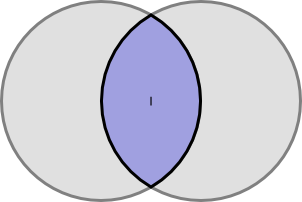
\includegraphics[height=3.03cm]{Figures/1Chapter/intersection}
\end{psfrags}
\caption{The intersection of sets $S$ and $T$ only contains elements that are both in $S$ and $T$.}
\end{center}
\end{figure}

When $S$ and $T$ have no elements in common, we write $S \cap T = \emptyset$.
We also express this fact by saying that $S$ and $T$ are \emph{disjoint}.\index{Disjoint sets}
More generally, a collection of sets is said to be disjoint if no two sets have a common element.
A collection of sets is said to form a \emph{partition} of $S$ if the sets in the collection are disjoint and their union is $S$.\index{Partition}

\begin{figure}[htb]
\begin{center}
\includegraphics[height=3.03cm]{Figures/1Chapter/setpartition}
\caption{A partition of $S$ is a collection of sets that are disjoint and whose union is $S$.}
\end{center}
\end{figure}

The \emph{difference} of two sets, denoted by $S - T$, is defined as the set consisting of those elements of $S$ that are not in $T$, $S - T = \{ x | x \in S \text{ and } x \notin T \}$.
This set is sometimes called the complement of $T$ relative to $S$, or the complement of $T$ in $S$.

\begin{figure}[htb]
\begin{center}
\begin{psfrags}
\psfrag{D}[c]{$S - T$}
\includegraphics[height=3.03cm]{Figures/1Chapter/difference}
\end{psfrags}
\caption{The complement of $T$ relative to $S$ contains all the elements of $S$ that are not in $T$.}
\end{center}
\end{figure}

So far, we have looked at the definition of the union and the intersection of two sets.
We can also form the union or the intersection of arbitrarily many sets.
This is defined in a straightforward way,
\begin{align*}
\bigcup_{\alpha \in \IndexSet} S_{\alpha}
&= \{ x | x \in S_{\alpha} \text{ for some } \alpha \in \IndexSet \} \\
\bigcap_{\alpha \in \IndexSet} S_{\alpha}
&= \{ x | x \in S_{\alpha} \text{ for all } \alpha \in \IndexSet \} .
\end{align*}
The index set $\IndexSet$ can be finite or infinite.


\section{Additional Rules and Properties}

Given a collection of sets, it is possible to form new ones by applying elementary set operations to them.
As in algebra, one uses parentheses to indicate precedence.
For instance, $R \cup (S \cap T)$ denotes the union of two sets $R$ and $S \cap T$, whereas $(R \cup S) \cap T$ represents the intersection of two sets $R \cup S$ and $T$.
The sets thus formed are quite different.

\begin{figure}[htb]
\begin{center}
\begin{psfrags}
\psfrag{P1}[c]{$R \cup (S \cap T)$}
\psfrag{P2}[c]{$(R \cup S) \cap T$}
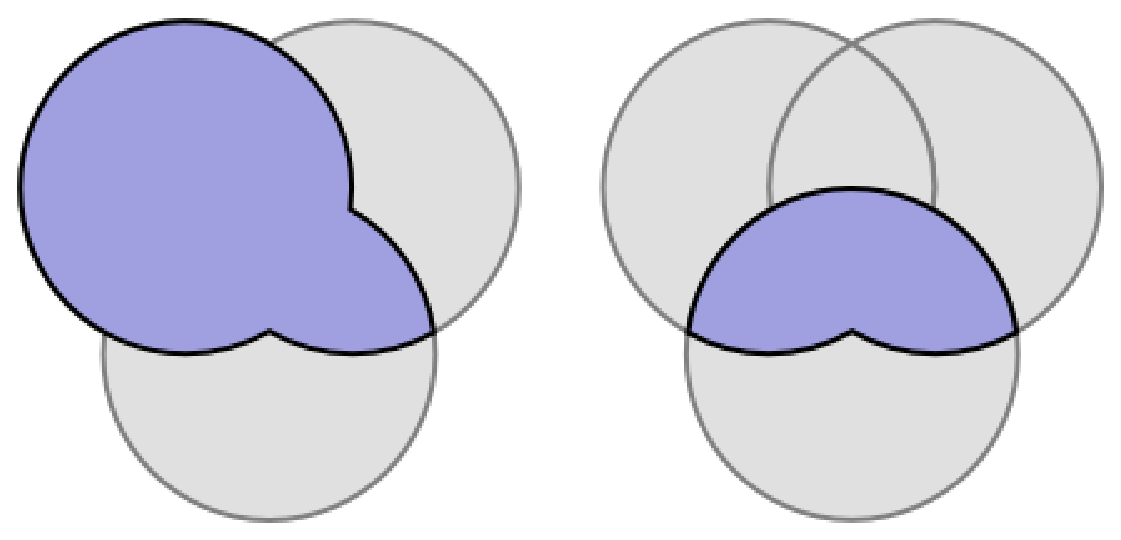
\includegraphics[height=4.55cm]{Figures/1Chapter/triple}
\end{psfrags}
\caption{The order of set operations is important; parentheses should be employed to specify precedence.}
\end{center}
\end{figure}

Sometimes different combinations of operations lead to a same set.
For instance, we have the following distributive laws
\begin{align*}
R \cap (S \cup T) &= (R \cap S) \cup (R \cap T) \\
R \cup (S \cap T) &= (R \cup S) \cap (R \cup T).
\end{align*}
Two particularly useful equivalent combinations of operations are given by \emph{De~Morgan's laws}, which state that\index{De Morgan's laws}
\begin{align*}
R - (S \cup T) &= (R - S) \cap (R - T) \\
R - (S \cap T) &= (R - S) \cup (R - T).
\end{align*}
These two laws can be generalized to
\begin{align*}
\left( \bigcup_{\alpha \in \IndexSet} S_{\alpha} \right)^{\Complement}
&= \bigcap_{\alpha \in \IndexSet} S_{\alpha}^{\Complement} \\
\left( \bigcap_{\alpha \in \IndexSet} S_{\alpha} \right)^{\Complement}
&= \bigcup_{\alpha \in \IndexSet} S_{\alpha}^{\Complement}
\end{align*}
when multiple sets are involved.
To establish the first equality, suppose that $x$ belongs to $\left( \bigcup_{\alpha \in \IndexSet} S_{\alpha} \right)^{\Complement}$.
Then $x$ is not contained in $\bigcup_{\alpha \in \IndexSet} S_{\alpha}$.
That is, $x$ is not an element of $S_{\alpha}$ for any $\alpha \in \IndexSet$.
This implies that $x$ belongs to $S_{\alpha}^{\Complement}$ for all $\alpha \in \IndexSet$, and therefore $x \in \bigcap_{\alpha \in \IndexSet} S_{\alpha}^{\Complement}$.
We have shown that $\left( \bigcup_{\alpha \in \IndexSet} S_{\alpha} \right)^{\Complement} \subset \bigcap_{\alpha \in \IndexSet} S_{\alpha}^{\Complement}$.
The converse inclusion is obtained by reversing the above argument.
The second law can be obtained in a similar fashion.


\section{Cartesian Products}

There is yet another way to create new sets form existing ones.
It involves the notion of an \emph{ordered pair} of objects.\index{Ordered pair}
Given sets $S$ and $T$, the \emph{cartesian product} $S \times T$ is the set of all ordered pairs $(x, y)$ for which $x$ is an element of $S$ and $y$ is an element of $T$, $S \times T = \{ (x, y) | x \in S \text{ and } y \in T \}$.\index{Cartesian product}

\begin{figure}[htb]
\begin{center}
\begin{psfrags}
\psfrag{1}[c]{$1$}
\psfrag{2}[c]{$2$}
\psfrag{3}[c]{$3$}
\psfrag{a}[c]{$a$}
\psfrag{b}[c]{$b$}
\includegraphics[height=3.06cm]{Figures/1Chapter/cartesianproduct}
\end{psfrags}
\caption{Cartesian products can be used to create new sets.
In this example, the sets $\{ 1, 2, 3 \}$ and $\{ a, b \}$ are employed to create a cartesian product with six elements.}
\end{center}
\end{figure}


\section{Set Theory and Probability}

Set theory provides a rigorous foundation for modern probability and its axiomatic basis.
It is employed to describe the laws of probability, give meaning to their implications and answer practical questions.
Being familiar with basic definitions and set operations is key in understanding the subtleties of probability; it helps overcome its many challenges.
A working knowledge of set theory becomes critical when modeling measured quantities and evolving processes that appear random, an invaluable skill for engineers.

 % No psfrags
\chapter{Intuitive Probability and Combinatorics}

The simplest probabilistic scenario is perhaps one where the set of possible outcomes is finite and these outcomes are all equally likely.
A subset of the set of possible outcomes is called an \emph{event}.
Computing the probability of an event amounts to counting the number of elements comprising this event and then dividing the sum by the total number of admissible outcomes.

\begin{example}
The rolling of a fair die is an experiment with a finite number of equally likely outcomes, namely the different faces labeled one through six.
The probability of observing a specific face is equal to
\begin{equation*}
\frac{1}{\text{Number of faces}} = \frac{1}{6} .
\end{equation*}
Similarly, the probability of an arbitrary event can be computed by counting the number of distinct outcomes included in the event.
For instance, the probability of rolling a prime number is
\begin{equation*}
\Pr ( \{ 2, 3, 5 \} )
= \frac{\text{Number of outcomes in event}}{\text{Total number of outcomes}}
= \frac{3}{6} .
\end{equation*}
\end{example}

While counting outcomes may appear intuitively straightforward, it is in many circumstances a daunting task.
Calculating the number of ways that certain patterns can be formed is part of the field of \emph{combinatorics}. \index{Combinatorics}
In this chapter, we introduce useful counting techniques that can be applied to situations pertinent to probability.


\section{The Counting Principle}

The counting principle is a guiding rule for computing the number of elements in a Cartesian product.
Suppose that $S$ and $T$ are finite sets with $m$ and $n$ elements, respectively.
The Cartesian product of $S$ and $T$ is given by
\begin{equation*}
S \times T = \{ (x, y) | x \in S \text{ and } y \in T \} .
\end{equation*}
The number of elements in the Cartesian product $S \times T$ is equal to $m n$.
This is illustrated in Figure~\ref{figure:CountingPrinciple}.

\begin{figure}[htb!]
\begin{center}
% FIGURE GROUP = BALLS
\begin{footnotesize}
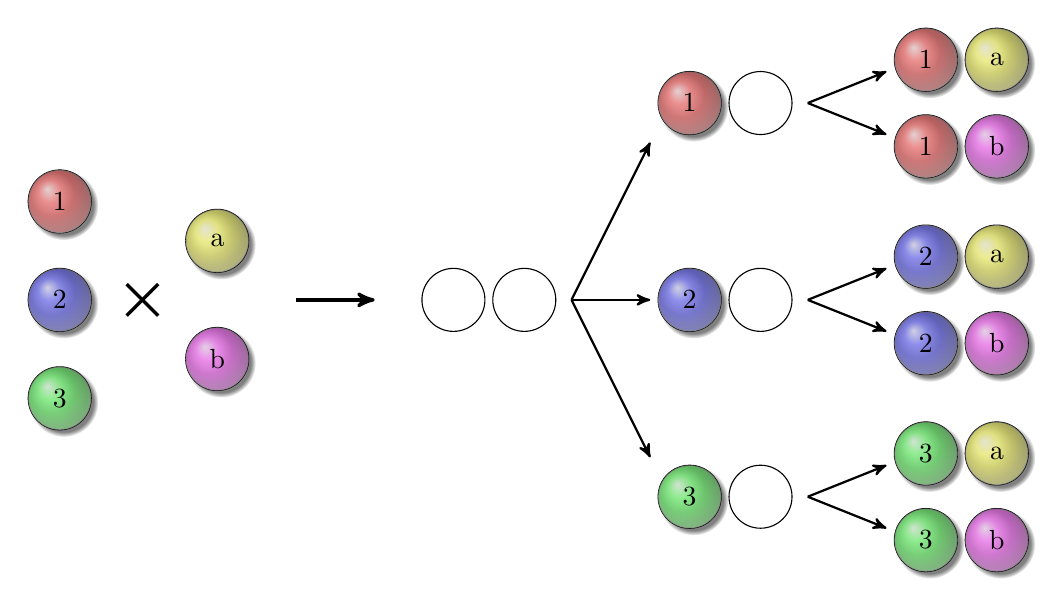
\begin{tikzpicture}
\shade[draw=black, ball color=red, circular drop shadow] (0,1.25) circle (4mm);
\shade[fill=white, fill opacity=0.3] (0,1.25) circle (4mm) node[fill opacity=1]{1};

\shade[draw=black, ball color=blue, circular drop shadow] (0,0) circle (4mm);
\shade[fill=white, fill opacity=0.3] (0,0) circle (4mm) node[fill opacity=1]{2};

\shade[draw=black, ball color=green, circular drop shadow] (0,-1.25) circle (4mm);
\shade[fill=white, fill opacity=0.3] (0,-1.25) circle (4mm) node[fill opacity=1]{3};

\draw[very thick] (0.85,-0.2) -- (1.25,0.2);
\draw[very thick] (0.85,0.2) -- (1.25,-0.2);

\shade[draw=black, ball color=yellow, circular drop shadow] (2,0.75) circle (4mm);
\shade[fill=white, fill opacity=0.3] (2,0.75) circle (4mm) node[fill opacity=1]{$\mathrm{a}$};

\shade[draw=black, ball color=magenta, circular drop shadow] (2,-0.75) circle (4mm);
\shade[fill=white, fill opacity=0.3] (2,-0.75) circle (4mm) node[fill opacity=1]{$\mathrm{b}$};

\draw[very thick, ->, >=stealth'] (3,0) -- (4,0);

\draw[draw=black] (5,0) circle (4mm);
\draw[draw=black] (5.9,0) circle (4mm);

\draw[thick, ->, >=stealth'] (6.5,0) -- (7.5,2);
\draw[thick, ->, >=stealth'] (6.5,0) -- (7.5,0);
\draw[thick, ->, >=stealth'] (6.5,0) -- (7.5,-2);

\shade[draw=black, ball color=red, circular drop shadow] (8,2.5) circle (4mm);
\shade[fill=white, fill opacity=0.3] (8,2.5) circle (4mm) node[fill opacity=1]{1};
\draw[draw=black] (8.9,2.5) circle (4mm);

\shade[draw=black, ball color=blue, circular drop shadow] (8,0) circle (4mm);
\shade[fill=white, fill opacity=0.3] (8,0) circle (4mm) node[fill opacity=1]{2};
\draw[draw=black] (8.9,0) circle (4mm);

\shade[draw=black, ball color=green, circular drop shadow] (8,-2.5) circle (4mm);
\shade[fill=white, fill opacity=0.3] (8,-2.5) circle (4mm) node[fill opacity=1]{3};
\draw[draw=black] (8.9,-2.5) circle (4mm);

\draw[thick, ->, >=stealth'] (9.5,2.5) -- (10.5,2.9);
\draw[thick, ->, >=stealth'] (9.5,2.5) -- (10.5,2.1);

\draw[thick, ->, >=stealth'] (9.5,0) -- (10.5,0.4);
\draw[thick, ->, >=stealth'] (9.5,0) -- (10.5,-0.4);

\draw[thick, ->, >=stealth'] (9.5,-2.5) -- (10.5,-2.1);
\draw[thick, ->, >=stealth'] (9.5,-2.5) -- (10.5,-2.9);

\shade[draw=black, ball color=red, circular drop shadow] (11,3.05) circle (4mm);
\shade[fill=white, fill opacity=0.3] (11,3.05) circle (4mm) node[fill opacity=1]{1};
\shade[draw=black, ball color=yellow, circular drop shadow] (11.9,3.05) circle (4mm);
\shade[fill=white, fill opacity=0.3] (11.9,3.05) circle (4mm) node[fill opacity=1]{$\mathrm{a}$};

\shade[draw=black, ball color=red, circular drop shadow] (11,1.95) circle (4mm);
\shade[fill=white, fill opacity=0.3] (11,1.95) circle (4mm) node[fill opacity=1]{1};
\shade[draw=black, ball color=magenta, circular drop shadow] (11.9,1.95) circle (4mm);
\shade[fill=white, fill opacity=0.3] (11.9,1.95) circle (4mm) node[fill opacity=1]{$\mathrm{b}$};

\shade[draw=black, ball color=blue, circular drop shadow] (11,0.55) circle (4mm);
\shade[fill=white, fill opacity=0.3] (11,0.55) circle (4mm) node[fill opacity=1]{2};
\shade[draw=black, ball color=yellow, circular drop shadow] (11.9,0.55) circle (4mm);
\shade[fill=white, fill opacity=0.3] (11.9,0.55) circle (4mm) node[fill opacity=1]{$\mathrm{a}$};

\shade[draw=black, ball color=blue, circular drop shadow] (11,-0.55) circle (4mm);
\shade[fill=white, fill opacity=0.3] (11,-0.55) circle (4mm) node[fill opacity=1]{2};
\shade[draw=black, ball color=magenta, circular drop shadow] (11.9,-0.55) circle (4mm);
\shade[fill=white, fill opacity=0.3] (11.9,-0.55) circle (4mm) node[fill opacity=1]{$\mathrm{b}$};

\shade[draw=black, ball color=green, circular drop shadow] (11,-1.95) circle (4mm);
\shade[fill=white, fill opacity=0.3] (11,-1.95) circle (4mm) node[fill opacity=1]{3};
\shade[draw=black, ball color=yellow, circular drop shadow] (11.9,-1.95) circle (4mm);
\shade[fill=white, fill opacity=0.3] (11.9,-1.95) circle (4mm) node[fill opacity=1]{$\mathrm{a}$};

\shade[draw=black, ball color=green, circular drop shadow] (11,-3.05) circle (4mm);
\shade[fill=white, fill opacity=0.3] (11,-3.05) circle (4mm) node[fill opacity=1]{3};
\shade[draw=black, ball color=magenta, circular drop shadow] (11.9,-3.05) circle (4mm);
\shade[fill=white, fill opacity=0.3] (11.9,-3.05) circle (4mm) node[fill opacity=1]{$\mathrm{b}$};
\end{tikzpicture}
\end{footnotesize}
\caption{This figure provides a graphical interpretation of the Cartesian product of $S = \{ 1, 2, 3 \}$ and $T = \{ \mathrm{a}, \mathrm{b} \}$.
In general, if $S$ has $m$ elements and $T$ contains $n$ elements, then the Cartesian product $S \times T$ consists of $m n$ elements.}
\label{figure:CountingPrinciple}
\end{center}
\end{figure}

\begin{example}
Consider an experiment consisting of flipping a coin and rolling a die.
There are two possibilities for the coin, heads or tails, and the die has six faces.
The number of possible outcomes for this experiment is $2 \times 6 = 12$.
That is, there are twelve different ways to flip a coin and roll a die.
\end{example}

Using the equally likely outcome model, the above example implies that the probability of each outcome is $\frac{1}{2} \cdot \frac{1}{6} = \frac{1}{12}$.
As we will eventually see, this is an instance of the \emph{product rule} for \emph{independent} experiments, which says the probability that two events both occur is given by the product of their individual probabilities if and only if they are independent.
For now, we will interpet the word independent intuitively and take it to mean that the two experiments have no relation to each other.

\begin{example}
Consider two experiments and let $S_1$ be the set of outcomes for the first and $S_2$ be the set of outcomes for the second.
Let $E_1 \subseteq S_1$ and $E_2 \subseteq S_2$ be events of interest for the two experiments.
One can think of the two experiments together as a single experiment with outcomes $S = S_1 \times S_2$.
In this model, the set of joint outcomes where $E_1$ and $E_2$ both occur is given by the joint event $E = E_1 \times E_2$.
The equally likely outcome model for this joint experiment asserts that the probability that both events occur is given by
\[ \frac{|E|}{|S|} = \frac{|E_1 \times E_2|}{|S_1 \times S_2|} = \frac{|E_1|\,|E_2|}{|S_1|\,|S_2|} = \frac{|E_1|}{|S_1|}\,\frac{|E_2|}{|S_2|}. \]
This implies that the product rule is correct when equally-likely experiments are combined this way.
Conversely, events are called independent only if the product rule works.
Therefore, combining multiple experiments in this way is the same as assuming they are independent.
\end{example}

The counting principle can be broadened to calculating the number of elements in the Cartesian product of multiple sets.
Consider the finite sets $S_1, S_2, \ldots, S_r$ and their Cartesian product
\begin{equation*}
S_1 \times S_2 \times \cdots \times S_r
= \left\{ (s_1, s_2, \ldots, s_r) | s_i \in S_i \right\} .
\end{equation*}
If we denote the cardinality of $S_i$ by $n_i = | S_i |$, then the number of distinct ordered $r$-tuples of the form $(s_1, s_2, \ldots, s_r)$ is $n = n_1 n_2 \cdots n_r$.

\begin{example}[Sampling with Replacement and Ordering]
An urn contains $n$ balls numbered one through $n$.
A ball is drawn from the urn and its number is recorded on an ordered list.
The ball is then replaced in the urn.
This procedure is repeated $k$ times.
We wish to compute the number of possible sequences that can result from this experiment.
There are $k$ drawings and $n$ possibilities per drawing.
Using the counting principle, we gather that the number of distinct sequences is $n^k$.

\begin{figure}[htb!]
\begin{center}
% FIGURE GROUP = BALLS
\begin{footnotesize}
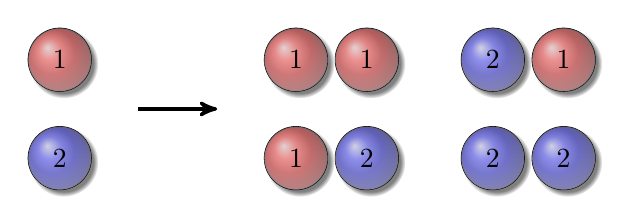
\begin{tikzpicture}
\shade[draw=black, ball color=red, circular drop shadow] (0,0.625) circle (4mm);
\shade[fill=white, fill opacity=0.3] (0,0.625) circle (4mm) node[fill opacity=1]{1};

\shade[draw=black, ball color=blue, circular drop shadow] (0,-0.625) circle (4mm);
\shade[fill=white, fill opacity=0.3] (0,-0.625) circle (4mm) node[fill opacity=1]{2};

\draw[very thick, ->, >=stealth'] (1,0) -- (2,0);

\shade[draw=black, ball color=red, circular drop shadow] (3,0.625) circle (4mm);
\shade[fill=white, fill opacity=0.3] (3,0.625) circle (4mm) node[fill opacity=1]{1};
\shade[draw=black, ball color=red, circular drop shadow] (3.9,0.625) circle (4mm);
\shade[fill=white, fill opacity=0.3] (3.9,0.625) circle (4mm) node[fill opacity=1]{1};

\shade[draw=black, ball color=red, circular drop shadow] (3,-0.625) circle (4mm);
\shade[fill=white, fill opacity=0.3] (3,-0.625) circle (4mm) node[fill opacity=1]{1};
\shade[draw=black, ball color=blue, circular drop shadow] (3.9,-0.625) circle (4mm);
\shade[fill=white, fill opacity=0.3] (3.9,-0.625) circle (4mm) node[fill opacity=1]{2};

\shade[draw=black, ball color=blue, circular drop shadow] (5.5,0.625) circle (4mm);
\shade[fill=white, fill opacity=0.3] (5.5,0.625) circle (4mm) node[fill opacity=1]{2};
\shade[draw=black, ball color=red, circular drop shadow] (6.4,0.625) circle (4mm);
\shade[fill=white, fill opacity=0.3] (6.4,0.625) circle (4mm) node[fill opacity=1]{1};

\shade[draw=black, ball color=blue, circular drop shadow] (5.5,-0.625) circle (4mm);
\shade[fill=white, fill opacity=0.3] (5.5,-0.625) circle (4mm) node[fill opacity=1]{2};
\shade[draw=black, ball color=blue, circular drop shadow] (6.4,-0.625) circle (4mm);
\shade[fill=white, fill opacity=0.3] (6.4,-0.625) circle (4mm) node[fill opacity=1]{2};
\end{tikzpicture}
\end{footnotesize}
\caption{The Cartesian product $\{ 1, 2 \}^2$ has four distinct ordered pairs.}
\label{figure:Sequences}
\end{center}
\end{figure}
\end{example}

\begin{example}
The \emph{power set} of $S$, denoted by $2^S$, is the collection of all subsets of $S$. \index{Power set}
In set theory, $2^S$ represents the set of all functions from $S$ to $\{ 0, 1\}$.
By identifying a function in $2^S$ with the corresponding preimage of one, we obtain a bijection between $2^S$ and the subsets of $S$.
In particular, each function in $2^S$ is the characteristic function of a subset of $S$.

Suppose that $S$ is finite with $n = |S|$ elements.
For every element of $S$, a characteristic function in $2^S$ is either zero or one.
There are therefore $2^n$ distinct characteristic functions from $S$ to $\{ 0, 1\}$.
Hence, the number of distinct subsets of $S$ is given by $2^n$.

\begin{figure}[htb!]
\begin{center}
% FIGURE GROUP = BALLS
\begin{footnotesize}
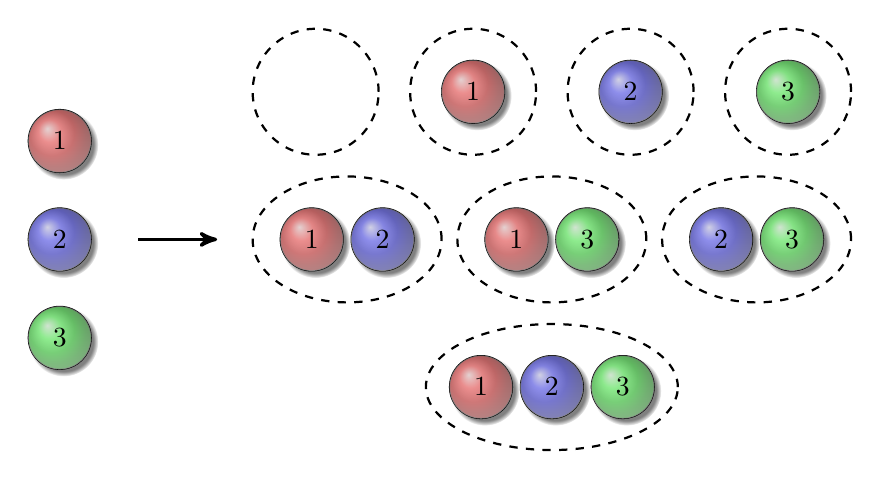
\begin{tikzpicture}
\shade[draw=black, ball color=red, circular drop shadow] (0,1.25) circle (4mm);
\shade[fill=white, fill opacity=0.3] (0,1.25) circle (4mm) node[fill opacity=1]{1};

\shade[draw=black, ball color=blue, circular drop shadow] (0,0) circle (4mm);
\shade[fill=white, fill opacity=0.3] (0,0) circle (4mm) node[fill opacity=1]{2};

\shade[draw=black, ball color=green, circular drop shadow] (0,-1.25) circle (4mm);
\shade[fill=white, fill opacity=0.3] (0,-1.25) circle (4mm) node[fill opacity=1]{3};

\draw[very thick, ->, >=stealth'] (1,0) -- (2,0);

\draw[color=black, thick, dashed] (3.25,1.875) circle (8mm);

\draw[color=black, thick, dashed] (5.25,1.875) circle (8mm);
\shade[draw=black, ball color=red, circular drop shadow] (5.25,1.875) circle (4mm);
\shade[fill=white, fill opacity=0.3] (5.25,1.875) circle (4mm) node[fill opacity=1]{1};

\draw[color=black, thick, dashed] (7.25,1.875) circle (8mm);
\shade[draw=black, ball color=blue, circular drop shadow] (7.25,1.875) circle (4mm);
\shade[fill=white, fill opacity=0.3] (7.25,1.875) circle (4mm) node[fill opacity=1]{2};

\draw[color=black, thick, dashed] (9.25,1.875) circle (8mm);
\shade[draw=black, ball color=green, circular drop shadow] (9.25,1.875) circle (4mm);
\shade[fill=white, fill opacity=0.3] (9.25,1.875) circle (4mm) node[fill opacity=1]{3};

\draw[color=black, thick, dashed] (3.65,0) ellipse (12mm and 8mm);
\shade[draw=black, ball color=red, circular drop shadow] (3.2,0) circle (4mm);
\shade[fill=white, fill opacity=0.3] (3.2,0) circle (4mm) node[fill opacity=1]{1};
\shade[draw=black, ball color=blue, circular drop shadow] (4.1,0) circle (4mm);
\shade[fill=white, fill opacity=0.3] (4.1,0) circle (4mm) node[fill opacity=1]{2};

\draw[color=black, thick, dashed] (6.25,0) ellipse (12mm and 8mm);
\shade[draw=black, ball color=red, circular drop shadow] (5.8,0) circle (4mm);
\shade[fill=white, fill opacity=0.3] (5.8,0) circle (4mm) node[fill opacity=1]{1};
\shade[draw=black, ball color=green, circular drop shadow] (6.7,0) circle (4mm);
\shade[fill=white, fill opacity=0.3] (6.7,0) circle (4mm) node[fill opacity=1]{3};

\draw[color=black, thick, dashed] (8.85,0) ellipse (12mm and 8mm);
\shade[draw=black, ball color=blue, circular drop shadow] (8.4,0) circle (4mm);
\shade[fill=white, fill opacity=0.3] (8.4,0) circle (4mm) node[fill opacity=1]{2};
\shade[draw=black, ball color=green, circular drop shadow] (9.3,0) circle (4mm);
\shade[fill=white, fill opacity=0.3] (9.3,0) circle (4mm) node[fill opacity=1]{3};

\draw[color=black, thick, dashed] (6.25,-1.875) ellipse (16mm and 8mm);
\shade[draw=black, ball color=red, circular drop shadow] (5.35,-1.875) circle (4mm);
\shade[fill=white, fill opacity=0.3] (5.35,-1.875) circle (4mm) node[fill opacity=1]{1};
\shade[draw=black, ball color=blue, circular drop shadow] (6.25,-1.875) circle (4mm);
\shade[fill=white, fill opacity=0.3] (6.25,-1.875) circle (4mm) node[fill opacity=1]{2};
\shade[draw=black, ball color=green, circular drop shadow] (7.15,-1.875) circle (4mm);
\shade[fill=white, fill opacity=0.3] (7.15,-1.875) circle (4mm) node[fill opacity=1]{3};
\end{tikzpicture}
\end{footnotesize}
\caption{The power set of $\{ 1, 2, 3 \}$ contains eight subsets.
These elements are displayed above.}
\label{figure:PowerSet}
\end{center}
\end{figure}
\end{example}


\section{Permutations}

Again, consider the integer set $S = \{ 1, 2, \ldots, n \}$.
A \emph{permutation} of $S$ is an ordered arrangement of its elements, i.e., a list without repetitions. \index{Permutation}
The number of permutations of $S$ can be computed using the following argument.
Clearly, there are $n$ distinct possibilities for the first item in the list.
The number of possibilities for the second item is $n-1$, namely all the integers in $S$ except the element we selected initially.
Similarly, the number of distinct possibilities for the $m$th item is $n - m + 1$.
This pattern continues until all the elements in $S$ are recorded.
Summarizing, we find that the total number of permutations of $S$ is $n$ \emph{factorial}, $n! = n (n-1) \cdots 1$. \index{Factorial}

\begin{example}
We wish to compute the number of permutations of $S = \{ 1, 2, 3 \}$.
Since the set $S$ possesses three elements, it has $3! = 6$ different permutations.
They can be written as $123, 132, 213, 231, 312, 321$.
\end{example}

\begin{figure}[htb!]
\begin{center}
% FIGURE GROUP = BALLS
\begin{footnotesize}
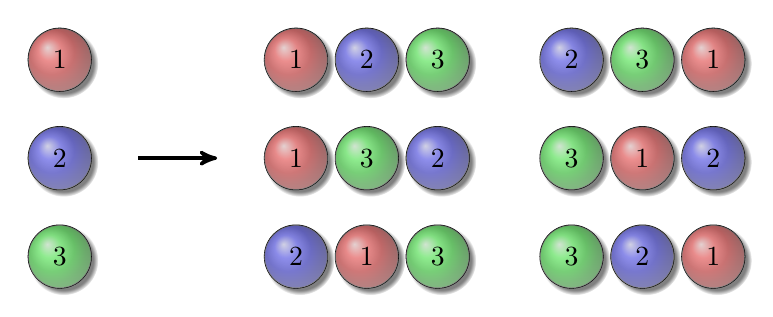
\begin{tikzpicture}
\shade[draw=black, ball color=red, circular drop shadow] (0,1.25) circle (4mm);
\shade[fill=white, fill opacity=0.3] (0,1.25) circle (4mm) node[fill opacity=1]{1};

\shade[draw=black, ball color=blue, circular drop shadow] (0,0) circle (4mm);
\shade[fill=white, fill opacity=0.3] (0,0) circle (4mm) node[fill opacity=1]{2};

\shade[draw=black, ball color=green, circular drop shadow] (0,-1.25) circle (4mm);
\shade[fill=white, fill opacity=0.3] (0,-1.25) circle (4mm) node[fill opacity=1]{3};

\draw[very thick, ->, >=stealth'] (1,0) -- (2,0);

\shade[draw=black, ball color=red, circular drop shadow] (3,1.25) circle (4mm);
\shade[fill=white, fill opacity=0.3] (3,1.25) circle (4mm) node[fill opacity=1]{1};
\shade[draw=black, ball color=blue, circular drop shadow] (3.9,1.25) circle (4mm);
\shade[fill=white, fill opacity=0.3] (3.9,1.25) circle (4mm) node[fill opacity=1]{2};
\shade[draw=black, ball color=green, circular drop shadow] (4.8,1.25) circle (4mm);
\shade[fill=white, fill opacity=0.3] (4.8,1.25) circle (4mm) node[fill opacity=1]{3};

\shade[draw=black, ball color=red, circular drop shadow] (3,0) circle (4mm);
\shade[fill=white, fill opacity=0.3] (3,0) circle (4mm) node[fill opacity=1]{1};
\shade[draw=black, ball color=green, circular drop shadow] (3.9,0) circle (4mm);
\shade[fill=white, fill opacity=0.3] (3.9,0) circle (4mm) node[fill opacity=1]{3};
\shade[draw=black, ball color=blue, circular drop shadow] (4.8,0) circle (4mm);
\shade[fill=white, fill opacity=0.3] (4.8,0) circle (4mm) node[fill opacity=1]{2};

\shade[draw=black, ball color=blue, circular drop shadow] (3,-1.25) circle (4mm);
\shade[fill=white, fill opacity=0.3] (3,-1.25) circle (4mm) node[fill opacity=1]{2};
\shade[draw=black, ball color=red, circular drop shadow] (3.9,-1.25) circle (4mm);
\shade[fill=white, fill opacity=0.3] (3.9,-1.25) circle (4mm) node[fill opacity=1]{1};
\shade[draw=black, ball color=green, circular drop shadow] (4.8,-1.25) circle (4mm);
\shade[fill=white, fill opacity=0.3] (4.8,-1.25) circle (4mm) node[fill opacity=1]{3};

\shade[draw=black, ball color=blue, circular drop shadow] (6.5,1.25) circle (4mm);
\shade[fill=white, fill opacity=0.3] (6.5,1.25) circle (4mm) node[fill opacity=1]{2};
\shade[draw=black, ball color=green, circular drop shadow] (7.4,1.25) circle (4mm);
\shade[fill=white, fill opacity=0.3] (7.4,1.25) circle (4mm) node[fill opacity=1]{3};
\shade[draw=black, ball color=red, circular drop shadow] (8.3,1.25) circle (4mm);
\shade[fill=white, fill opacity=0.3] (8.3,1.25) circle (4mm) node[fill opacity=1]{1};

\shade[draw=black, ball color=green, circular drop shadow] (6.5,0) circle (4mm);
\shade[fill=white, fill opacity=0.3] (6.5,0) circle (4mm) node[fill opacity=1]{3};
\shade[draw=black, ball color=red, circular drop shadow] (7.4,0) circle (4mm);
\shade[fill=white, fill opacity=0.3] (7.4,0) circle (4mm) node[fill opacity=1]{1};
\shade[draw=black, ball color=blue, circular drop shadow] (8.3,0) circle (4mm);
\shade[fill=white, fill opacity=0.3] (8.3,0) circle (4mm) node[fill opacity=1]{2};

\shade[draw=black, ball color=green, circular drop shadow] (6.5,-1.25) circle (4mm);
\shade[fill=white, fill opacity=0.3] (6.5,-1.25) circle (4mm) node[fill opacity=1]{3};
\shade[draw=black, ball color=blue, circular drop shadow] (7.4,-1.25) circle (4mm);
\shade[fill=white, fill opacity=0.3] (7.4,-1.25) circle (4mm) node[fill opacity=1]{2};
\shade[draw=black, ball color=red, circular drop shadow] (8.3,-1.25) circle (4mm);
\shade[fill=white, fill opacity=0.3] (8.3,-1.25) circle (4mm) node[fill opacity=1]{1};
\end{tikzpicture}
\end{footnotesize}
\caption{Ordering the numbers one, two and three leads to six possible permutations.}
\label{figure:Permutation}
\end{center}
\end{figure}


\subsection{Stirling's Formula*}

The number $n!$ grows very rapidly as a function of $n$.
A good approximation for $n!$ when $n$ is large is given by \emph{Stirling's formula}, \index{Stirling's formula}
\begin{equation*}
n! \sim n^n e^{-n} \sqrt{ 2 \pi n} .
\end{equation*}
The notation $a_n \sim b_n$ signifies that the ratio $a_n / b_n \rightarrow 1$ as $n \rightarrow \infty$.


\subsection{k-Permutations}

Suppose that we rank only $k$ elements out of the set $S = \{ 1, 2, \ldots, n \}$, where $k \leq n$.
We wish to count the number of distinct $k$-permutations of $S$.
Following our previous argument, we can choose one of $n$ elements to be the first item listed, one of the remaining $(n-1)$ elements for the second item, and so on.
The procedure terminates when $k$ items have been recorded.
The number of possible sequences is therefore given by
\begin{equation*}
\frac{n!}{(n-k)!} = n (n-1) \cdots (n-k+1) .
\end{equation*}

\begin{example}
A recently formed music group can play four original songs.
They are asked to perform two songs at South by Southwest.
We wish to compute the number of song arrangements the group can offer in concert.
Abstractly, this is equivalent to computing the number of $2$-permutations of four songs.
Thus, the number of distinct arrangements is ${4!}/{2!} = 12$.
\end{example}

\begin{figure}[htb!]
\begin{center}
% FIGURE GROUP = BALLS
\begin{footnotesize}
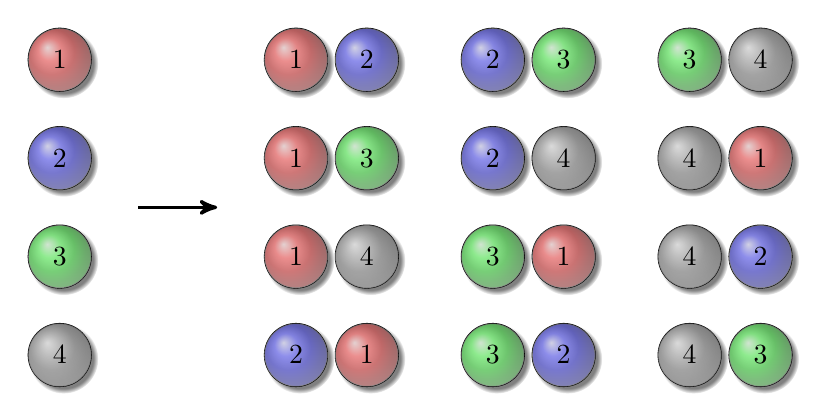
\begin{tikzpicture}
\shade[draw=black, ball color=red, circular drop shadow] (0,1.875) circle (4mm);
\shade[fill=white, fill opacity=0.3] (0,1.875) circle (4mm) node[fill opacity=1]{1};

\shade[draw=black, ball color=blue, circular drop shadow] (0,0.625) circle (4mm);
\shade[fill=white, fill opacity=0.3] (0,0.625) circle (4mm) node[fill opacity=1]{2};

\shade[draw=black, ball color=green, circular drop shadow] (0,-0.625) circle (4mm);
\shade[fill=white, fill opacity=0.3] (0,-0.625) circle (4mm) node[fill opacity=1]{3};

\shade[draw=black, ball color=gray, circular drop shadow] (0,-1.875) circle (4mm);
\shade[fill=white, fill opacity=0.3] (0,-1.875) circle (4mm) node[fill opacity=1]{4};

\draw[very thick, ->, >=stealth'] (1,0) -- (2,0);

\shade[draw=black, ball color=red, circular drop shadow] (3,1.875) circle (4mm);
\shade[fill=white, fill opacity=0.3] (3,1.875) circle (4mm) node[fill opacity=1]{1};
\shade[draw=black, ball color=blue, circular drop shadow] (3.9,1.875) circle (4mm);
\shade[fill=white, fill opacity=0.3] (3.9,1.875) circle (4mm) node[fill opacity=1]{2};

\shade[draw=black, ball color=red, circular drop shadow] (3,0.625) circle (4mm);
\shade[fill=white, fill opacity=0.3] (3,0.625) circle (4mm) node[fill opacity=1]{1};
\shade[draw=black, ball color=green, circular drop shadow] (3.9,0.625) circle (4mm);
\shade[fill=white, fill opacity=0.3] (3.9,0.625) circle (4mm) node[fill opacity=1]{3};

\shade[draw=black, ball color=red, circular drop shadow] (3,-0.625) circle (4mm);
\shade[fill=white, fill opacity=0.3] (3,-0.625) circle (4mm) node[fill opacity=1]{1};
\shade[draw=black, ball color=gray, circular drop shadow] (3.9,-0.625) circle (4mm);
\shade[fill=white, fill opacity=0.3] (3.9,-0.625) circle (4mm) node[fill opacity=1]{4};

\shade[draw=black, ball color=blue, circular drop shadow] (3,-1.875) circle (4mm);
\shade[fill=white, fill opacity=0.3] (3,-1.875) circle (4mm) node[fill opacity=1]{2};
\shade[draw=black, ball color=red, circular drop shadow] (3.9,-1.875) circle (4mm);
\shade[fill=white, fill opacity=0.3] (3.9,-1.875) circle (4mm) node[fill opacity=1]{1};

\shade[draw=black, ball color=blue, circular drop shadow] (5.5,1.875) circle (4mm);
\shade[fill=white, fill opacity=0.3] (5.5,1.875) circle (4mm) node[fill opacity=1]{2};
\shade[draw=black, ball color=green, circular drop shadow] (6.4,1.875) circle (4mm);
\shade[fill=white, fill opacity=0.3] (6.4,1.875) circle (4mm) node[fill opacity=1]{3};

\shade[draw=black, ball color=blue, circular drop shadow] (5.5,0.625) circle (4mm);
\shade[fill=white, fill opacity=0.3] (5.5,0.625) circle (4mm) node[fill opacity=1]{2};
\shade[draw=black, ball color=gray, circular drop shadow] (6.4,0.625) circle (4mm);
\shade[fill=white, fill opacity=0.3] (6.4,0.625) circle (4mm) node[fill opacity=1]{4};

\shade[draw=black, ball color=green, circular drop shadow] (5.5,-0.625) circle (4mm);
\shade[fill=white, fill opacity=0.3] (5.5,-0.625) circle (4mm) node[fill opacity=1]{3};
\shade[draw=black, ball color=red, circular drop shadow] (6.4,-0.625) circle (4mm);
\shade[fill=white, fill opacity=0.3] (6.4,-0.625) circle (4mm) node[fill opacity=1]{1};

\shade[draw=black, ball color=green, circular drop shadow] (5.5,-1.875) circle (4mm);
\shade[fill=white, fill opacity=0.3] (5.5,-1.875) circle (4mm) node[fill opacity=1]{3};
\shade[draw=black, ball color=blue, circular drop shadow] (6.4,-1.875) circle (4mm);
\shade[fill=white, fill opacity=0.3] (6.4,-1.875) circle (4mm) node[fill opacity=1]{2};

\shade[draw=black, ball color=green, circular drop shadow] (8,1.875) circle (4mm);
\shade[fill=white, fill opacity=0.3] (8,1.875) circle (4mm) node[fill opacity=1]{3};
\shade[draw=black, ball color=gray, circular drop shadow] (8.9,1.875) circle (4mm);
\shade[fill=white, fill opacity=0.3] (8.9,1.875) circle (4mm) node[fill opacity=1]{4};

\shade[draw=black, ball color=gray, circular drop shadow] (8,0.625) circle (4mm);
\shade[fill=white, fill opacity=0.3] (8,0.625) circle (4mm) node[fill opacity=1]{4};
\shade[draw=black, ball color=red, circular drop shadow] (8.9,0.625) circle (4mm);
\shade[fill=white, fill opacity=0.3] (8.9,0.625) circle (4mm) node[fill opacity=1]{1};

\shade[draw=black, ball color=gray, circular drop shadow] (8,-0.625) circle (4mm);
\shade[fill=white, fill opacity=0.3] (8,-0.625) circle (4mm) node[fill opacity=1]{4};
\shade[draw=black, ball color=blue, circular drop shadow] (8.9,-0.625) circle (4mm);
\shade[fill=white, fill opacity=0.3] (8.9,-0.625) circle (4mm) node[fill opacity=1]{2};

\shade[draw=black, ball color=gray, circular drop shadow] (8,-1.875) circle (4mm);
\shade[fill=white, fill opacity=0.3] (8,-1.875) circle (4mm) node[fill opacity=1]{4};
\shade[draw=black, ball color=green, circular drop shadow] (8.9,-1.875) circle (4mm);
\shade[fill=white, fill opacity=0.3] (8.9,-1.875) circle (4mm) node[fill opacity=1]{3};
\end{tikzpicture}
\end{footnotesize}
\caption{There are twelve 2-permutations of the numbers one through four.}
\label{figure:Kpermutation}
\end{center}
\end{figure}

\begin{example}[Sampling without Replacement, with  Ordering]
An urn contains $n$ balls numbered one through $n$.
A ball is picked from the urn, and its number is recorded on an ordered list.
The ball is not replaced in the urn.
This procedure is repeated until $k$ balls are selected from the urn, where $k \leq n$.
We wish to compute the number of possible sequences that can result from this experiment.
The number of possibilities is equivalent to the number of $k$-permutations of $n$ elements, which is given by $n! / (n-k)!$.
\end{example}


\section{Combinations}

Consider the integer set $S = \{ 1, 2, \ldots, n \}$.
A \emph{combination} is a subset of $S$. \index{Combination}
We emphasize that a combination differs from a permutation in that elements in a combination have no specific ordering.
The $2$-element subsets of $S = \{ 1, 2, 3, 4 \}$ are
\begin{equation*}
\{ 1, 2 \}, \{ 1, 3 \}, \{ 1, 4 \}, \{ 2, 3 \}, \{ 2, 4 \}, \{ 3, 4 \} ,
\end{equation*}
whereas the $2$-permutations of $S$ are more numerous with
\begin{equation*}
\begin{split}
&( 1, 2 ), ( 1, 3 ), ( 1, 4 ), ( 2, 1 ), ( 2, 3 ), ( 2, 4 ), \\
&( 3, 1 ), ( 3, 2 ), ( 3, 4 ), ( 4, 1 ), ( 4, 2 ), ( 4, 3 ) .
\end{split}
\end{equation*}
Consequently, there are fewer $2$-element subsets of $S$ than $2$-permutations of $S$.

\begin{figure}[htb!]
\begin{center}
% FIGURE GROUP = BALLS
\begin{footnotesize}
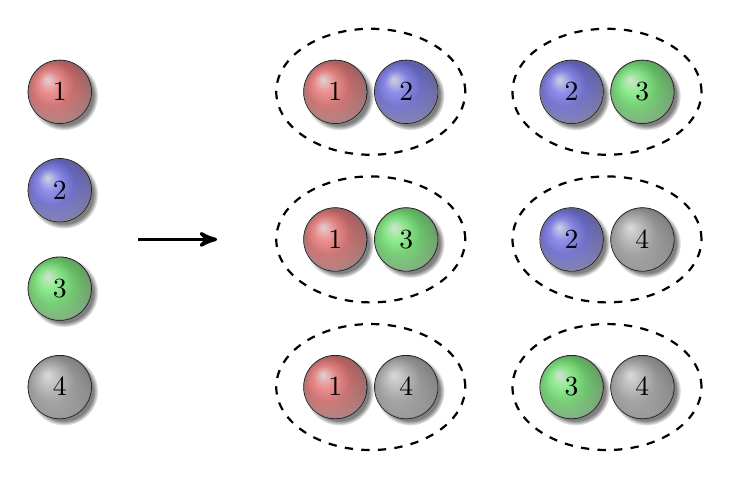
\begin{tikzpicture}
\shade[draw=black, ball color=red, circular drop shadow] (0,1.875) circle (4mm);
\shade[fill=white, fill opacity=0.3] (0,1.875) circle (4mm) node[fill opacity=1]{1};

\shade[draw=black, ball color=blue, circular drop shadow] (0,0.625) circle (4mm);
\shade[fill=white, fill opacity=0.3] (0,0.625) circle (4mm) node[fill opacity=1]{2};

\shade[draw=black, ball color=green, circular drop shadow] (0,-0.625) circle (4mm);
\shade[fill=white, fill opacity=0.3] (0,-0.625) circle (4mm) node[fill opacity=1]{3};

\shade[draw=black, ball color=gray, circular drop shadow] (0,-1.875) circle (4mm);
\shade[fill=white, fill opacity=0.3] (0,-1.875) circle (4mm) node[fill opacity=1]{4};

\draw[very thick, ->, >=stealth'] (1,0) -- (2,0);

\draw[color=black, thick, dashed] (3.95,1.875) ellipse (12mm and 8mm);
\shade[draw=black, ball color=red, circular drop shadow] (3.5,1.875) circle (4mm);
\shade[fill=white, fill opacity=0.3] (3.5,1.875) circle (4mm) node[fill opacity=1]{1};
\shade[draw=black, ball color=blue, circular drop shadow] (4.4,1.875) circle (4mm);
\shade[fill=white, fill opacity=0.3] (4.4,1.875) circle (4mm) node[fill opacity=1]{2};

\draw[color=black, thick, dashed] (3.95,0) ellipse (12mm and 8mm);
\shade[draw=black, ball color=red, circular drop shadow] (3.5,0) circle (4mm);
\shade[fill=white, fill opacity=0.3] (3.5,0) circle (4mm) node[fill opacity=1]{1};
\shade[draw=black, ball color=green, circular drop shadow] (4.4,0) circle (4mm);
\shade[fill=white, fill opacity=0.3] (4.4,0) circle (4mm) node[fill opacity=1]{3};

\draw[color=black, thick, dashed] (3.95,-1.875) ellipse (12mm and 8mm);
\shade[draw=black, ball color=red, circular drop shadow] (3.5,-1.875) circle (4mm);
\shade[fill=white, fill opacity=0.3] (3.5,-1.875) circle (4mm) node[fill opacity=1]{1};
\shade[draw=black, ball color=gray, circular drop shadow] (4.4,-1.875) circle (4mm);
\shade[fill=white, fill opacity=0.3] (4.4,-1.875) circle (4mm) node[fill opacity=1]{4};

\draw[color=black, thick, dashed] (6.95,1.875) ellipse (12mm and 8mm);
\shade[draw=black, ball color=blue, circular drop shadow] (6.5,1.875) circle (4mm);
\shade[fill=white, fill opacity=0.3] (6.5,1.875) circle (4mm) node[fill opacity=1]{2};
\shade[draw=black, ball color=green, circular drop shadow] (7.4,1.875) circle (4mm);
\shade[fill=white, fill opacity=0.3] (7.4,1.875) circle (4mm) node[fill opacity=1]{3};

\draw[color=black, thick, dashed] (6.95,0) ellipse (12mm and 8mm);
\shade[draw=black, ball color=blue, circular drop shadow] (6.5,0) circle (4mm);
\shade[fill=white, fill opacity=0.3] (6.5,0) circle (4mm) node[fill opacity=1]{2};
\shade[draw=black, ball color=gray, circular drop shadow] (7.4,0) circle (4mm);
\shade[fill=white, fill opacity=0.3] (7.4,0) circle (4mm) node[fill opacity=1]{4};

\draw[color=black, thick, dashed] (6.95,-1.875) ellipse (12mm and 8mm);
\shade[draw=black, ball color=green, circular drop shadow] (6.5,-1.875) circle (4mm);
\shade[fill=white, fill opacity=0.3] (6.5,-1.875) circle (4mm) node[fill opacity=1]{3};
\shade[draw=black, ball color=gray, circular drop shadow] (7.4,-1.875) circle (4mm);
\shade[fill=white, fill opacity=0.3] (7.4,-1.875) circle (4mm) node[fill opacity=1]{4};
\end{tikzpicture}
\end{footnotesize}
\caption{There exist six 2-element subsets of the numbers one through four.}
\label{figure:Combination}
\end{center}
\end{figure}

We can compute the number of $k$-element combinations of $S = \{ 1, 2, \ldots, n \}$ as follows.
Note that a $k$-permutation can be formed by first selecting $k$ objects from $S$ and then ordering them.
There are $k!$ distinct ways of ordering $k$ components.
The number of $k$-permutations must therefore be equal to the number of $k$-element combinations multiplied by $k!$.
Since the total number of $k$-permutations of $S$ is $n! / (n-k)!$, we gather that the number of $k$-element combinations is
\begin{equation*}
\binom{n}{k} = \frac{n!}{k! (n-k)!} = \frac{ n (n-1) \cdots (n-k+1) }{ k! } .
\end{equation*}
This expression is termed a \emph{binomial coefficient}. \index{Binomial coefficient}
Observe that selecting a $k$-element subset of $S$ is equivalent to choosing the $n-k$ elements that belong to its complement.
Thus, we can write
\begin{equation*}
\binom{n}{k} = \binom{n}{n-k} .
\end{equation*}

\begin{example}[Sampling without Replacement or Ordering]
An urn contains $n$ balls numbered one through $n$.
A ball is drawn from the urn and placed in a separate jar.
This process is repeated until the jar contains $k$ balls, where $k \leq n$.
We wish to compute the number of distinct combinations the jar can hold after the completion of this experiment.
Because there is no ordering in the jar, this amounts to counting the number of $k$-element subsets of a given $n$-element set, which is given by
\begin{equation*}
\binom{n}{k} = \frac{n!}{k! (n-k)!}.
\end{equation*}
\end{example}

Again, let $S = \{1, 2, \ldots, n\}$.
Since a combination is also a subset and the number of $k$-element combinations of $S$ is $\binom{n}{k}$, the sum of the binomial coefficients $\binom{n}{k}$ over all values of $k$ must be equal to the number of elements in the power set of $S$, \index{Power set}
\begin{equation*}
\sum_{k=0}^n \binom{n}{k} = 2^n .
\end{equation*}


\section{Partitions}

Abstractly, a combination is equivalent to partitioning a set into two disjoint subsets, one containing $k$ objects and the other containing the $n-k$ remaining elements.
In general, the set $S = \{ 1, 2, \ldots, n \}$ can be partitioned into $r$ disjoint subsets.
Let $n_1, n_2, \ldots, n_r$ be nonnegative integers such that
\begin{equation*}
\sum_{i = 1}^r n_i = n.
\end{equation*}
Consider the following iterative algorithm that leads to a \emph{partition} of $S$. \index{Partition}
First, we choose a subset of $n_1$ elements from $S$.
Having selected the first subset, we pick a second subset containing $n_2$ elements from the remaining $n - n_1$ elements.
We continue this procedure by successively choosing subsets of $n_i$ elements from the residual $n - n_1 - \cdots - n_{i-1}$ elements, until no element remains.
This algorithm yields a partition of $S$ into $r$ subsets, with the $i$th subset containing exactly $n_i$ elements.

We wish to count the number of such partitions.
We know that there are $\binom{n}{n_1}$ ways to form the first subset.
Examining our algorithm, we see that there are exactly
\begin{equation*}
\binom{n - n_1 - \cdots - n_{i-1}}{n_i}
\end{equation*}
ways to form the $i$th subset.
Using the counting principle, the total number of partitions is then given by
\begin{equation*}
\binom{n}{n_1} \binom{n - n_1}{n_2}
\cdots \binom{n - n_1 - \cdots - n_{r-1}}{n_r},
\end{equation*}
which after simplification can be written as
\begin{equation*}
\binom{n}{n_1, n_2, \ldots, n_r}
= \frac{n!}{n_1! n_2! \cdots n_r!} .
\end{equation*}
This expression is called a \emph{multinomial coefficient}. \index{Multinomial coefficient}

\begin{example}
A die is rolled nine times.
We wish to compute the number of possible outcomes for which every odd number appears three times.
The number of distinct sequences in which one, three and five each appear three times is equal to the number of partitions of $\{ 1, 2, \ldots, 9 \}$ into three subsets of size three, namely
\begin{equation*}
\frac{9!}{3! 3! 3!} = 1680 .
\end{equation*}
\end{example}


\subsection{Integer Solutions to Linear Equations*}

In the above analysis, we assume that the cardinality of each subset is fixed.
Suppose instead that we are interested in counting the number of ways to pick the cardinality of the subsets that form the partition. \index{Partition}
Specifically, we wish to compute the number of ways integers $n_1, n_2, \ldots, n_r$ can be selected such that every integer is nonnegative and
\begin{equation*}
\sum_{i = 1}^r n_i = n.
\end{equation*}
We can visualize the number of possible assignments as follows.
Picture $n$ balls spaced out on a straight line and consider $r-1$ vertical markers, each of which can be put between two consecutive balls, before the first ball, or after the last ball. 
For instance, if there are five balls and two markers then one possible assignment is illustrated in Figure~\ref{figure:Partitioning}.

\begin{figure}[htb!]
\begin{center}
% FIGURE GROUP = BALLS
\begin{footnotesize}
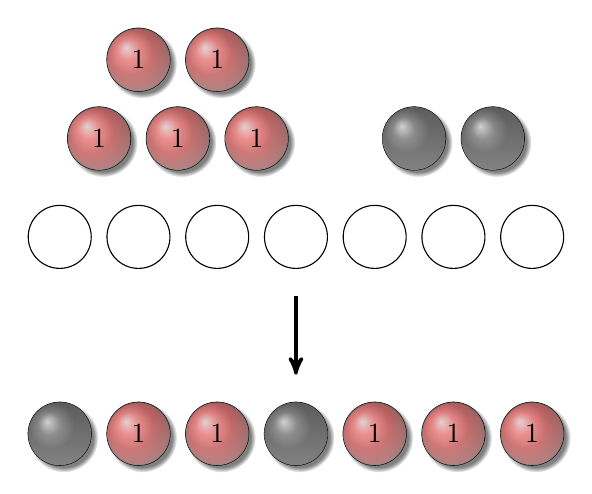
\begin{tikzpicture}
\shade[draw=black, ball color=red, circular drop shadow] (0.5,1.25) circle (4mm);
\shade[fill=white, fill opacity=0.3] (0.5,1.25) circle (4mm) node[fill opacity=1]{1};
\shade[draw=black, ball color=red, circular drop shadow] (1.5,1.25) circle (4mm);
\shade[fill=white, fill opacity=0.3] (1.5,1.25) circle (4mm) node[fill opacity=1]{1};
\shade[draw=black, ball color=red, circular drop shadow] (2.5,1.25) circle (4mm);
\shade[fill=white, fill opacity=0.3] (2.5,1.25) circle (4mm) node[fill opacity=1]{1};
\shade[draw=black, ball color=red, circular drop shadow] (1,2.25) circle (4mm);
\shade[fill=white, fill opacity=0.3] (1,2.25) circle (4mm) node[fill opacity=1]{1};
\shade[draw=black, ball color=red, circular drop shadow] (2,2.25) circle (4mm);
\shade[fill=white, fill opacity=0.3] (2,2.25) circle (4mm) node[fill opacity=1]{1};

\shade[draw=black, ball color=black, circular drop shadow] (4.5,1.25) circle (4mm);
\shade[fill=white, fill opacity=0.3] (4.5,1.25) circle (4mm) node[fill opacity=1]{};
\shade[draw=black, ball color=black, circular drop shadow] (5.5,1.25) circle (4mm);
\shade[fill=white, fill opacity=0.3] (5.5,1.25) circle (4mm) node[fill opacity=1]{};

\draw[draw=black] (0,0) circle (4mm);
\draw[draw=black] (1,0) circle (4mm);
\draw[draw=black] (2,0) circle (4mm);
\draw[draw=black] (3,0) circle (4mm);
\draw[draw=black] (4,0) circle (4mm);
\draw[draw=black] (5,0) circle (4mm);
\draw[draw=black] (6,0) circle (4mm);

\draw[very thick, ->, >=stealth'] (3,-0.75) -- (3,-1.75);

\shade[draw=black, ball color=black, circular drop shadow] (0,-2.5) circle (4mm);
\shade[fill=white, fill opacity=0.3] (0,-2.5) circle (4mm) node[fill opacity=1]{};
\shade[draw=black, ball color=red, circular drop shadow] (1,-2.5) circle (4mm);
\shade[fill=white, fill opacity=0.3] (1,-2.5) circle (4mm) node[fill opacity=1]{1};
\shade[draw=black, ball color=red, circular drop shadow] (2,-2.5) circle (4mm);
\shade[fill=white, fill opacity=0.3] (2,-2.5) circle (4mm) node[fill opacity=1]{1};
\shade[draw=black, ball color=black, circular drop shadow] (3,-2.5) circle (4mm);
\shade[fill=white, fill opacity=0.3] (3,-2.5) circle (4mm) node[fill opacity=1]{};
\shade[draw=black, ball color=red, circular drop shadow] (4,-2.5) circle (4mm);
\shade[fill=white, fill opacity=0.3] (4,-2.5) circle (4mm) node[fill opacity=1]{1};
\shade[draw=black, ball color=red, circular drop shadow] (5,-2.5) circle (4mm);
\shade[fill=white, fill opacity=0.3] (5,-2.5) circle (4mm) node[fill opacity=1]{1};
\shade[draw=black, ball color=red, circular drop shadow] (6,-2.5) circle (4mm);
\shade[fill=white, fill opacity=0.3] (6,-2.5) circle (4mm) node[fill opacity=1]{1};
\end{tikzpicture}
\end{footnotesize}
\caption{The number of possible cardinality assignments for the partition of a set of $n$ elements into $r$ distinct subsets is equivalent to the number of ways to select $n$ positions out of $n + r - 1$ candidates.} 
\label{figure:Partitioning}
\end{center}
\end{figure}

The number of objects in the first subset corresponds to the number of balls appearing before the first marker.
Similarly, the number of objects in the $i$th subset is equal to the number of balls positioned between the $i$th marker and the preceding one.
Finally, the number of objects in the last subset is simply the number of balls after the last marker.
In this scheme, two consecutive markers imply that the corresponding subset is empty.
For example, the integer assignment associated with the Figure~\ref{figure:Partitioning} is
\begin{equation*}
(n_1, n_2, n_3) = (0,2,3).
\end{equation*}

\begin{figure}[htb!]
\begin{center}
% FIGURE GROUP = BALLS
\begin{footnotesize}
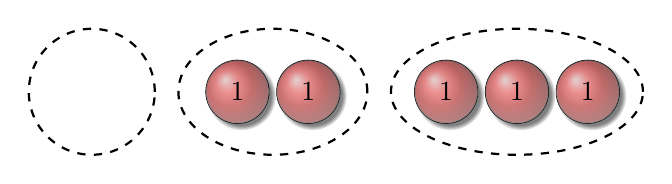
\begin{tikzpicture}
\draw[color=black, thick, dashed] (0,0) circle (8mm);

\draw[color=black, thick, dashed] (2.3,0) ellipse (12mm and 8mm);
\shade[draw=black, ball color=red, circular drop shadow] (1.85,0) circle (4mm);
\shade[fill=white, fill opacity=0.3] (1.85,0) circle (4mm) node[fill opacity=1]{1};
\shade[draw=black, ball color=red, circular drop shadow] (2.75,0) circle (4mm);
\shade[fill=white, fill opacity=0.3] (2.75,0) circle (4mm) node[fill opacity=1]{1};

\draw[color=black, thick, dashed] (5.4,0) ellipse (16mm and 8mm);
\shade[draw=black, ball color=red, circular drop shadow] (4.5,0) circle (4mm);
\shade[fill=white, fill opacity=0.3] (4.5,0) circle (4mm) node[fill opacity=1]{1};
\shade[draw=black, ball color=red, circular drop shadow] (5.4,0) circle (4mm);
\shade[fill=white, fill opacity=0.3] (5.4,0) circle (4mm) node[fill opacity=1]{1};
\shade[draw=black, ball color=red, circular drop shadow] (6.3,0) circle (4mm);
\shade[fill=white, fill opacity=0.3] (6.3,0) circle (4mm) node[fill opacity=1]{1};
\end{tikzpicture}
\end{footnotesize}
\caption{The assignment displayed in Figure~\ref{figure:Partitioning} corresponds to having no element in the first set, two elements in the second set and three elements in the last one.}
\label{figure:Partitioning2}
\end{center}
\end{figure}

There is a natural relation between an integer assignment and the graphical representation depicted above.
To count the number of possible integer assignments, it suffices to calculate the number of ways to place the markers and the balls.
In particular, there are $n + r - 1$ positions, $n$ balls and $r - 1$ markers.
The number of ways to assign the markers is equal to the number of $n$-combinations of $n + r - 1$ elements,
\begin{equation*}
\binom{n + r - 1}{n} = \binom{n + r - 1}{r - 1} .
\end{equation*}

\begin{example}[Sampling with Replacement, without Ordering]
An urn contains $r$ balls numbered one through $r$.
A ball is drawn from the urn and its number is recorded.
The ball is then returned to the urn.
This procedure is repeated a total of $n$ times.
The outcome of this experiment is a table that contains the number of times each ball has come in sight.
We are interested in computing the number of possible outcomes.
This is equivalent to counting the ways a set with $n$ elements can be partitioned into $r$ subsets.
The number of possible outcomes is therefore given by
\begin{equation*}
\binom{n + r - 1}{n} = \binom{n + r - 1}{r - 1} .
\end{equation*}
\end{example}


\section{Combinatorial Examples}

In this section, we present a few applications of combinatorics to computing the probabilities of specific events.

\begin{example}[Pick 3 Texas Lottery]
The Texas Lottery game ``Pick $3$'' is easy to play.
A player must pick three numbers from zero to nine, and choose how to play them: exact order or any order.
The Pick $3$ balls are drawn using three air-driven machines.
These machines employ compressed air to mix and select each ball.

The probability of winning when playing the exact order is
\begin{equation*}
\frac{1}{10} \frac{1}{10} \frac{1}{10}
= \frac{1}{1000} .
\end{equation*}
The probability of winning while playing any order depends on the numbers selected.
When three distinct numbers are selected, the probability of winning is given by
\begin{equation*}
\frac{3!}{1000} = \frac{3}{500} .
\end{equation*}
If a number is repeated twice, the probability of winning becomes
\begin{equation*}
\frac{\binom{3}{2}}{1000} = \frac{3}{1000} .
\end{equation*}
Finally, if a same number is selected three times, the probability of winning decreases to $1/1000$.
\end{example}

\begin{example}[Mega Millions Texas Lottery]
To play the Mega Millions game, a player must select five numbers from $1$ to $56$ in the upper white play area of the play board, and one Mega Ball number from $1$ to $46$ in the lower yellow play area of the play board.
All drawing equipment is stored in a secured on-site storage room.
Only authorized drawings department personnel have keys to the door.
Upon entry of the secured room to begin the drawing process, a lottery drawing specialist examines the security seal to determine if any unauthorized access has occurred.
For each drawing, the Lotto Texas balls are mixed by four acrylic mixing paddles rotating clockwise.
High speed is used for mixing and low speed for ball selection.
As each ball is selected, it rolls down a chute into an official number display area.
We wish to compute the probability of winning the Mega Millions Grand Prize, which requires the correct selection of the five white balls plus the gold Mega ball.

The probability of winning the Mega Millions Grand Prize is
\begin{equation*}
\frac{1}{\binom{56}{5}} \frac{1}{46}
= \frac{51!5!}{56!} \frac{1}{46}
= \frac{1}{175 711 536} .
\end{equation*}
\end{example}

\begin{example}[Sinking Boat]
Six couples, twelve people total, are out at sea on a sail boat.
Unfortunately, the boat hits an iceberg and starts sinking slowly.
Two Coast Guard vessels, the Ibis and the Mako, come to the rescue.
Each boat can rescue six people.
What is the probability that no two people from a same couple end up on the Mako?

Suppose that rescued passengers are assigned to the Ibis and the Mako  at random.
Then, the number of possible ways to partition these passengers between the two vessels is
\begin{equation*}
\binom{12}{6} = \frac{12!}{6! 6!} .
\end{equation*}
If no two people from a same couple end up on the Mako, then each couple is split between the two vessels.
In these circumstances, there are two possibilities for every couple and, using the counting principle, we gather that there are $2^6$ such assignments.
Collecting these results, we conclude that the probability that no two people from a same couple end up on the Mako is equal to
\begin{equation*}
\frac{2^6}{\binom{12}{6}} = \frac{2^6 6! 6!}{12!} .
\end{equation*}
\end{example}


\section*{Further Reading}

\begin{small}
\begin{enumerate}
\item Ross, S., \emph{A First Course in Probability}, 7th edition, Pearson Prentice Hall, 2006: Chapter~1.
\item Bertsekas, D. P., and Tsitsiklis, J. N., \emph{Introduction to Probability}, Athena Scientific, 2002: Section~1.6.
\item Gubner, J. A., \emph{Probability and Random Processes for Electrical and Computer Engineers}, Cambridge, 2006: Section~1.7.
\end{enumerate}
\end{small}

 % No psfrags
\chapter{Basic Concepts of Probability}

The theory of probability provides the mathematical tools necessary to study and analyze uncertain phenomena that occur in nature.
It establishes a formal framework to understand and predict the outcome of a random experiment.
It can be used to model complex systems and characterize stochastic processes.
This is instrumental in designing efficient solutions to many engineering problems.
Two components define a probabilistic model, a sample space and a probability law.

%%%% COMMENT
% Sample Space: What questions can be asked?
% Probability Law: What are the answers?

\section{Sample Spaces and Events}

In the context of probability, an \emph{experiment} is a random occurrence that produces one of several \emph{outcomes}.\index{Experiment}\index{Outcome}
The set of all possible outcomes is called the \emph{sample space} of the experiment, and it is denoted by $\Omega$.\index{Sample space}
An \emph{admissible} subset of the sample space is called an \emph{event}.\index{Event}

\begin{figure}[htb!]
\begin{center}
% FIGURE GROUP = BALLS
\begin{footnotesize}
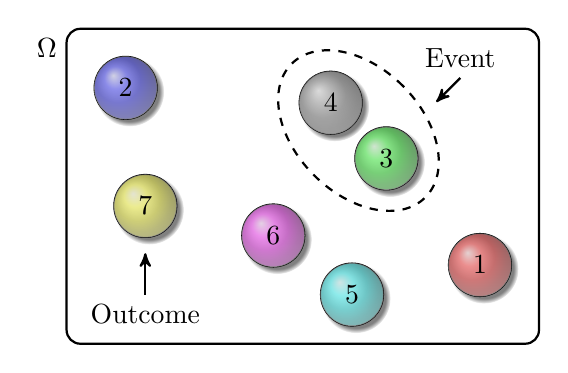
\begin{tikzpicture}
\draw[color=black, thick, rounded corners=5] (-3,-2) rectangle (3,2);
\node at (-3.25,1.75) {$\Omega$};

\draw[color=black, thick, dashed, rotate=45] (1,0) ellipse (8mm and 12mm);

\shade[draw=black, ball color=red, circular drop shadow] (2.25,-1) circle (4mm);
\shade[fill=white, fill opacity=0.3] (2.25,-1) circle (4mm) node[fill opacity=1]{1};

\shade[draw=black, ball color=blue, circular drop shadow] (-2.25,1.25) circle (4mm);
\shade[fill=white, fill opacity=0.3] (-2.25,1.25) circle (4mm) node[fill opacity=1]{2};

\shade[draw=black, ball color=green, circular drop shadow] (1.061,0.354) circle (4mm);
\shade[fill=white, fill opacity=0.3] (1.061,0.354) circle (4mm) node[fill opacity=1]{3};

\shade[draw=black, ball color=gray, circular drop shadow] (0.354,1.061) circle (4mm);
\shade[fill=white, fill opacity=0.3] (0.354,1.061) circle (4mm) node[fill opacity=1]{4};

\shade[draw=black, ball color=cyan, circular drop shadow] (0.625,-1.375) circle (4mm);
\shade[fill=white, fill opacity=0.3] (0.625,-1.375) circle (4mm) node[fill opacity=1]{5};

\shade[draw=black, ball color=magenta, circular drop shadow] (-0.375,-0.625) circle (4mm);
\shade[fill=white, fill opacity=0.3] (-0.375,-0.625) circle (4mm) node[fill opacity=1]{6};

\shade[draw=black, ball color=yellow, circular drop shadow] (-2,-0.25) circle (4mm);
\shade[fill=white, fill opacity=0.3] (-2,-0.25) circle (4mm) node[fill opacity=1]{7};
\node at (-2,-1.625) {Outcome};
\draw [thick, ->, >=stealth', shorten >= 1mm] (-2,-1.375) -- (-2,-0.75);

\node at (2,1.625) {Event};
\draw [thick, ->, >=stealth', shorten >= 1mm] (2,1.375) -- (1.625,1);
\end{tikzpicture}
\end{footnotesize}
\caption{A sample space contains all the possible outcomes; an admissible subset of the sample space is called an event.}
\label{figure:SampleSpace}
\end{center}
\end{figure}

\begin{example}
The rolling of a die forms a common experiment.
A sample space $\Omega$ corresponding to this experiment is given by the six faces of a die.
The set of prime numbers less than or equal to six, namely $\{ 2, 3, 5 \}$, is one of many possible events.
The actual number observed after rolling the die is the outcome of the experiment.

\begin{figure}[htb!]
\begin{center}
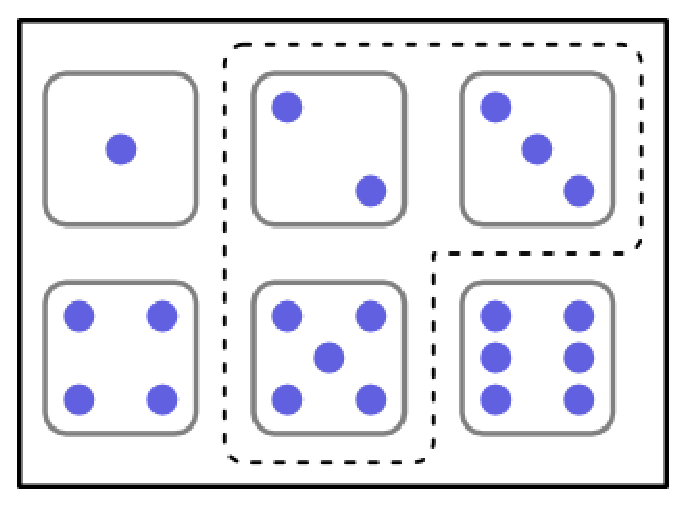
\includegraphics[height=3.38cm]{Figures/2Chapter/dices}
\caption{A possible sample space for the rolling of a die is $\Omega = \{ 1, 2, \ldots, 6 \}$, and the subset $\{2, 3, 5 \}$ forms a specific event.}
\end{center}
\end{figure}
\end{example}

There is essentially no restriction on what constitutes an experiment.
The flipping of a coin, the flipping of $n$ coins, and the tossing of an infinite sequence of coins are all random experiments.
Also, two similar experiments may have different sample spaces.
A sample space $\Omega$ for observing the number of heads in $n$ tosses of a coin is $\{ 0, 1, \ldots, n \}$; however, when describing the complete history of the $n$ coin tosses, the sample space becomes much larger with $2^n$ distinct sequences of heads and tails.
Ultimately, the choice of a particular sample space depends on the properties one wishes to analyze.
Yet some rules must be followed in selecting a sample space.
\begin{enumerate}
%%%% COMMENT
% Uniqueness
\item The elements of a sample space should be \emph{distinct} and \emph{mutually exclusive}.
This ensures that the outcome of an experiment is unique.\index{Distinct elements}\index{Mutually exclusive}
%%%% COMMENT
% Existence
\item A sample space must be \emph{collectively exhaustive}.
That is, every possible outcome of the experiment must be accounted for in the sample space.\index{Collectively exhaustive}
\end{enumerate}
In general, a sample space should be precise enough to distinguish between all outcomes of interest, while avoiding frivolous details.

\begin{example}
Consider the space composed of the odd integers located between one and six, the even integers contained between one and six, and the prime numbers less than or equal to six.
This collection cannot be a sample space for the rolling of a die because its elements are not mutually exclusive.
In particular, the numbers three and five are both odd and prime, while the number two is prime and even.
This violates the uniqueness criterion.

\begin{figure}[htb!]
\begin{center}
\includegraphics[height=4.125cm]{Figures/2Chapter/nonadmissiblespace}
\caption{This collection of objects cannot be a sample space as the three proposed outcomes (even, odd and prime) are not mutually exclusive.}
\end{center}
\end{figure}

Alternatively, the elements of the space composed of the odd numbers between one and six, and the even numbers between one and six, are distinct and mutually exclusive;
an integer cannot be simultaneously odd and even.
Moreover, this space is collectively exhaustive because every integer is either odd or even.
This latter description forms a possible sample space for the rolling of a die.

\begin{figure}[htb!]
\begin{center}
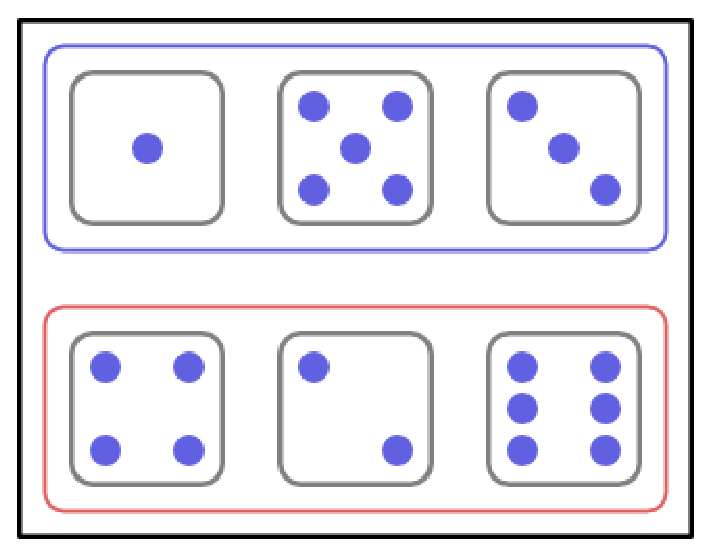
\includegraphics[height=3.75cm]{Figures/2Chapter/admissiblespace}
\end{center}
\caption{A candidate sample space for the rolling of a die is composed of two objects, the odd numbers and the even numbers between one and six.}
\end{figure}
\end{example}


\section{Probability Laws}
\label{section:ProbabilityLaws}

A \emph{probability law} specifies the likelihood of events related to an experiment.\index{Probability law}
Formally, a probability law assigns to every event $A$ a number $\Pr (A)$, called the \emph{probability of event $A$}, such that the following axioms are satisfied.
\begin{enumerate}
\item \textbf{(Nonnegativity)} $\Pr (A) \geq 0$, for every event $A$.
\item \textbf{(Normalization)} The probability of the sample space $\Omega$ is equal to one,
\begin{equation*}
\Pr (\Omega) = 1 .
\end{equation*}
\item \textbf{(Countable Additivity)} If $A$ and $B$ are disjoint events, $A \cap B = \emptyset$, then the probability of their union satisfies
\begin{equation*}
\Pr (A \cup B) = \Pr (A) + \Pr (B) .
\end{equation*}
More generally, if $A_1, A_2, \ldots$ is a sequence of disjoint events and $\bigcup_{k=1}^{\infty} A_k$ is itself an admissible event then
\begin{equation*}
\Pr \left( \bigcup_{k=1}^{\infty} A_k \right)
= \sum_{k = 1}^{\infty} \Pr (A_k) .
\end{equation*}
\end{enumerate}

A number of important properties can be deduced from the three axioms of probability.
We prove two such properties below.
The first statement describes the relation between inclusion and probabilities.
\begin{proposition}
If $A \subset B$, then $\Pr (A) \leq \Pr (B)$.
\end{proposition}
\begin{proof}
Since $A \subset B$, we have $B = A \cup (B - A)$.
Noting that $A$ and $B - A$ are disjoint sets, we get
\begin{equation*}
\Pr (B) = \Pr (A) + \Pr (B - A) \geq \Pr (A) ,
\end{equation*}
where the inequality follows from the nonnegativity of probability laws.
\end{proof}
\begin{figure}[htb!]
\begin{center}
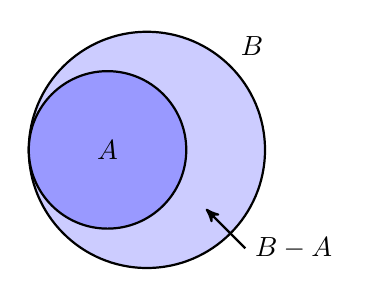
\begin{tikzpicture}
\node[circle,draw=black,thick,fill=blue!20,minimum size=3cm,label=45:$B$] (B) at (0,0) {};
\node[circle,draw=black,thick,fill=blue!40,minimum size=2cm] (A) at (-0.5cm,0) {$A$};
\coordinate [label=right:{$B - A$}] (Difference) at (1.25cm,-1.25cm);
\draw[->,thick,>=stealth'] (Difference) to (0.75cm,-0.75cm);
\end{tikzpicture}
\caption{If event $A$ is a subset of event $B$, then the probability of $A$ is less than or equal to the probability of $B$.}
\end{center}
\end{figure}

Our second result specifies the probability of the union of two events that are not necessarily mutually exclusive.
\begin{proposition} \label{proposition:ProbabilityUnion}
$\Pr (A \cup B) = \Pr (A) + \Pr (B) - \Pr (A \cap B)$.
\end{proposition}
\begin{proof}
Using the third axiom of probability on the disjoint sets $A$ and $(A \cup B) - A$, we can write
\begin{equation*}
\Pr (A \cup B)
= \Pr (A) + \Pr ((A \cup B) - A)
= \Pr (A) + \Pr (B - A) .
\end{equation*}
Similarly, applying the third axiom to $A \cap B$ and $B - (A \cap B)$, we obtain
\begin{equation*}
\Pr (B)
= \Pr (A \cap B) + \Pr (B - (A \cap B))
= \Pr (A \cap B) + \Pr (B - A) .
\end{equation*}
Combining these two equations yields the desired result.
\end{proof}
\begin{figure}[htb!]
\begin{center}
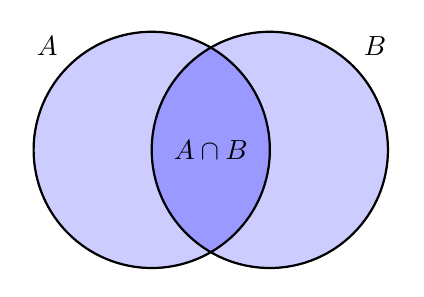
\begin{tikzpicture}
\draw[fill=blue!20]
    (-0.75cm,0) circle (1.5cm)
    (0.75cm,0) circle (1.5cm);
\begin{scope}
    \clip (-0.75cm,0) circle (1.5cm);
    \fill[fill=blue!40] (0.75cm,0) circle (1.5cm);
\end{scope}
\node[circle,draw=black,thick,minimum size=3cm,label=135:$A$] (A) at (-0.75cm,0) {};
\node[circle,draw=black,thick,minimum size=3cm,label=45:$B$] (B) at (0.75cm,0) {};
\coordinate [label=center:{$A \cap B$}] (Intersection) at (0,0);
\end{tikzpicture}
\caption{The probability of the union of $A$ and $B$ is equal to the probability of $A$ plus the probability of $B$ minus the probability of their intersection.}
\end{center}
\end{figure}

The statement of Proposition~\ref{proposition:ProbabilityUnion} can be extended to finite unions of events.
Specifically, we can write
\begin{equation*}
\Pr \left( \bigcup_{k=1}^{n} A_k \right)
= \sum_{k = 1}^{n} (-1)^{k-1} \sum_{\IndexSet \subset \{1, \ldots, n \}, |\IndexSet| =k } \Pr \left( \bigcap_{i \in \IndexSet} A_i \right)
\end{equation*}
where the rightmost sum runs over all subsets $\IndexSet$ of $\{ 1, \ldots, n \}$ that contain exactly $k$ elements.
This more encompassing result is known as the \emph{inclusion-exclusion principle}.\index{Inclusion-exclusion principle}

We can use Proposition~\ref{proposition:ProbabilityUnion} recursively to derive a bound on the probabilities of unions.
This theorem, which is sometimes called the \emph{Boole inequality}, asserts that the probability of at least one event occurring is no greater than the sum of the probabilities of the individual events.\index{Boole inequality}

\begin{theorem}[Union Bound]\index{Union bound}
Let $A_1, A_2, \ldots, A_n$ be a collection of events, then
\begin{equation} \label{equation:UnionBound}
\Pr \left( \bigcup_{k=1}^n A_k \right)
\leq \sum_{k=1}^n \Pr (A_k) .
\end{equation}
\end{theorem}
\begin{proof}
We show this result using induction.
First, we note that the claim is trivially true for $n = 1$.
As an inductive hypothesis, assume that \eqref{equation:UnionBound} holds for some $n \geq 1$.
Then, we have
\begin{equation*}
\begin{split}
\Pr \left( \bigcup_{k=1}^{n+1} A_k \right)
&= \Pr \left( A_{n+1} \cup \left( \bigcup_{k=1}^{n} A_k \right) \right) \\
&= \Pr (A_{n+1}) + \Pr \left( \bigcup_{k=1}^{n} A_k \right)
- \Pr \left( A_{n+1} \cap \left( \bigcup_{k=1}^{n} A_k \right) \right) \\
&\leq \Pr (A_{n+1}) + \Pr \left( \bigcup_{k=1}^{n} A_k \right)
\leq \sum_{k = 1}^{n+1} \Pr (A_k) .
\end{split}
\end{equation*}
Therefore, by the principle of mathematical induction, \eqref{equation:UnionBound} is valid for all positive integers.
\end{proof}

The union bound is often employed in situations where finding the joint probability of multiple rare events is difficult, but computing the probabilities of the individual components is straightforward. 

\begin{example}
An urn contains 990 blue balls and 10 red balls.
Five people each pick a ball at random, without replacement.
We wish to compute the probability that at least one person picks a red ball.
Let $B_k$ denote the event that person~$k$ draws a red ball.
We note that the probability of interest can be written as $\Pr \left( \bigcup_{k=1}^5 B_k \right)$.

First, let us approximate this probability using the union bound.
Clearly, the probability that the first person picks a red ball, $\Pr (B_1)$, is equal to 1/100.
As we will see later, it turns out that $\Pr (B_k) = 1/100$ for $k=1,\ldots,5$.
Applying \eqref{equation:UnionBound}, we get a bound on the probability that at least one person picks a red ball,
\begin{equation*}
\Pr \left( \bigcup_{k=1}^5 B_k \right)
\leq \sum_{k=1}^5 \Pr ( B_k )
= \sum_{k=1}^5 \frac{1}{100} = \frac{1}{20} .
\end{equation*}
We can also compute this probability exactly.
The probability that no red balls are selected is given by $\binom{990}{5} / \binom{1000}{5}$.
Hence, the probability that a least one person draws a red ball becomes
\begin{equation*}
\Pr \left( \bigcup_{k=1}^5 B_k \right)
= 1 - \frac{\binom{990}{5}}{\binom{1000}{5}}
\approx 0.0491 .
\end{equation*}

As a second application, consider the problem where the five people each draw two balls from the urn, without replacement.
This time, we wish to approximate the probability that at least one person gets two red balls.
Using the same steps as before, we get
\begin{equation*}
\Pr \left( \bigcup_{k=1}^5 C_k \right)
\leq \sum_{k=1}^5 \Pr ( C_k )
= \sum_{k=1}^5 \frac{\binom{10}{2}}{\binom{1000}{2}} = \frac{1}{2220} ,
\end{equation*}
where $C_k$ represents the event that person $k$ draws two red balls.
In this latter scenario, computing the exact probability is much more challenging.
\end{example}


\subsection{Finite Sample Spaces}
\label{section:FiniteSampleSpaces}

If a sample space $\Omega$ contains a finite number of elements, then a probability law on $\Omega$ is completely determined by the probabilities of its individual outcomes.
Denote a sample space containing $n$ elements by $\Omega = \{ s_1, s_2, \ldots, s_n \}$.
Any event in $\Omega$ is of the form $A = \{ s_i \in \Omega | i \in \IndexSet \}$, where $\IndexSet$ is a subset of the integers one through $n$.
The probability of event $A$ is therefore given by the third axiom of probability,
\begin{equation*}
\Pr (A)
= \Pr ( \{ s_i \in \Omega | i \in \IndexSet \} )
= \sum_{i \in \IndexSet} \Pr (s_i) .
\end{equation*}
We emphasize that, by definition, distinct outcomes are always disjoint events.

If in addition the elements of $\Omega$ are equally likely with
\begin{equation*}
\Pr (s_1) = \Pr (s_2) = \cdots = \Pr (s_n) = \frac{1}{n} ,
\end{equation*}
then the probability of an event $A$ becomes
\begin{equation} \label{equation:ProbEquiProbableOutcomes}
\Pr (A) = \frac{ |A| }{n}
\end{equation}
where $|A|$ denotes the number of elements in $A$.

\begin{example}
The rolling of a fair die is an experiment with a finite number of equally likely outcomes.
The probability of observing any of the faces labeled one through six is therefore equal to $1/6$.
The probability of any event can easily be computed by counting the number of distinct outcomes included in the event.
For instance, the probability of rolling a prime number is
\begin{equation*}
\Pr ( \{ 2, 3, 5 \} )
= \Pr (2) + \Pr(3) + \Pr(5) = \frac{3}{6} .
\end{equation*}
\end{example}


\subsection{Countably Infinite Models}

Consider a sample space that consists of a countably infinite number of elements, $\Omega = \{ s_1, s_2, \ldots \}$.
Again, a probability law on $\Omega$ is specified by the probabilities of individual outcomes.
An event in $\Omega$ can be written as $A = \{ s_j \in \Omega | j \in \JndexSet \}$, where $\JndexSet$ is a subset of the positive integers.
Using the third axiom of probability, $\Pr (A)$ can be written as
\begin{equation*}
\Pr (A)
= \Pr ( \{ s_j \in \Omega | j \in \JndexSet \} )
= \sum_{j \in \JndexSet} \Pr (s_j) .
\end{equation*}
The possibly infinite sum $\sum_{j \in \JndexSet} \Pr (s_j)$ always converges since the summands are nonnegative and the sum is bounded above by one; it is consequently well defined.

\begin{figure}[htb!]
\begin{center}
% FIGURE GROUP = BALLS
\begin{footnotesize}
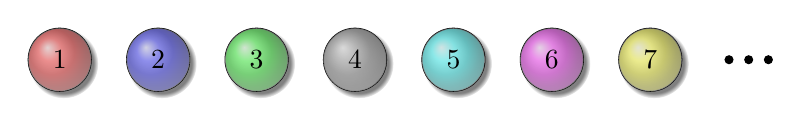
\begin{tikzpicture}
\shade[draw=black, ball color=red, circular drop shadow] (0,0) circle (4mm);
\shade[fill=white, fill opacity=0.3] (0,0) circle (4mm) node[fill opacity=1]{1};

\shade[draw=black, ball color=blue, circular drop shadow] (1.25,0) circle (4mm);
\shade[fill=white, fill opacity=0.3] (1.25,0) circle (4mm) node[fill opacity=1]{2};

\shade[draw=black, ball color=green, circular drop shadow] (2.5,0) circle (4mm);
\shade[fill=white, fill opacity=0.3] (2.5,0) circle (4mm) node[fill opacity=1]{3};

\shade[draw=black, ball color=gray, circular drop shadow] (3.75,0) circle (4mm);
\shade[fill=white, fill opacity=0.3] (3.75,0) circle (4mm) node[fill opacity=1]{4};

\shade[draw=black, ball color=cyan, circular drop shadow] (5,0) circle (4mm);
\shade[fill=white, fill opacity=0.3] (5,0) circle (4mm) node[fill opacity=1]{5};

\shade[draw=black, ball color=magenta, circular drop shadow] (6.25,0) circle (4mm);
\shade[fill=white, fill opacity=0.3] (6.25,0) circle (4mm) node[fill opacity=1]{6};

\shade[draw=black, ball color=yellow, circular drop shadow] (7.5,0) circle (4mm);
\shade[fill=white, fill opacity=0.3] (7.5,0) circle (4mm) node[fill opacity=1]{7};

\draw[draw=black, fill=black] (8.5,0) circle (0.5mm);
\draw[draw=black, fill=black] (8.75,0) circle (0.5mm);
\draw[draw=black, fill=black] (9,0) circle (0.5mm);
\end{tikzpicture}
\end{footnotesize}
\caption{A countable set is a collection of elements with the same cardinality as some subset of the natural numbers.}
\end{center}
\end{figure}

\begin{example} \label{example:CoinTossSequence}
Suppose that a fair coin is tossed repetitively until heads is observed.
The number of coin tosses is recorded as the outcome of this experiment.
A natural sample space for this experiment is $\Omega = \{ 1, 2, \ldots \}$, a countably infinite set.

The probability of observing heads on the first trial is $1/2$, and the probability of observing heads for the first time on trial $k$ is $2^{-k}$.
The probability of the entire sample space is therefore equal to
\begin{equation*}
\Pr ( \Omega ) = \sum_{k=1}^{\infty} \Pr (k)
= \sum_{k=1}^{\infty} \frac{1}{2^k} = 1 ,
\end{equation*}
as expected.
Similarly, the probability of the number of coin tosses being even can be computed as
\begin{equation*}
\Pr ( \{ 2, 4, 6, \ldots \} )
= \sum_{k=1}^{\infty} \Pr (2k)
= \sum_{k = 1}^{\infty} \frac{1}{2^{2k}}
= \frac{1}{4} \frac{1}{ \left( 1 - \frac{1}{4} \right) }
= \frac{1}{3} .
\end{equation*}
\end{example}


\subsection{Uncountably Infinite Models}

Probabilistic models with uncountably infinite sample spaces differ from the finite and countable cases in that a probability law may not necessarily be specified by the probabilities of single-element outcomes.
This difficulty arises from the large number of elements contained in the sample space when the latter is uncountable.
Many subsets of $\Omega$ do not have a finite or countable representation, and as such the third axiom of probability cannot be applied to relate the probabilities of these events to the probabilities of individual outcomes.
Despite these apparent difficulties, probabilistic models with uncountably infinite sample spaces are quite useful in practice.
To develop an understanding of uncountable probabilistic models, we consider the unit interval $[0, 1]$.

\begin{figure}[htb!]
\begin{center}
\begin{psfrags}
\psfrag{0}[c]{$0$}
\psfrag{1}[c]{$1$}
\includegraphics[height=1.17cm]{Figures/2Chapter/uncountablespace}
\end{psfrags}
\caption{The unit interval $[0,1]$, composed of all real numbers between zero and one, is an example of an uncountable set.}
\end{center}
\end{figure}

Suppose that an element is chosen at random from this interval, with uniform weighting.
By the first axiom of probability, the probability that this element belongs to the interval $[0,1]$ is given by $\Pr \left( [0,1] \right) = 1$.
Furthermore, if two intervals have the same length, the probabilities of the outcome falling in either interval should be identical.
For instance, it is natural to anticipate that $\Pr \left( \left( 0, 0.25 \right) \right) = \Pr \left( \left( 0.75, 1 \right) \right)$.

\begin{figure}[htb!]
\begin{center}
\begin{psfrags}
\psfrag{0}[l]{$0$}
\psfrag{0.25}[r]{$0.25$}
\psfrag{0.75}[l]{$0.75$}
\psfrag{1}[r]{$1$}
\includegraphics[height=1.185cm]{Figures/2Chapter/intervals}
\end{psfrags}
\caption{If the outcome of an experiment is uniformly distributed over $[0,1]$, then two subintervals of equal lengths should have the same probabilities.}
\end{center}
\end{figure}

In an extension of the previous observation, we take the probability of an open interval $(a, b)$ where $0 \leq a < b \leq 1$ to equal
\begin{equation} \label{equation:DefinitionProbabilityLaw1}
\Pr ( (a,b) ) = b - a .
\end{equation}
Using the third axiom of probability, it is then possible to find the probability of a finite or countable union of disjoint open intervals.

\begin{figure}[htb!]
\begin{center}
\begin{psfrags}
\psfrag{0}[l]{$0$}
\psfrag{1}[r]{$1$}
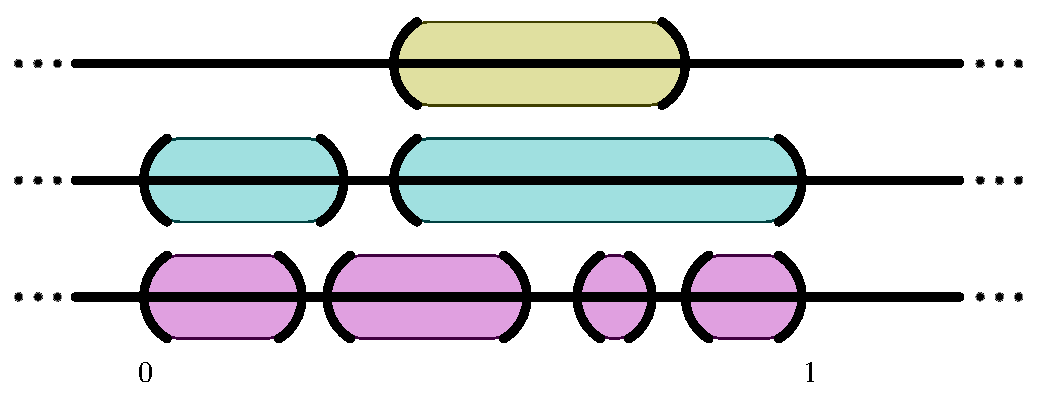
\includegraphics[height=3.28cm]{Figures/2Chapter/lineintervals}
\end{psfrags}
\caption{The probabilities of events that are formed through the union of disjoint intervals can be computed in a straightforward manner.}
\end{center}
\end{figure}

Specifically, for constants $0 \leq a_1 < b_1 < a_2 < b_2 < \cdots \leq 1$, we get
\begin{equation*}
\Pr \left( \bigcup_{k=1}^{\infty} (a_k,b_k) \right)
= \sum_{k=1}^{\infty} \left( b_k - a_k \right) .
\end{equation*}
The probabilities of more complex events can be obtained by applying additional elementary set operations.
However, it suffices to say for now that specifying the probability of the outcome falling in $(a,b)$ for every possible open interval is enough to define a probability law on $\Omega$.
In the example at hand, \eqref{equation:DefinitionProbabilityLaw1} completely determines the probability law on $[0,1]$.

Note that we can give an alternative means of computing the probability of an interval.
Again, consider the open interval $(a, b)$ where $0 \leq a < b \leq 1$.
The probability of the outcome falling in this  interval is equal to
\begin{equation*}
\Pr ( (a, b) ) = b - a = \int_a^b dx = \int_{(a,b)} dx .
\end{equation*}
Moreover, for $0 \leq a_1 < b_1 < a_2 < b_2 < \cdots \leq 1$, we can write
\begin{equation*}
\Pr \left( \bigcup_{k=1}^{\infty} (a_k,b_k) \right)
= \sum_{k=1}^{\infty} \left( b_k - a_k \right)
= \int_{\bigcup_{k=1}^{\infty} (a_k,b_k)} dx .
\end{equation*}
For this carefully crafted example, it appears that the probability of an admissible event $A$ is given by the integral
\begin{equation*}
\Pr (A) = \int_{A} dx .
\end{equation*}
This is indeed accurate for the current scenario.
In fact, the class of admissible events for this experiment is simply the collection of all sets for which the integral $\int_A dx$ can be computed.
In other words, if a number is chosen at random from $[0,1]$, then the probability of this number falling in set $A \subset [0,1]$ is
\begin{equation*}
\Pr (A) = \int_{A} dx .
\end{equation*}
This method of computing probabilities can be extended to more complicated problems.
In these notes, we will see many probabilistic models with uncountably infinite sample spaces.
The mathematical tools required to handle such models will be treated alongside.

\begin{example}
Suppose that a participant at a game-show is required to spin the wheel of serendipity, a perfect circle with unit radius.
When subjected to a vigorous spin, the wheel is equally likely to stop anywhere along its perimeter.
A sampling space for this experiment is the collection of all angles from $0$ to $2 \pi$, an uncountable set.
The probability of $\Omega$ is invariably equal to one, $\Pr ([0, 2 \pi)) = 1$.

\begin{figure}[tbh!]
\begin{center}
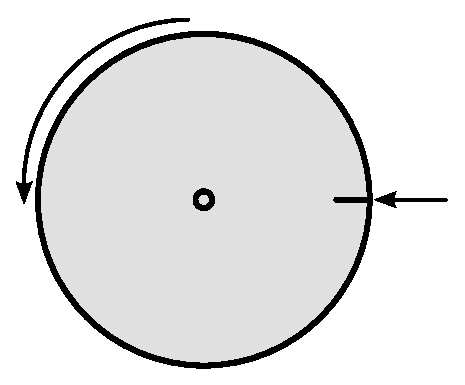
\includegraphics[height=3.15cm]{Figures/2Chapter/wheel}
\caption{The wheel of serendipity forms an example of a random experiment for which the sample space is uncountable.}
\end{center}
\end{figure}

The probability that the wheel stops in the first quadrant is given by
\begin{equation*}
\Pr \left( \left[ 0, \frac{\pi}{2} \right) \right)
= \int_{0}^{\frac{\pi}{2}} \frac{1}{2 \pi} d\theta
= \frac{1}{4}.
\end{equation*}
More generally, the probability that the wheel stops in an interval $(a, b)$ where $0 \leq a \leq b < 2 \pi$ can be written as
\begin{equation*}
\Pr ((a,b)) = \frac{b - a}{2 \pi}.
\end{equation*}
If $B \subset [0, 2 \pi)$ is a set representing all winning outcomes, then the probability of success at the wheel becomes
\begin{equation*}
\Pr(B) = \int_B \frac{1}{2 \pi} d\theta .
\end{equation*}
\end{example}


\subsection{Probability and Measure Theory*}

A thorough treatment of probability involves advanced mathematical concepts, especially when it comes to infinite sample spaces.
The basis of our intuition for the infinite is the set of \emph{natural numbers},\index{Natural numbers}
\begin{equation*}
\NaturalNumbers = \{ 1, 2, \ldots \}.
\end{equation*}
Two sets are said to have the same \emph{cardinality} if their elements can be put in one-to-one correspondence.\index{Cardinality}
A set with the same cardinality as a subset of the natural numbers is said to be \emph{countable}.\index{Countable}
That is, the elements of a countable set can always be listed in sequence, $s_1, s_2, \ldots$; although the order may have nothing to do with any relation between the elements.
The integers and the rational numbers are examples of countably infinite sets.
It may be surprising at first to learn that there exist uncountable sets.
To escape beyond the countable, one needs set theoretic tools such as \emph{power sets}.\index{Power set}
The set of real numbers is uncountably infinite; it cannot be put in one-to-one correspondence with the natural numbers.
A typical progression in analysis consists of using the finite to gain intuition about the countably infinite, and then to employ the countably infinite to get at the uncountable.

It is tempting to try to assign probabilities to every subset of a sample space $\Omega$.
However, for uncountably infinite sample spaces, this leads to serious difficulties that cannot be resolved.
In general, it is necessary to work with special subclasses of the class of all subsets of a sample space $\Omega$.
The collections of the appropriate kinds are called fields and $\sigma$-fields, and they are studied in \emph{measure theory}.\index{Measure theory}
This leads to measure-theoretic probability, and to its unified treatment of the discrete and the continuous.

Fortunately, it is possible to develop a working understanding of probability without worrying excessively about these issues.
At some point in your academic career, you may wish to study analysis and measure theory more carefully and in greater details.
However, it is not our current purpose to initiate the rigorous treatment of these topics.


\section*{Further Reading}

\begin{small}
\begin{enumerate}
\item Ross, S., \emph{A First Course in Probability}, 7th edition, Pearson Prentice Hall, 2006: Chapter~2.
\item Bertsekas, D. P., and Tsitsiklis, J. N., \emph{Introduction to Probability}, Athena Scientific, 2002: Section~1.2.
\item Miller, S. L., and Childers, D. G., \emph{Probability and Random Processes with Applications to Signal Processing and Communications}, 2004: Sections~2.1--2.3.
\item Gubner, J. A., \emph{Probability and Random Processes for Electrical and Computer Engineers}, Cambridge, 2006: Sections~1.1,1.3--1.4.
\end{enumerate}
\end{small}


%\chapter{Conditional Probability}
\label{chapter:ConditionalProbability}

Conditional probability provides a way to compute the likelihood of an event based on \emph{partial information}.
This is a powerful concept that is used extensively throughout engineering with applications to decision making, networks, communications and many other fields.


\section{Conditioning on Events}

We begin our description of conditional probability with illustrative examples.
The intuition gained through this exercise is then generalized by introducing a formal definition for this important concept.

\begin{example}
The rolling of a fair die is an experiment with six equally likely outcomes.
As such, the probability of obtaining any of the outcomes is $1/6$.
However, if we are told that the upper face features an odd number, then only three possibilities remain, namely $\{1, 3, 5 \}$.
\begin{figure}[htb!]
\begin{center}
\begin{psfrags}
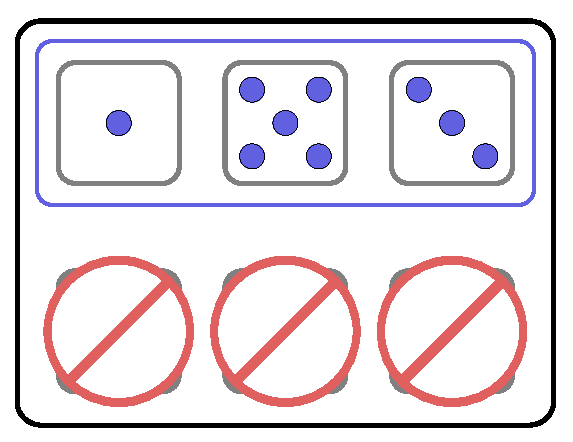
\includegraphics[height=3.675cm]{Figures/3Chapter/condevent}
\end{psfrags}
\caption{Partial information about the outcome of an experiment may change the likelihood of events.
The resulting values are known as conditional probabilities.}
\label{figure:CondEvent}
\end{center}
\end{figure}
These three outcomes had equal probabilities before the additional information was revealed.
It then seems natural to assume that they remain equally likely afterwards.
In particular, it is reasonable to assign a probability of $1/3$ to each of the three outcomes that remain possible candidates after receiving the side information.
We can express the probability of getting a three given that the outcome is an odd number as
\begin{equation*}
\frac{\Pr (3 \cap \{ 1, 3, 5 \})}{\Pr (\{ 1, 3, 5 \} ) }
= \frac{\Pr(3)}{\Pr (\{1,3,5\})} = \frac{1}{3} .
\end{equation*}
\end{example}

\begin{example}
Let $A$ and $B$ be events associated with a random experiment, and assume that $\Pr(B)>0$.
To gain additional insight into conditional probability, we consider the scenario where this experiment is repeated $N$ times.
Let $N_{AB}$ be the number of trials for which $A \cap B$ occurs, $N_{A\overline{B}}$ be the number of times where only $A$ occurs,  $N_{\overline{A}B}$ be the number of times where only $B$ occurs, and  $N_{\overline{A}\overline{B}}$ be the number of trials for which neither takes place.
From these definitions, we gather that $A$ is observed exactly $N_A = N_{AB} + N_{A\overline{B}}$ times, and $B$ is seen $N_B = N_{AB} + N_{\overline{A}B}$ times.

The frequentist view of probability is based on the fact that, as $N$ becomes large, one can approximate the probability of an event by taking the ratio of the number of times this event occurs over the total number of trials.
For instance, we can write
\begin{xalignat*}{2}
\Pr (A\cap B) & \approx \frac{N_{AB}}{N} &
\Pr (B) & \approx \frac{N_{B}}{N}.
\end{xalignat*}
Likewise, the conditional probability of $A$ given knowledge that the outcome lies in $B$ can be computed using
\begin{equation} \label{equation:FrequentistApproximation}
\Pr (A | B) \approx \frac{N_{AB}}{N_B}
= \frac{N_{AB} / N}{N_B / N} \approx \frac{\Pr (A \cap B)}{\Pr (B)}.
\end{equation}
As $N$ approaches infinity, these approximations become exact and \eqref{equation:FrequentistApproximation} unveils the formula for conditional probability.
\end{example}

Having considered intuitive arguments, we turn to the mathematical definition of conditional probability.
Let $B$ be an event such that $\Pr (B) > 0$.
A conditional probability law assigns to every event $A$ a number $\Pr (A|B)$, termed the \emph{conditional probability of $A$ given $B$}, such that \index{Conditional probability}
\begin{equation} \label{equation:ConditionalProbability}
\Pr (A | B) = \frac{\Pr (A \cap B)}{\Pr (B)}.
\end{equation}
We can show that the collection of conditional probabilities $\{ \Pr (A | B) \}$ specifies a valid probability law, as defined in Section~\ref{section:ProbabilityLaws}.
For every event $A$, we have
\begin{equation*}
\Pr (A|B) = \frac{\Pr (A \cap B)}{\Pr (B)} \geq 0
\end{equation*}
and, hence, $\Pr (A|B)$ is nonnegative.
The probability of the entire sample space $\Omega$ is equal to
\begin{equation*}
\Pr (\Omega | B) = \frac{\Pr (\Omega \cap B)}{\Pr (B)}
= \frac{\Pr (B)}{\Pr (B)} = 1 .
\end{equation*}
If $A_1, A_2, \ldots$ is a sequence of disjoint events, then
\begin{equation*}
A_1 \cap B, A_2 \cap B, \ldots
\end{equation*}
is also a sequence of disjoint events and
\begin{equation*}
\begin{split}
\Pr \left( \bigcup_{k=1}^{\infty} A_k \Big| B \right)
&= \frac{\Pr \left( \left( \bigcup_{k=1}^{\infty} A_k \right) \cap B \right)}{\Pr (B)}
= \frac{\Pr \left( \bigcup_{k=1}^{\infty} (A_k \cap B ) \right)}{\Pr (B)} \\
&= \sum_{k = 1}^{\infty} \frac{ \Pr (A_k \cap B ) }{\Pr (B)}
= \sum_{k = 1}^{\infty} \Pr (A_k | B) ,
\end{split}
\end{equation*}
where the third equality follows from the third axiom of probability applied to the set $\bigcup_{k=1}^{\infty} (A_k \cap B )$.
Thus, the conditional probability law defined by \eqref{equation:ConditionalProbability} satisfies the three axioms of probability.

\begin{example}
A fair coin is tossed repetitively until heads is observed.
In Example~\ref{example:CoinTossSequence}, we found that the probability of observing heads for the first time on trial $k$ is $2^{-k}$.
We now wish to compute the probability that heads occurred for the first time on the second trial given that it took an even number of tosses to observe heads.
In this example, $A = \{ 2 \}$ and $B$ is the set of even numbers.
The probability that the outcome is two, given that the number of tosses is even, is equal to
\begin{equation*}
\Pr ( 2 | B )
= \frac{\Pr ( 2 \cap B )}{\Pr (B)}
= \frac{\Pr (2)}{\Pr (B)}
= \frac{1/4}{1/3}
= \frac{3}{4} .
\end{equation*}
In the above computation, we have used the fact that the probability of flipping the coin an even number of times is equal to $1/3$.
This fact was established in Example~\ref{example:CoinTossSequence}.
\end{example}

The definition of conditional probability can be employed to compute the probability of several events occurring simultaneously.
Let $A_1, A_2, \ldots, A_n$ be a collection of events.
The probability of events $A_1$ through $A_n$ taking place at the same time is given by
\begin{equation} \label{equation:SimultaneousEvents}
\Pr \left( \bigcap_{k=1}^n A_k \right)
= \Pr (A_1) \Pr (A_2 | A_1) \Pr (A_3 | A_1 \cap A_2)
\cdots \Pr \left( A_n \bigg| \bigcap_{k=1}^{n-1} A_k \right) .
\end{equation}
This formula is known as the \emph{chain rule of probability}, and it can be verified by expanding each of the conditional probabilities using \eqref{equation:ConditionalProbability},
\begin{equation*}
\Pr \left( \bigcap_{k=1}^n A_k \right)
= \Pr (A_1) \frac{\Pr (A_1 \cap A_2)}{\Pr (A_1)}
\frac{\Pr (A_1 \cap A_2 \cap A_3)}{\Pr (A_1 \cap A_2)}
\cdots \frac{\Pr \left( \bigcap_{k=1}^{n} A_k \right)}
{\Pr \left( \bigcap_{k=1}^{n-1} A_k \right)} .
\end{equation*}
This latter expression implicitly assumes that $\Pr \left( \bigcap_{k=1}^{n-1} A_k \right) \neq 0$.

\begin{example}
An urn contains eight blue balls and four green balls.
Three balls are drawn from this urn without replacement.
We wish to compute the probability that all three balls are blue.
The probability of drawing a blue ball the first time is equal to $8/12$.
The probability of drawing a blue ball the second time given that the first ball is blue is $7/11$.
Finally, the probability of drawing a blue ball the third time given that the first two balls are blue is $6/10$.
Using \eqref{equation:SimultaneousEvents}, we can compute the probability of drawing three blue balls as
\begin{equation*}
\Pr (bbb)
= \frac{8}{12} \frac{7}{11} \frac{6}{10}
= \frac{14}{55} .
\end{equation*}

\begin{figure}[htb!]
\begin{center}
\begin{psfrags}
\psfrag{1}[c]{$1$}
\psfrag{2}[c]{$2$}
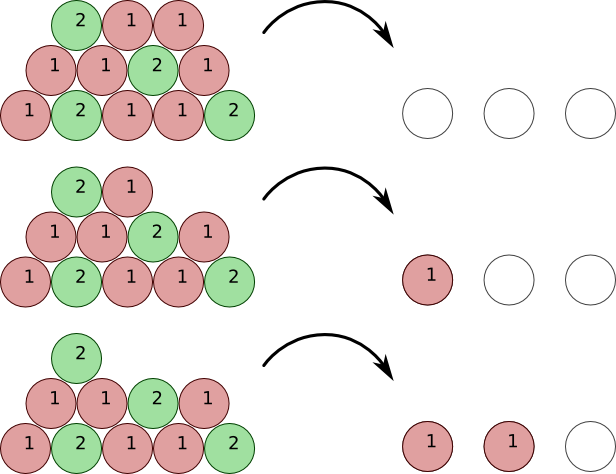
\includegraphics[height=7.11cm]{Figures/3Chapter/balls}
\end{psfrags}
\caption{Conditional probability can be employed to calculate the probability of multiple events occurring at the same time.}
\label{figure:Balls}
\end{center}
\end{figure}
\end{example}


\section{The Total Probability Theorem}

The probability of events $A$ and $B$ occurring at the same time can be calculated as a special case of \eqref{equation:SimultaneousEvents}.
For two events, this computational formula simplifies to
\begin{equation} \label{equation:ProbabilityIntersection}
\Pr (A \cap B) = \Pr (A|B) \Pr (B) .
\end{equation}
We can also obtain this equation directly from the definition of conditional probability.
This property is a key observation that plays a central role in establishing two important results, the \emph{total probability theorem} and \emph{Bayes' rule}.
To formulate these two theorems, we need to revisit the notion of a partition.
A collection of events $A_1, A_2, \ldots, A_n$ is said to be a \emph{partition} of the sample space $\Omega$ if these events are disjoint and their union is the entire sample space, \index{Partition}
\begin{equation*}
\bigcup_{k=1}^n A_k = \Omega .
\end{equation*}
Visually, a partition divides an entire set into disjoint subsets, as exemplified in Figure~\ref{figure:SetPartitiion2}.

\begin{figure}[htb]
\begin{center}
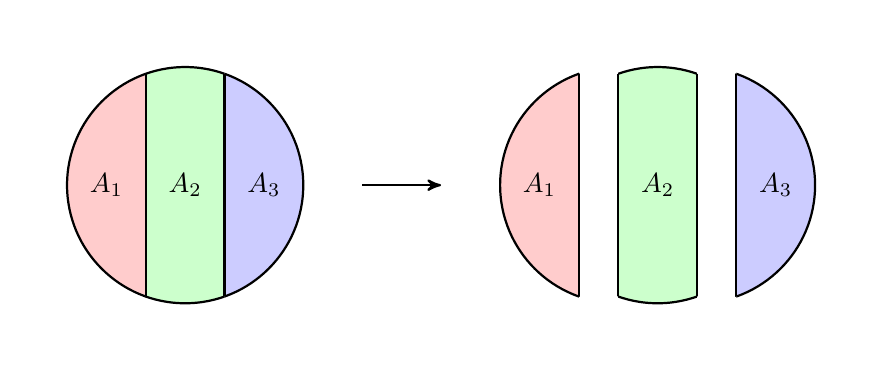
\begin{tikzpicture}
\begin{scope}
    \clip (-2cm,-2cm) rectangle (-0.5cm,2cm);
    \draw[thick,fill=red!20] (0,0) circle (1.5cm);
\end{scope}
\begin{scope}
    \clip (-0.5cm,-2cm) rectangle (0.5cm,2cm);
    \draw[thick,fill=green!20] (0,0) circle (1.5cm);
\end{scope}
\begin{scope}
    \clip (0.5cm,-2cm) rectangle (2cm,2cm);
    \draw[thick,fill=blue!20] (0,0) circle (1.5cm);
\end{scope}
\begin{scope}
    \clip (0,0) circle (1.5cm);
    \draw[thick] (-0.5cm,-2cm) rectangle (0.5cm,2cm);
\end{scope}
\coordinate [label=center:{$A_1$}] (A1b) at (-1cm,0);
\coordinate [label=center:{$A_2$}] (A2b) at (0cm,0);
\coordinate [label=center:{$A_3$}] (A3b) at (1cm,0);

\begin{scope}
    \clip (3.5cm,-2cm) rectangle (5cm,2cm);
    \draw[thick,fill=red!20] (5.5cm,0) circle (1.5cm);
\end{scope}
\begin{scope}
    \clip (5.5cm,0) circle (1.5cm);
    \draw[thick] (3.5cm,-2cm) rectangle (5cm,2cm);
\end{scope}
\begin{scope}
    \clip (5.5cm,-2cm) rectangle (6.5cm,2cm);
    \draw[thick,fill=green!20] (6cm,0) circle (1.5cm);
\end{scope}
\begin{scope}
    \clip (6cm,0) circle (1.5cm);
    \draw[thick] (5.5cm,-2cm) rectangle (6.5cm,2cm);
\end{scope}
\begin{scope}
    \clip (7cm,-2cm) rectangle (8.5cm,2cm);
    \draw[thick,fill=blue!20] (6.5cm,0) circle (1.5cm);
\end{scope}
\begin{scope}
    \clip (6.5cm,0) circle (1.5cm);
    \draw[thick] (7cm,-2cm) rectangle (8.5cm,2cm);
\end{scope}
\coordinate [label=center:{$A_1$}] (A1a) at (4.5cm,0);
\coordinate [label=center:{$A_2$}] (A2a) at (6cm,0);
\coordinate [label=center:{$A_3$}] (A3a) at (7.5cm,0);

\draw[->,thick,>=stealth'] (2.25cm,0) to (3.25cm,0);
\end{tikzpicture}
\caption{A partition of $\Omega$ can be formed by selecting a collection of subsets that are disjoint and whose union is $\Omega$.}
\label{figure:SetPartitiion2}
\end{center}
\end{figure}

\begin{theorem}[Total Probability Theorem] \label{theorem:TotalProbability} \index{Total probability theorem}
Let $A_1, A_2, \ldots, A_n$ be a collection of events that forms a partition of the sample space $\Omega$.
Suppose that $\Pr (A_k) > 0$ for all $k$.
Then, for any event $B$, we can write
\begin{equation*}
\begin{split}
\Pr (B) &= \Pr (A_1 \cap B) + \Pr (A_2 \cap B) + \cdots + \Pr (A_n \cap B) \\
&= \Pr (A_1) \Pr (B | A_1) + \Pr (A_2) \Pr (B | A_2) + \cdots + \Pr (A_n) \Pr (B | A_n ) .
\end{split}
\end{equation*}
\end{theorem}
\begin{proof}
The collection of events $A_1, A_2, \ldots, A_n$ forms a partition of the sample space $\Omega$.
We can therefore write
\begin{equation*}
B = B \cap \Omega = B \cap \left( \bigcup_{k=1}^n A_k \right) .
\end{equation*}
Since $A_1, A_2, \ldots, A_n$ are disjoint sets, the events $A_1 \cap B, A_2 \cap B, \ldots, A_n \cap B$ are also disjoint.
Combining these two facts, we get
\begin{equation*}
\begin{split}
\Pr (B)
&= \Pr \left( B \cap \left( \bigcup_{k=1}^n A_k \right) \right)
= \Pr \left( \bigcup_{k=1}^n (B \cap A_k) \right) \\
&= \sum_{k=1}^n \Pr \left( B \cap A_k \right)
= \sum_{k=1}^n \Pr (A_k) \Pr \left( B |A_k \right) ,
\end{split}
\end{equation*}
where the fourth equality follows from the third axiom of probability.
\end{proof}

\begin{figure}[htb]
\begin{center}
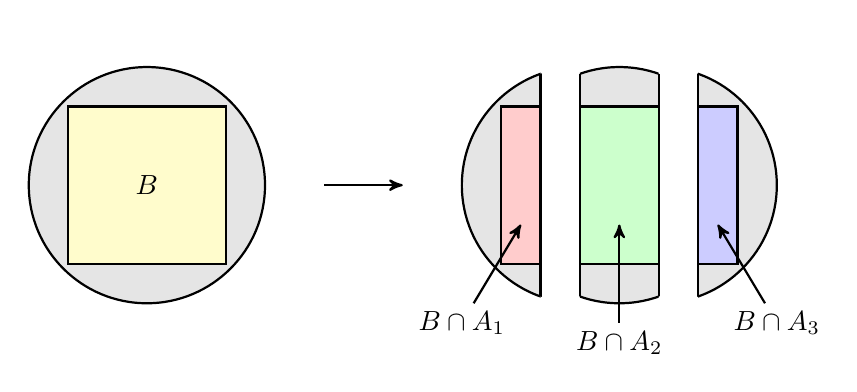
\begin{tikzpicture}
\draw[thick,fill=black!10] (0,0) circle (1.5cm);
\draw[thick,fill=yellow!20] (-1cm,-1cm) rectangle (1cm,1cm);
\coordinate [label=center:{$B$}] (B) at (0,0);

\begin{scope}
    \clip (3.5cm,-2cm) rectangle (5cm,2cm);
    \draw[thick,fill=black!10] (5.5cm,0) circle (1.5cm);
    \draw[thick,fill=red!20] (4.5cm,-1cm) rectangle (5.5cm,1cm);
\end{scope}
\begin{scope}
    \clip (5.5cm,0) circle (1.5cm);
    \draw[thick] (3.5cm,-2cm) rectangle (5cm,2cm);
\end{scope}
\begin{scope}
    \clip (5.5cm,-2cm) rectangle (6.5cm,2cm);
    \draw[thick,fill=black!10] (6cm,0) circle (1.5cm);
    \draw[thick,fill=green!20] (5cm,-1cm) rectangle (7cm,1cm);
\end{scope}
\begin{scope}
    \clip (6cm,0) circle (1.5cm);
    \draw[thick] (5.5cm,-2cm) rectangle (6.5cm,2cm);
\end{scope}
\begin{scope}
    \clip (7cm,-2cm) rectangle (8.5cm,2cm);
    \draw[thick,fill=black!10] (6.5cm,0) circle (1.5cm);
    \draw[thick,fill=blue!20] (5.5cm,-1cm) rectangle (7.5cm,1cm);
\end{scope}
\begin{scope}
    \clip (6.5cm,0) circle (1.5cm);
    \draw[thick] (7cm,-2cm) rectangle (8.5cm,2cm);
\end{scope}
\coordinate [label=center:{$B \cap A_1$}] (BA1) at (4cm,-1.75cm);
\draw[->,thick,>=stealth'] (4.15cm,-1.5cm) to (4.75cm,-0.5cm);
\coordinate [label=center:{$B \cap A_2$}] (BA2) at (6cm,-2cm);
\draw[->,thick,>=stealth'] (6cm,-1.75cm) to (6cm,-0.5cm);
\coordinate [label=center:{$B \cap A_3$}] (BA3) at (8cm,-1.75cm);
\draw[->,thick,>=stealth'] (7.85cm,-1.5cm) to (7.25cm,-0.5cm);

\draw[->,thick,>=stealth'] (2.25cm,0) to (3.25cm,0);
\end{tikzpicture}
\caption{The total probability theorem states that the probability of event $B$ can be computed by summing $\Pr(A_i \cap B)$ over all members of the partition $A_1, A_2, \ldots, A_n$.}
\label{figure:SetPartition3}
\end{center}
\end{figure}

A graphical interpretation of Theorem~\ref{theorem:TotalProbability} is illustrated in Figure~\ref{figure:SetPartition3}.
Event $B$ can be decomposed into the disjoint union of $A_1 \cap B, A_2 \cap B, \ldots, A_n \cap B$.
The probability of event $B$ can then be computed by adding the corresponding summands
\begin{equation*}
\Pr (A_1 \cap B), \Pr (A_2 \cap B), \ldots, \Pr (A_n \cap B) .
\end{equation*}

\begin{example}
An urn contains five green balls and three red balls.
A second urn contains three green balls and nine red balls.
One of the two urns is picked at random, with equal probabilities, and a ball is drawn from the selected urn.
We wish to compute the probability of obtaining a green ball.

In this problem, using a divide and conquer approach seems appropriate;
we therefore utilize the total probability theorem.
If the first urn is chosen, then the ensuing probability of getting a green ball is $5/8$.
One the other hand, if a ball is drawn from the second urn, the probability that it is green reduces to $3/12$.
Since the probability of selecting either urn is $1/2$, we can write the overall probability of getting a green ball as
\begin{equation*}
\begin{split}
\Pr (g) &= \Pr (g \cap U_1) + \Pr (g \cap U_2) \\
&= \Pr (g | U_1) \Pr (U_1) + \Pr (g | U_2) \Pr (U_2) \\
&= \frac{5}{8} \cdot \frac{1}{2} + \frac{3}{12} \cdot \frac{1}{2}
= \frac{7}{16}.
\end{split}
\end{equation*}
\end{example}


\section{Bayes' Rule}

The following result is also very useful.
It relates the conditional probability of $A$ given $B$ to the conditional probability of $B$ given $A$.

\begin{theorem}[Bayes' Rule] \index{Bayes' rule}
Let $A_1, A_2, \ldots, A_n$ be a collection of events that forms a partition of the sample space $\Omega$.
Suppose that $\Pr (A_k) > 0$ for all $k$.
Then, for any event $B$ such that $\Pr (B) > 0$, we can write
\begin{equation} \label{equation:BayesRule}
\begin{split}
\Pr (A_i | B)
&= \frac{ \Pr (A_i) \Pr (B | A_i) }{ \Pr (B) } \\
&= \frac{ \Pr (A_i) \Pr (B | A_i) }
{ \sum_{k=1}^n \Pr (A_k) \Pr (B | A_k) } .
\end{split}
\end{equation}
\end{theorem}
\begin{proof}
Bayes' rule is easily verified.
We expand the probability of $A_i \cap B$ using \eqref{equation:ProbabilityIntersection} twice, and we get
\begin{equation*}
\Pr (A_i \cap B) = \Pr (A_i | B) \Pr (B) = \Pr (B | A_i) \Pr (A_i).
\end{equation*}
Rearranging the terms yields the first equality.
The second equality in \eqref{equation:BayesRule} is obtained by applying Theorem~\ref{theorem:TotalProbability} to the denominator $\Pr(B)$.
\end{proof}

\begin{example}
April, a biochemist, designs a test for a latent disease.
If a subject has the disease, the probability that the test results turn out positive is $0.95$.
Similarly, if a subject does not have the disease, the probability that the test results come up negative is $0.95$.
Suppose that one percent of the population is infected by the disease.
We wish to find the probability that a person who tested positive has the disease.

Let $D$ denote the event that a person has the disease, and let $P$ be the event that the test results are positive.
Using Bayes' rule, we can compute the probability that a person who tested positive has the disease,
\begin{equation*}
\begin{split}
\Pr (D|P)
&= \frac{ \Pr(D) \Pr(P|D) }{ \Pr(D) \Pr(P|D) + \Pr(D^{\Complement}) \Pr(P|D^{\Complement}) } \\
&= \frac{ 0.01 \cdot 0.95 }{ 0.01 \cdot 0.95 + 0.99 \cdot 0.05 } \\
&\approx 0.1610 .
\end{split}
\end{equation*}
Although the test may initially appear fairly accurate, the probability that a person with a positive test carries the disease remains small.
\end{example}


\section{Independence}
\label{section:Independence}

Two events $A$ and $B$ are said to be \emph{independent} if $\Pr (A \cap B) = \Pr(A) \Pr(B)$. \index{Independence}
Interestingly, independence is closely linked to the concept of conditional probability.
If $\Pr(B) > 0$ and events $A$ and $B$ are independent, then
\begin{equation*}
\Pr (A | B) = \frac{ \Pr (A \cap B) }{\Pr (B)}
= \frac{ \Pr (A) \Pr(B) }{\Pr (B)}
= \Pr (A).
\end{equation*}
That is, the \emph{a priori} probability of event $A$ is identical to the \emph{a posteriori} probability of $A$ given $B$.
In other words, if $A$ is independent of $B$, then partial knowledge of $B$ contains no information about the likely occurrence of $A$.
We note that independence is a symmetric relation; if $A$ is independent of $B$, then $B$ is also independent of $A$.
It is therefore unambiguous to say that $A$ and $B$ are independent events.

\begin{example}
Suppose that two dice are rolled at the same time, a red die and a blue die.
We observe the numbers that appear on the upper faces of the two dice.
The sample space for this experiment is composed of thirty-six equally likely outcomes.
Consider the probability of getting a four on the red die given that the blue die shows a six,
\begin{equation*}
\begin{split}
\Pr (\{ r=4 \} | \{ b=6 \})
&= \frac{ \Pr (\{ r=4 \} \cap \{ b=6 \}) }
{ \Pr ( b=6 ) } \\
&= \frac{1}{6} = \Pr ( r=4 ) .
\end{split}
\end{equation*}
From this equation, we gather that
\begin{equation*}
\Pr (\{ r=4 \} \cap \{ b=6 \})
= \Pr ( r=4 ) \Pr ( b=6 ) .
\end{equation*}
As such, rolling a four on the red die and rolling a six on the blue die are independent events.

Similarly, consider the probability of obtaining a four on the red die given that the sum of the two dice is eleven,
\begin{equation*}
\begin{split}
\Pr (\{ r=4 \} | \{ r+b=11 \})
&= \frac{ \Pr (\{ r=4 \} \cap \{ r+b=11 \}) }
{ \Pr ( r+b=11 ) } = 0 \\
&\neq \frac{1}{6} = \Pr ( r=4 ) .
\end{split}
\end{equation*}
In this case, we conclude that getting a four on the red die and a sum total of eleven are not independent events.
\end{example}

The basic idea of independence seems intuitively clear: if knowledge about the occurrence of event $B$ has no impact on the probability of $A$, then these two events must be independent.
Yet, independent events are not necessarily easy to visualize in terms of their sample space.
A common mistake is to assume that two events are independent if they are disjoint.
Two mutually exclusive events can hardly be independent: if $\Pr (A) > 0$, $\Pr (B) > 0$, and $\Pr (A \cap B) = 0$ then
\begin{equation*}
\Pr (A \cap B) = 0 < \Pr (A) \Pr(B).
\end{equation*}
Hence, $A$ and $B$ cannot be independent if they are disjoint, non-trivial events.


\subsection{Independence of Multiple Events}

The concept of independence can be extended to multiple events.
The events $A_1, A_2, \ldots, A_n$ are \emph{independent} provided that \index{Independence}
\begin{equation} \label{equation:IndependenceMultipleEvents}
\Pr \left( \bigcap_{i \in \IndexSet} A_i \right)
= \prod_{i \in \IndexSet} \Pr (A_i) ,
\end{equation}
for every subset $\IndexSet$ of $\{1, 2, \ldots, n\}$.

For instance, consider a collection of three events, $A$, $B$ and $C$.
These events are independent whenever
\begin{equation} \label{equation:ThreeIndependentEvents}
\begin{split}
\Pr (A \cap B) &= \Pr (A) \Pr (B) \\
\Pr (A \cap C) &= \Pr (A) \Pr (C) \\
\Pr (B \cap C) &= \Pr (B) \Pr (C)
\end{split}
\end{equation}
and, in addition,
\begin{equation*}
\Pr (A \cap B \cap C) = \Pr (A) \Pr (B) \Pr(C) .
\end{equation*}
The three equalities in \eqref{equation:ThreeIndependentEvents} assert that $A$, $B$ and $C$ are \emph{pairwise independent}.
Note that the fourth equation does not follow from the first three conditions, nor does it imply any of them.
Pairwise independence does not necessarily imply independence.
This is illustrated below.

\begin{example}
A fair coin is flipped twice.
Let $A$ denote the event that heads is observed on the first toss.
Let $B$ be the event that heads is obtained on the second toss.
Finally, let $C$ be the event that the two coins show distinct sides.
These three events each have a probability of $1/2$.
Furthermore, we have
\begin{equation*}
\Pr (A \cap B) = \Pr (A \cap C) = \Pr (B \cap C) = \frac{1}{4}
\end{equation*}
and, therefore, these events are pairwise independent.
However, we can verify that
\begin{equation*}
\Pr (A \cap B \cap C) = 0 \neq \frac{1}{8} = \Pr (A) \Pr (B) \Pr (C) .
\end{equation*}
This shows that events $A$, $B$ and $C$ are not independent.
\end{example}

\begin{example}
Two dice are rolled at the same time, a red die and a blue die.
Let $A$ be the event that the number on the red die is odd.
Let $B$ be the event that the number on the red die is either two, three or four.
Also, let $C$ be the event that the product of the two dice is twelve.
The individual probabilities of these events are
\begin{align*}
\Pr (A) &= \Pr (r \in \{1, 3, 5\}) = \frac{1}{2} \\
\Pr (B) &= \Pr (r \in \{2, 3, 4\}) = \frac{1}{2} \\
\Pr (C) &= \Pr (r \times b = 12) = \frac{4}{36} .
\end{align*}
We note that these events are not pairwise independent because
\begin{align*}
\Pr (A \cap B) &= \frac{1}{6} \neq \frac{1}{4} = \Pr(A) \Pr(B) \\
\Pr (A \cap C) &= \frac{1}{36} \neq \frac{1}{18} = \Pr(A) \Pr(C) \\
\Pr (B \cap C) &= \frac{1}{12} \neq \frac{1}{18} = \Pr(B) \Pr(C) .
\end{align*}
Consequently, the multiple events $A$, $B$ and $C$ are not independent.
Still, the probability of these three events occurring simultaneously is
\begin{equation*}
\Pr (A \cap B \cap C) = \frac{1}{36}
= \frac{1}{2} \cdot \frac{1}{2} \cdot \frac{4}{36}
= \Pr (A) \Pr (B) \Pr (C) .
\end{equation*}
\end{example}

\subsection{Conditional Independence}

We introduced earlier the meaning of conditional probability, and we showed that the set of conditional probabilities $\{ \Pr (A|B) \}$ specifies a valid probability law.
It is therefore possible to discuss independence with respect to conditional probability.
We say that events $A_1$ and $A_2$ are \emph{conditionally independent}, given event $B$, if \index{Conditional independence}
\begin{equation*}
\Pr (A_1 \cap A_2 | B) = \Pr (A_1 | B) \Pr (A_2 | B) .
\end{equation*}
Note that if $A_1$ and $A_2$ are conditionally independent, we can use equation \eqref{equation:ConditionalProbability} to write
\begin{equation*}
\begin{split}
\Pr (A_1 \cap A_2 | B) &= \frac{ \Pr (A_1 \cap A_2 \cap  B) }{\Pr (B)} \\
&= \frac{ \Pr (B) \Pr (A_1 | B) \Pr (A_2 | A_1 \cap  B) }{\Pr (B)} \\
&= \Pr (A_1 | B) \Pr (A_2 | A_1 \cap  B) .
\end{split}
\end{equation*}
Under the assumption that $\Pr (A_1 | B) > 0$, we can combine the previous two expressions and get
\begin{equation*}
\Pr (A_2 | A_1 \cap  B) = \Pr (A_2 | B) .
\end{equation*}
This latter result asserts that, given event $B$ has taken place, the additional information that $A_1$ has also occurred does not affect the likelihood of $A_2$.
It is simple to show that conditional independence is a symmetric relation as well.

\begin{example}
Suppose that a fair coin is tossed until heads is observed.
The number of trials is recorded as the outcome of this experiment.
We denote by $B$ the event that the coin is tossed more than one time.
Moreover, we let $A_1$ be the event that the number of trials is an even number; and $A_2$, the event that the number of trials is less than six.
The conditional probabilities of $A_1$ and $A_2$, given that the coin is tossed more than once, are
\begin{align*}
\Pr (A_1 | B) &= \frac{ \Pr (A_1 \cap B) }{ \Pr (B) }
= \frac{1/3}{1/2} = \frac{2}{3} \\
\Pr (A_2 | B) &= \frac{ \Pr (A_2 \cap B) }{ \Pr (B) }
= \frac{15/32}{1/2} = \frac{15}{16} .
\end{align*}
The joint probability of events $A_1$ and $A_2$ given $B$ is equal to
\begin{equation*}
\begin{split}
\Pr (A_1 \cap A_2 | B) &= \frac{ \Pr (A_1 \cap A_2 \cap B) }{ \Pr (B) } \\
&= \frac{5/16}{1/2} = \frac{5}{8} = \frac{2}{3} \cdot \frac{15}{16} \\
&= \Pr (A_1 | B) \Pr (A_2 | B) .
\end{split}
\end{equation*}
We conclude that $A_1$ and $A_2$ are conditionally independent given $B$.
In particular, we have
\begin{align*}
\Pr (A_2 | A_1 \cap  B) &= \Pr (A_2 | B) \\
\Pr (A_1 | A_2 \cap  B) &= \Pr (A_1 | B) .
\end{align*}
We emphasize that events $A_1$ and $A_2$ are not independent with respect to the unconditional probability law.
\end{example}

Two events that are independent with respect to an unconditional probability law may not be conditionally independent.

\begin{example}
Two dice are rolled at the same time, a red die and a blue die.
We can easily compute the probability of simultaneously getting a two on the red die and a six on the blue die,
\begin{equation*}
\Pr (\{ r=2 \} \cap \{ b=6 \}) = \frac{1}{36}
= \Pr ( r=2 ) \Pr ( b=6 ) .
\end{equation*}
Clearly, these two events are independent.

Consider the probability of rolling a two on the red die and a six on the blue die given that the sum of the two dice is an odd number.
The individual conditional probabilities are given by
\begin{equation*}
\Pr (\{ r=2 \} | \{ r+b \text{ is odd} \})
= \Pr (\{ b=6 \} | \{ r+b \text{ is odd} \})
= \frac{1}{6},
\end{equation*}
whereas the joint conditional probability is
\begin{equation*}
\Pr (\{ r=2 \} \cap \{ b=6 \} | \{ r+b \text{ is odd} \})
= 0 .
\end{equation*}
These two events are not conditionally independent.
\end{example}

It is possible to extend the notion of conditional independence to several events.
The events $A_1, A_2, \ldots, A_n$ are conditionally independent given $B$ if
\begin{equation*}
\Pr \left( \bigcap_{i \in \IndexSet} A_i \Big| B \right)
= \prod_{i \in \IndexSet} \Pr (A_i | B)
\end{equation*}
for every subset $\IndexSet$ of $\{1, 2, \ldots, n\}$.
This definition is analogous to \eqref{equation:IndependenceMultipleEvents}, albeit using the appropriate conditional probability law.


\section{Equivalent Notations}

In the study of probability, we are frequently interested in the probability of multiple events occurring simultaneously.
So far, we have expressed the joint probability of events $A$ and $B$ using the notation $\Pr (A \cap B)$.
For mathematical convenience, we also represent the probability that two events occur at the same time by
\begin{equation*}
\Pr (A, B) = \Pr (A \cap B) .
\end{equation*}
This alternate notation easily extends to the joint probability of several events.
We denote the joint probability of events $A_1, A_2, \ldots, A_n$ by
\begin{equation*}
\Pr (A_1, A_2, \ldots, A_n) =
\Pr \left( \bigcap_{k=1}^n A_k \right) .
\end{equation*}
Conditional probabilities can be written using a similar format.
The probability of $A$ given events $B_1, B_2, \ldots, B_n$ becomes
\begin{equation*}
\Pr (A | B_1, B_2, \ldots, B_n) =
\Pr \left( A \bigg| \bigcap_{k=1}^n B_k \right) .
\end{equation*}
From this point forward, we use these equivalent notations interchangeably.


\section*{Further Reading}

\begin{small}
\begin{enumerate}
\item Ross, S., \emph{A First Course in Probability}, 7th edition, Pearson Prentice Hall, 2006: Chapter~3.
\item Bertsekas, D. P., and Tsitsiklis, J. N., \emph{Introduction to Probability}, Athena Scientific, 2002: Sections~1.3--1.5.
\item Miller, S. L., and Childers, D. G., \emph{Probability and Random Processes with Applications to Signal Processing and Communications}, 2004: Sections~2.4--2.6.
\item Gubner, J. A., \emph{Probability and Random Processes for Electrical and Computer Engineers}, Cambridge, 2006: Sections~1.5--1.6.
\end{enumerate}
\end{small}

 % No psfrags

%\setcounter{page}{47}
%\setcounter{chapter}{4}
%% \part{Discrete Random Variables}
\chapter{Discrete Random Variables}
\label{chapter:DiscreteRandomVariables}

Suppose that an experiment and a sample space are given.
A \emph{random variable} is a real-valued function of the outcome of the experiment. \index{Random variable}
In other words, the random variable assigns a specific number to every possible outcome of the experiment.
The numerical value of a particular outcome is simply called the \emph{value} of the random variable. \index{Value of a random variable}
Because of the structure of real numbers, it is possible to define pertinent statistical properties on random variables that otherwise do not apply to probability spaces in general.

\begin{figure}[ht]
\begin{center}
\begin{psfrags}
\psfrag{S}[l]{Sample Space}
\psfrag{1}[c]{$1$}
\psfrag{2}[c]{$2$}
\psfrag{3}[c]{$3$}
\psfrag{4}[c]{$4$}
\psfrag{5}[c]{$5$}
\psfrag{6}[c]{$6$}
\psfrag{7}[c]{$7$}
\psfrag{R}[r]{Real Numbers}
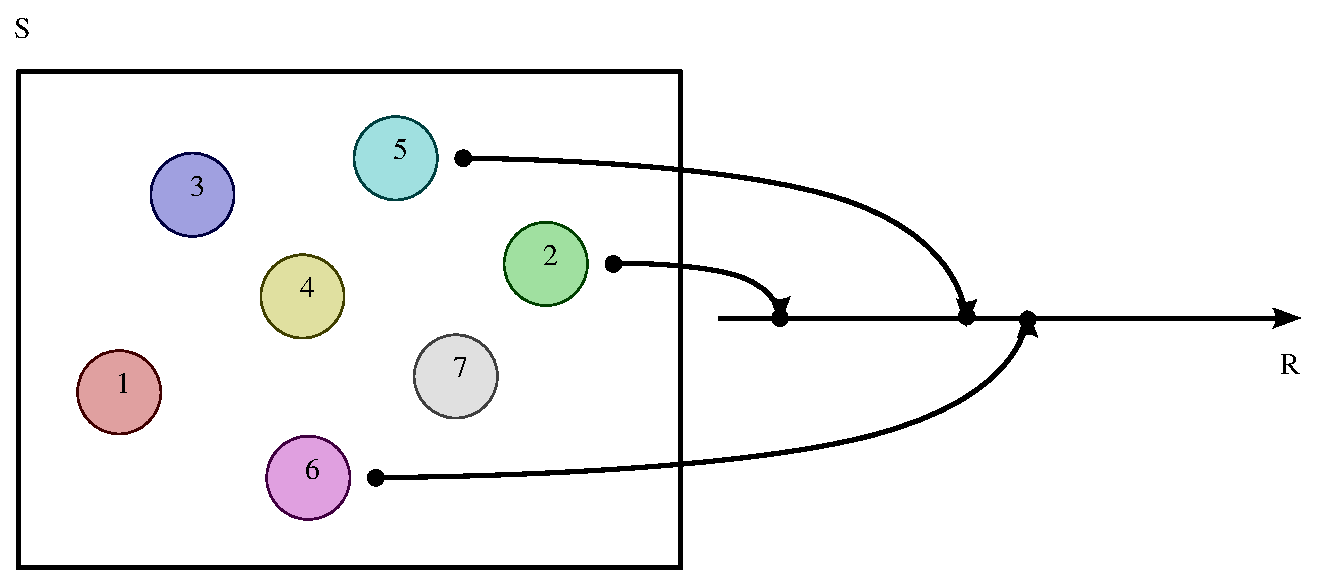
\includegraphics[height=4.96cm]{Figures/5Chapter/rv}
\caption{The sample space in this example has seven possible outcomes.
A random variable maps each of these outcomes to a real number.}
\end{psfrags}
\end{center}
\end{figure}

\begin{example}
There are six possible outcomes to the rolling of a fair die, namely each of the six faces.
These faces map naturally to the integers one through six.
The value of the random variable, in this case, is simply the number of dots that appear on the top face of the die.

\begin{figure}[ht]
\begin{center}
\begin{psfrags}
\psfrag{1}[c]{$1$}
\psfrag{2}[c]{$2$}
\psfrag{3}[c]{$3$}
\psfrag{4}[c]{$4$}
\psfrag{5}[c]{$5$}
\psfrag{6}[c]{$6$}
\includegraphics[height=5.99cm]{Figures/5chapter/rvdices}
\caption{This random variable takes its input from the rolling of a die and assigns to each outcome a real number that corresponds to the number of dots that appear on the top face of the die.}
\end{psfrags}
\end{center}
\end{figure}
\end{example}

The simplest class of random variables is the collection of \emph{discrete random variables}. \index{Discrete random variable}
A variable is called discrete if its range is finite or countably infinite; that is, if the random variable can only take a finite or countable number of values.

\begin{example}
Consider the experiment where a coin is tossed repetitively until heads is observed.
The corresponding function, which maps the number of tosses to an integer, is a discrete random variable that takes a countable number of values.
The range of this random variable is given by the positive integers $\{1, 2, \ldots \}$.
\end{example}

\section{Probability Mass Functions}

A discrete random variable $X$ is characterized by the probability of each of the elements in the range of $X$.
We identify the probabilities of individual elements in the range of $X$ using the \emph{probability mass function (PMF)} of $X$, which we denote by $p_X$. \index{Probability mass function (PMF)}
If $x$ is a possible value of $X$ then the \emph{probability mass} of $x$, written $p_X (x)$, is defined by
\begin{equation} \label{equation:PMF}
p_X (x) = \Pr ( \{ X = x \} ) = \Pr ( X = x ) .
\end{equation}
Equivalently, we can think of $p_X (x)$ as the probability of the set of all outcomes in $\Omega$ for which $X$ is equal to $x$,
\begin{equation*}
p_X (x)
= \Pr (  X^{-1} (x)  )
= \Pr ( \{ \omega \in \Omega | X(\omega) = x \} ) .
\end{equation*}

\begin{figure}[ht]
\begin{center}
\begin{psfrags}
\psfrag{S}[l]{Sample Space}
\psfrag{1}[c]{$1$}
\psfrag{2}[c]{$2$}
\psfrag{3}[c]{$3$}
\psfrag{4}[c]{$4$}
\psfrag{5}[c]{$5$}
\psfrag{6}[c]{$6$}
\psfrag{7}[c]{$7$}
\psfrag{x}[l]{$x$}
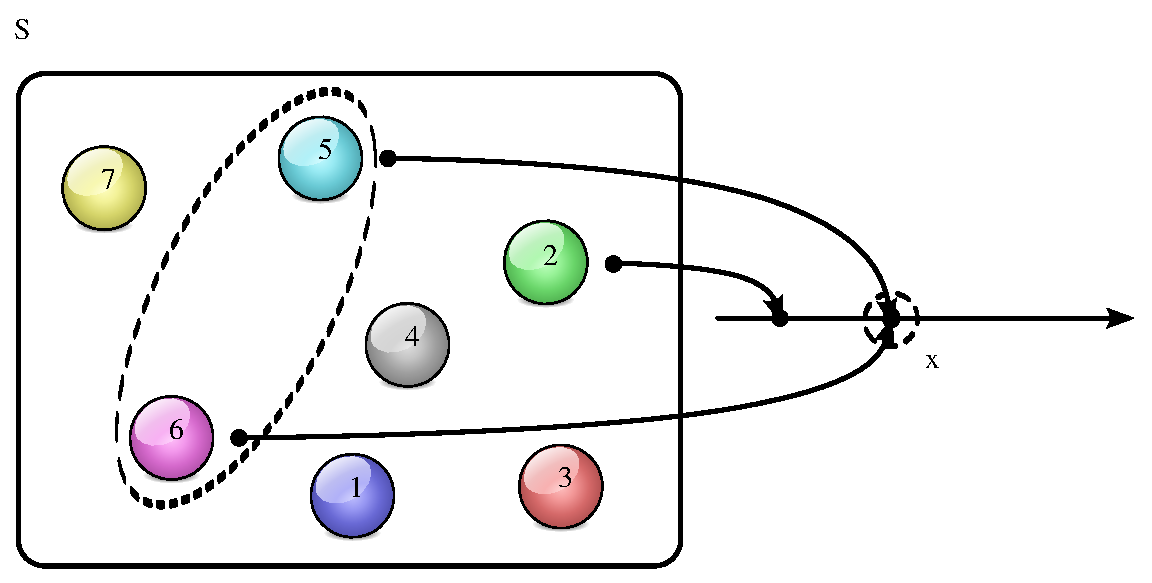
\includegraphics[height=4.97cm]{Figures/5Chapter/pmf}
\caption{The probability mass of $x$ is given by the probability of the set of all outcomes which $X$ maps to $x$.}
\end{psfrags}
\end{center}
\end{figure}


Let $X(\Omega)$ denote the collection of all the possible numerical values $X$ can take; this set is known as the range of $X$.
Using this notation, we can write
\begin{equation} \label{equation:NormalizationPMF}
\sum_{x \in X(\Omega)} p_X(x) = 1 .
\end{equation}
We emphasize that the sets defined by $\{ \omega \in \Omega | X(\omega) = x \}$ are disjoint and form a partition of the sample space $\Omega$, as $x$ ranges over all the possible values in $X (\Omega)$.
Thus, \eqref{equation:NormalizationPMF} follows immediately from the countable additivity axiom and the normalization axiom of probability laws.
In general, if $X$ is a discrete random variable and $S$ is a subset of $X(\Omega)$, we can write
\begin{equation} \label{equation:FunctionPMF}
\Pr (S) = \Pr \left( \{ \omega \in \Omega | X(\omega) \in S \} \right) = \sum_{x \in S} p_X (x) .
\end{equation}
This equation offers an explicit formula to compute the probability of any subset of $X (\Omega)$, provided that $X$ is discrete.

\begin{example}
An urn contains three balls numbered one, two and three.
Two balls are drawn from the urn without replacement.
We wish to find the probability that the sum of the two selected numbers is odd.

Let $\Omega$ be the set of ordered pairs corresponding to the possible outcomes of the experiment,
$\Omega = \{ (1, 2), (1, 3), (2, 1), (2, 3), (3, 1), (3, 2) \}$.
Note that these outcomes are equiprobable.
We employ $X$ to represent the sum of the two selected numbers.
The PMF of random variable $X$ is given by
\begin{equation*}
p_X (3) = p_X (4) = p_X (5) = \frac{1}{3}.
\end{equation*}
If $S$ denotes the event that the sum of the two numbers is odd, then the probability of the sum being odd can be computed as follows,
\begin{equation*}
\Pr (S) = \Pr ( \{ 3, 5 \} )
= p_X (3) + p_X (5) = \frac{2}{3} .
\end{equation*}
\end{example}


\section{Important Discrete Random Variables}

A number of discrete random variables appears frequently in problems related to probability.
These random variables arise in many different contexts, and they are worth getting acquainted with.
In general, discrete random variables occur primarily in situations where counting is involved.


\subsection{Bernoulli Random Variables}

The first and simplest discrete random variable is the \emph{Bernoulli random variable}. \index{Bernoulli random variable}
Let $X$ be a random variable that takes on only two possible numerical values, $X(\Omega) = \{0, 1\}$.
Then $X$ is a Bernoulli random variable and its PMF is given by
\begin{equation*}
p_X (x) = \left\{ \begin{array}{ll}
1 - p, & \text{if }x = 0 \\
p, & \text{if }x = 1
\end{array} \right.
\end{equation*}
where $p \in [0, 1]$.

\begin{figure}[ht]
\begin{center}
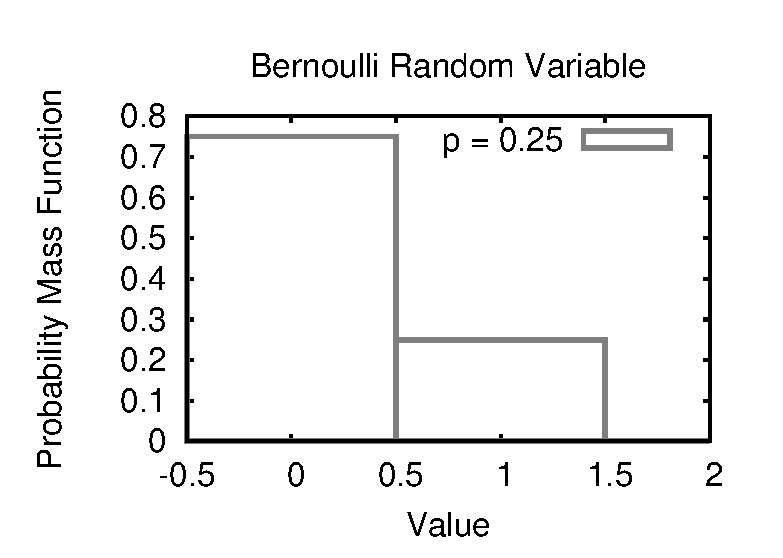
\includegraphics[width=8.5cm]{Figures/5chapter/bernoulli_pmf}
\end{center}
\caption{The PMF of a Bernoulli random variable appears above for parameter $p = 0.25$.}
\end{figure}

\begin{example}
Consider the flipping of a biased coin, for which heads is obtained with probability $p$ and tails is obtained with probability $1-p$.
A random variable that maps heads to one and tails to zero is a Bernoulli random variable with parameter~$p$.
In fact, every Bernoulli random variable is equivalent to the tossing of a coin.
\end{example}


\subsection{Binomial Random Variables}
\label{subsection:BinormialRandomVariables}

Multiple independent Bernoulli random variables can be combined to construct more sophisticated random variables.
Suppose $X$ is the sum of $n$ independent and identically distributed Bernoulli random variables.
Then $X$ is called a \emph{binomial random variable} with parameters $n$ and $p$. \index{Binomial random variable}
The PMF of $X$ is given by
\begin{equation*}
p_X (k) = \Pr (X = k)
= \binom{n}{k} p^k (1-p)^{n-k},
\end{equation*}
where $k = 0, 1, \ldots n$.
Note that we can easily verify that $X$ fulfills the normalization axiom,
\begin{equation*}
\sum_{k=0}^n \binom{n}{k} p^k (1-p)^{n-k}
= \left( p + (1-p) \right)^n = 1.
\end{equation*}

\begin{figure}[ht]
\begin{center}
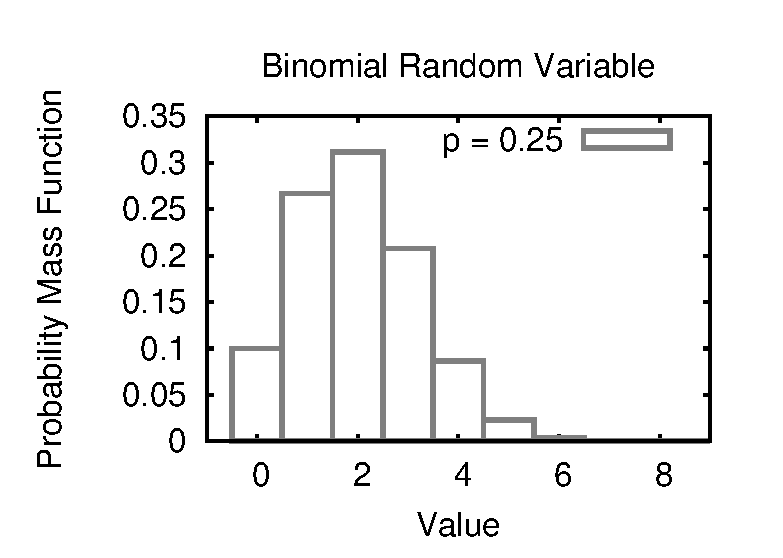
\includegraphics[width=8.5cm]{Figures/5chapter/binomial_pmf}
\end{center}
\caption{This figure shows a binomial random variable with parameters $n = 8$ and $p = 0.25$.}
\end{figure}

\begin{example} \label{BrazosSodaCompany1}
The Brazos Soda Company creates an ``Under the Caps'' promotion whereby a customer can win an instant cash prize of \$10 by looking under a bottle cap.
The likelihood to win is one in twelve, and it is independent from bottle to bottle.
A customer buys twelve bottles of soda from this company.
We wish to find the PMF of the number of winning bottles, which we denote by $X$.
Also, we want to compute the probability of winning more than \$40.

The random variable $X$ is binomial with parameters $n = 12$ and $p = 1/12$.
Its PMF is given by
\begin{equation*}
p_X (k) = \binom{12}{k} \left( \frac{1}{12} \right)^k
\left( \frac{11}{12} \right)^{n-k}
= \binom{12}{k} \frac{11^{n-k}}{12^n} ,
\end{equation*}
where $k = 0, 1, \ldots, 12$.
The probability of winning more than \$40 is
\begin{equation*}
\Pr (\$10 \times X > \$40)
= \Pr (X > 4)
= \sum_{k=5}^{12} \binom{12}{k} \frac{11^{n-k}}{12^n} .
\end{equation*}
\end{example}


\subsection{Poisson Random Variables}

The probability mass function of a \emph{Poisson random variable} is given by \index{Poisson random variable}
\begin{equation*}
p_X (k) = \frac{\lambda^k}{k!} e^{- \lambda}, \quad k = 0, 1, \ldots
\end{equation*}
where $\lambda$ is a positive number.
Note that, using Taylor series expansion,  we have
\begin{equation*}
\sum_{k = 0}^{\infty} p_X (k)
= \sum_{k = 0}^{\infty} \frac{\lambda^k}{k!} e^{- \lambda}
= e^{- \lambda} \sum_{k = 0}^{\infty} \frac{\lambda^k}{k!}
= e^{- \lambda} e^{\lambda} = 1 ,
\end{equation*}
which shows that this PMF fulfills the normalization axiom of probability laws.
The Poisson random variable is of fundamental importance when counting the number of occurrences of a phenomenon in a certain time period.
It finds extensive use in networking, inventory management and queueing applications.

\begin{figure}[ht]
\begin{center}
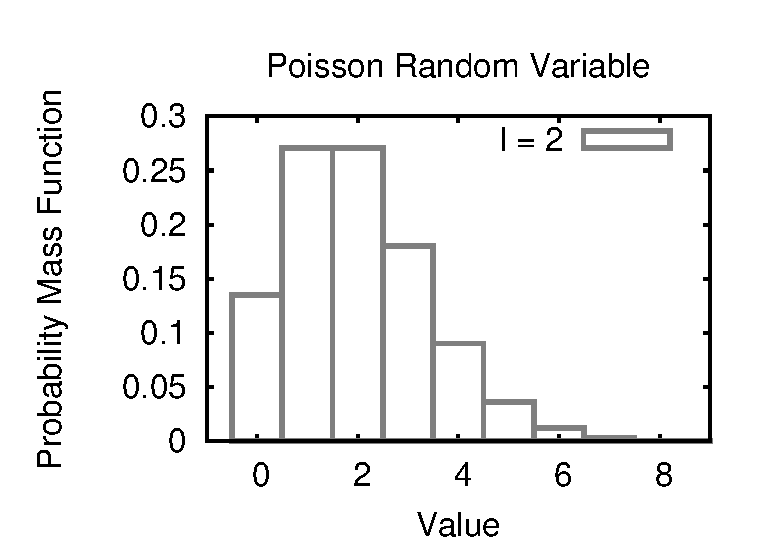
\includegraphics[width=8.5cm]{Figures/5chapter/poisson_pmf}
\caption{This figure shows the PMF of a Poisson random variable with parameter $\lambda = 2$.  Note that the values of the PMF are only present for $k = 0, 1, \ldots, 8$.}
\end{center}
\end{figure}

\begin{example}
Requests at an Internet server arrive at a rate of $\lambda$ connections per second.
The number of service requests per second is modeled as a random variable with a Poisson distribution.
We wish to find the probability that no service requests arrive during a time interval of one second.

Let $N$ be a random variable that represents the number of requests that arrives within a span of one second.
By assumption, $N$ is a Poisson random variable with PMF
\begin{equation*}
p_N (k) = \frac{ \lambda^k }{k!} e^{-\lambda} .
\end{equation*}
The probability that no service requests arrive in one second is simply given by $p_N (0) = e^{-\lambda}$.
\end{example}

It is possible to obtain a Poisson random variable as the limit of a sequence of binomial random variables.
Fix $\lambda$ and let $p_n = \lambda/n$.
For $k = 1, 2, \ldots n$, we define the PMF of the random variable $X_n$ as
\begin{equation*}
\begin{split}
p_{X_n} (k) &= \Pr (X_n = k)
= \binom{n}{k} p_n^k (1-p_n)^{n-k} \\
&= \frac{n!}{k!(n-k)!} \left( \frac{\lambda}{n} \right)^k
\left( 1 - \frac{\lambda}{n} \right)^{n-k} \\
&= \frac{n!}{n^k (n-k)!} \frac{\lambda^k}{k!}
\left( 1 - \frac{\lambda}{n} \right)^{n-k} .
\end{split}
\end{equation*}
In the limit, as $n$ approaches infinity, we get
\begin{equation*}
\lim_{n \rightarrow \infty} p_{X_n} (k)
= \lim_{n \rightarrow \infty} \frac{n!}{n^k (n-k)!} \frac{\lambda^k}{k!}
\left( 1 - \frac{\lambda}{n} \right)^{n-k}
= \frac{\lambda^k}{k!} e^{- \lambda} .
\end{equation*}
Thus, the sequence of binomial random variables $\{ X_n \}$ converges in distribution to the Poisson random variable $X$.

\begin{figure}[ht]
\begin{center}
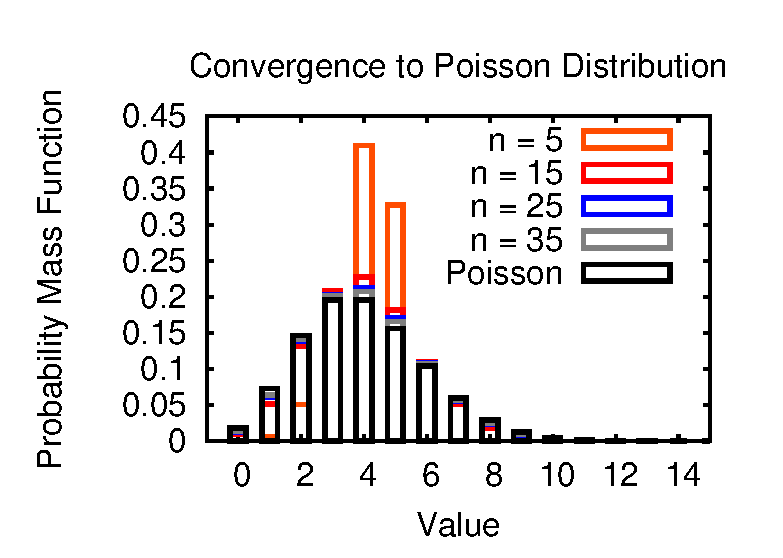
\includegraphics[width=8.5cm]{Figures/5chapter/convergence_pmf}
\end{center}
\caption{The levels of a binomial PMF with parameter $p = \lambda/n$ converge to the probabilities of a Poisson PMF with parameter $\lambda$ as $n$ increases to infinity.}
\end{figure}

This discussion suggests that the Poisson PMF can be employed to approximate the PMF of a binomial random variable in certain circumstances.
Suppose that $Y$ is a binomial random variable with parameters $n$ and $p$.
If $n$ is large and $p$ is small then the probability that $Y$ equals $k$ can be approximated by
\begin{equation*}
p_{Y} (k) = \frac{n!}{n^k (n-k)!} \frac{\lambda^k}{k!}
\left( 1 - \frac{\lambda}{n} \right)^{n-k}
\approx \frac{\lambda^k}{k!} e^{- \lambda} ,
\end{equation*}
where $\lambda = n p$.
The latter expression can be computed numerically in a straightforward manner.

\begin{example}
The probability of a bit error on a wireless communication channel is equal to $10^{-2}$.
We wish to approximate the probability that a block of $1000$ bits has four or more errors.

Assume that the probability of individual errors is independent from bit to bit.
The transmission of each bit can be modeled as a Bernoulli trial, with a zero indicating a correct transmission and a one representing a bit error.
The total number of bit errors in $1000$ transmissions then corresponds to a binomial random variable with parameters $n = 1000$ and $p = 10^{-2}$.
The probability of making four or more errors can be approximated using a Poisson random variable with constant $\lambda = np = 10$.
Thus, we can approximate the probability that a block of $1000$ bits has four or more errors by
\begin{equation*}
\begin{split}
\Pr [ N \geq 4 ] &= 1 - \Pr [ N < 4 ]
\approx 1 - \sum_{k=0}^3 \frac{\lambda^k}{k!} e^{-\lambda} \\
&= 1 - e^{-10} \left( 1 + 10 + 50 + \frac{500}{3} \right) \\
&\approx 0.01034 .
\end{split}
\end{equation*}
% The exact value in this case is
\end{example}


\subsection{Geometric Random Variables}

Consider a random experiment where a Bernoulli trial is repeated multiple times until a one is observed.
At each time step, the probability of getting a one is equal to $p$ and the probability of getting a zero is $1-p$.
The number of trials carried out before completion, which we denote by $X$, is recorded as the outcome of the experiment.
The random variable $X$ is a \emph{geometric random variable}, and its PMF is given by \index{Geometric random variable}
\begin{equation*}
p_X (k) = (1-p)^{k-1} p, \quad k = 1, 2, \ldots
\end{equation*}
We stress that $(1-p)^{k-1} p$ simply represents the probability of obtaining a sequence of $k-1$ zero immediately followed by a one.

\begin{figure}[ht]
\begin{center}
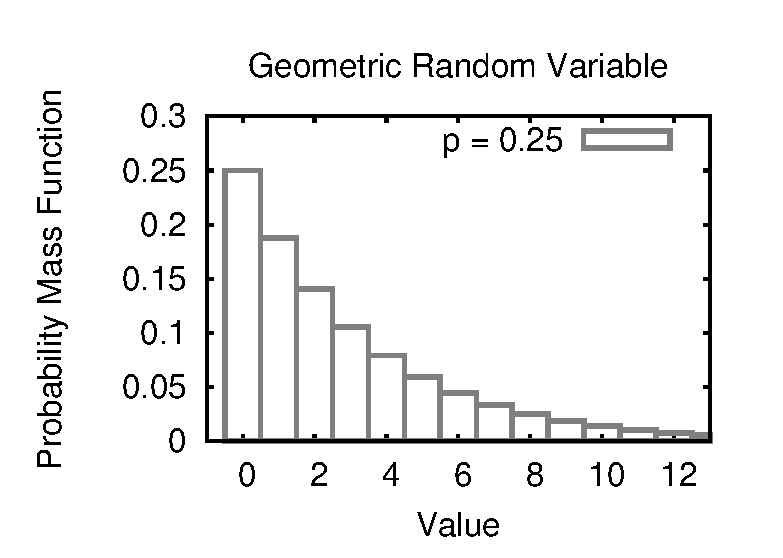
\includegraphics[width=8.5cm]{Figures/5chapter/geometric_pmf}
\end{center}
\caption{The PMF of a geometric random variable is a decreasing function of $k$.
It is plotted above for $p = 0.25$.
The values of the PMF are only present for $k = 1, 2, \ldots, 12$.}
\end{figure}

\begin{example}
The Brazos Soda Company introduces another ``Under the Caps'' promotion.
This time, a customer can win an additional bottle of soda by looking under the cap of her bottle.
The probability to win is $1/5$, and it is independent from bottle to bottle.
A customer purchases one bottle of soda from the Brazos Soda company and hence enters the contest.
For every extra bottle of soda won by looking under the cap, the customer gets an additional chance to play.
We wish to find the PMF of the number of bottles obtained by this customer.

Let $X$ denote the total number of bottles obtained by this customer.
The random variable $X$ is geometric and its PMF is
\begin{equation*}
p_X (k) = \left( \frac{1}{5} \right)^{k-1} \frac{4}{5},
\end{equation*}
where $k = 1, 2, \ldots$
\end{example}

\paragraph{Memoryless Property:}
A remarkable aspect of the geometric random variable is that it satisfies the \emph{memoryless property}, \index{Memoryless property}
\begin{equation*}
\Pr (X = k + j | X > k) = \Pr (X = j).
\end{equation*}
This can be established using the definition of conditional probability.
Let $X$ be a geometric random variable with parameter $p$, and assume that $k$ and $j$ are positive integers.
We can write the conditional probability of $X$ as
\begin{equation*}
\begin{split}
\Pr (X = k + j | X > k)
&= \frac{\Pr( \{ X =  k + j \} \cap \{ X > k \} ) }{ \Pr ( X > k ) } \\
&= \frac{\Pr( X = k + j ) }{ \Pr ( X > k ) }
= \frac{(1 - p)^{k + j - 1} p }{ (1 - p)^k  } \\
&= (1 - p)^{j - 1} p
= \Pr (X = j).
\end{split}
\end{equation*}
In words, the probability that the number of trials carried out before completion is $k + j$, given $k$ unsuccessful trials, is equal to the unconditioned probability that the total number of trials is $j$.
It can be shown that the geometric random variable is the only discrete random variable that possesses the memoryless property.


\subsection{Discrete Uniform Random Variables}

A finite random variable where all the possible outcomes are equally likely is called a \emph{discrete uniform random variable}. \index{Uniform random variable (discrete)}
Let $X$ be a uniform random variable taking value in $X (\Omega) = \{ 1, 2, \ldots, n \}$.
Its PMF is therefore given by
\begin{equation*}
p_X (k) = \left\{ \begin{array}{ll}
1/n, & \text{if }k = 1, 2, \ldots, n \\
0, & \text{otherwise} .
\end{array} \right.
\end{equation*}
We encountered specific cases of this random variable before.
The tossing of a fair coin and the rolling of a die can both be used to construct uniform random variables.

\begin{figure}[ht]
\begin{center}
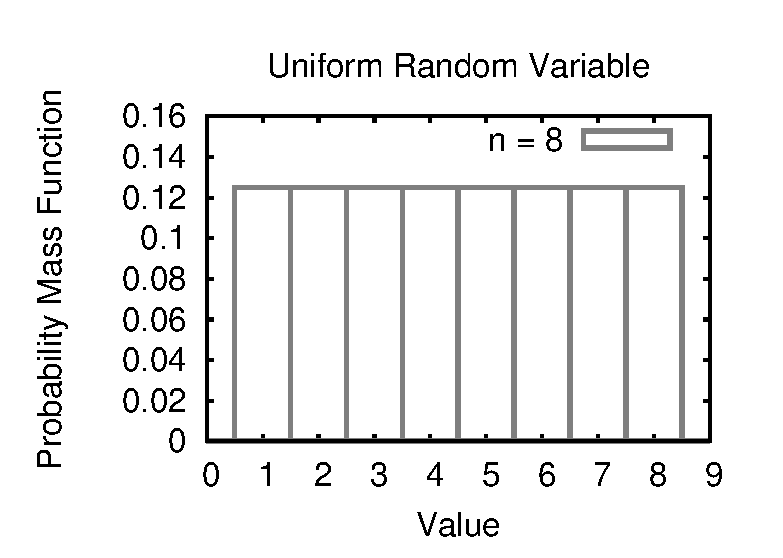
\includegraphics[width=8.5cm]{Figures/5chapter/uniform_pmf}
\end{center}
\caption{A uniform random variable corresponds to a situation where all the possible values of the random variable are equally likely.
It is shown above for the case where $n = 8$.}
\end{figure}


\section{Functions of Random Variables}
\label{subsection:FunctionDiscreteRV}
\index{Functions of Random Variables}

Recall that a random variable is a function of the outcome of an experiment.
Given a random variable $X$, it is possible to create a new random variable $Y$ by applying a real-valued function $g(\cdot)$ to $X$.
If $X$ is a random variable then $Y = g(X)$ is also a random variable since it associates a numerical value to every outcome of the experiment.
In particular, if $\omega \in \Omega$ is the outcome of the experiment, then $X$ takes on value $x = X(\omega)$ and $Y$ takes on value $Y(\omega) = g(x)$.

\begin{figure}[htb!]
\begin{center}
\begin{psfrags}
\psfrag{1}[c]{$1$}
\psfrag{2}[c]{$2$}
\psfrag{3}[c]{$3$}
\psfrag{4}[c]{$4$}
\psfrag{5}[c]{$5$}
\psfrag{S}[l]{Sample Space}
\psfrag{X}[c]{$X$}
\psfrag{Y}[c]{$Y = g(X)$}
\includegraphics[height=4.97cm]{Figures/5Chapter/fcn}
\end{psfrags}
\caption{A real-valued function of a random variable is a random variable itself.
In this figure, $Y$ is obtained by passing random variable $X$ through a function $g$.}
\end{center}
\end{figure}

Furthermore, if $X$ is a discrete random variable, then so is $Y$.
The set of all the possible values $Y$ can take is denoted by $g(X(\Omega))$, and the number of elements in $g(X(\Omega))$ is no greater than the number of elements in $X(\Omega)$.
The PMF of $Y$, which we represent by $p_Y (y)$, is obtained as follows.
If $y \in g(X(\Omega))$ then
\begin{equation} \label{equation:DefinitionFunctionPMF}
p_Y (y) = \sum_{ \{x \in X(\Omega) | g(x) = y \} } p_X (x) ;
\end{equation}
otherwise, $p_Y (y) = 0$.
In particular, $p_Y (y)$ is non-zero only if there exists an $x \in X(\Omega)$ such that $g(x) = y$ and $p_X (x) > 0$.

\begin{example}
Let $X$ be a random variable and let $Y = g(X) = aX + b$, where $a$ and $b$ are constant.
That is, $Y$ is an affine function of $X$.
Suppose that $a \neq 0$, then the probability of $Y$ being equal to value $y$ is given by
\begin{equation*}
p_Y(y) = p_X \left( \frac{ y - b }{a} \right) .
\end{equation*}
\end{example}

Linear and affine functions of random variables are commonplace in probability.
In Example~\ref{BrazosSodaCompany1}, for instance, we have implicitly used the linear function $Y = 10 X$ to compute the probability of winning more than \$40.


\section*{Further Reading}

\begin{small}
\begin{enumerate}
\item Ross, S., \emph{A First Course in Probability}, 7th edition, Pearson Prentice Hall,2006: Sections~4.1--4.2, 4.6--4.8.
\item Bertsekas, D.P., and Tsitsiklis, J.N., \emph{Introduction to Probability}, Athena Scientific, 2002: Sections~2.1--2.3.
\end{enumerate}
\end{small}


%\chapter{Expectations (Discrete)}
\label{chapter:ExpectationsDiscrete}

When a large collection of data is gathered, one is typically interested not necessarily in each individual data point, but rather in certain descriptive quantities such as the average or the median.
The same is true for random variables.
The PMF of random variable $X$ provides a complete characterization of the distribution of $X$ by specifying the probability of every possible value of $X$.
Still, it may be desirable to summarize the information contained in the PMF of a random variable into a few parameters.
One way to achieve this goal and obtain meaningful descriptive quantities is through the concept of expectation.


\section{Expected Value}

The \emph{expected value} $\Expect [X]$ of random variable $X$ is defined by \index{Expected value}
\begin{equation} \label{equation:DiscreteMean}
\Expect [X] = \sum_{x \in X(\Omega)} x p_X (x) ,
\end{equation}
provided that the sum converges absolutely.
If the above sum is not absolutely convergent, then $X$ is said not to possess an expected value.
In some sense, the expected value $\Expect [X]$ offers useful information about the underlying random variable $X$ without giving a comprehensive and overly detailed description.
The expected value of a random variable, as defined in \eqref{equation:DiscreteMean}, is also called the \emph{mean} of $X$. \index{Mean}
It is important to realize that $\Expect [X]$ is not a function of random variable $X$; rather, it is a function of the PMF of $X$.

\begin{example}
A fair die is rolled once, with the number of dots appearing on the top face taken as the value of the corresponding random variable.
The expected value of the roll can be computed as
\begin{equation*}
\sum_{k=1}^6 \frac{k}{6} = \frac{42}{12} = 3.5 .
\end{equation*}
Thus, the mean of this random variable is $3.5$.
\end{example}

\begin{example}
Assume that a standard coin is flipped repetitively until heads is observed.
The total number of tosses performed during this experiment is assigned as the value of random variable $X$.
The possible values that $X$ can take are therefore given by $X (\Omega) = \{ 1, 2, \ldots \}$.
Recall that the PMF of $X$ is equal to $p_X(k) = 2^{-k}$, where $k$ is a positive integer.
The expected value of this geometric random variable can be computed as
\begin{equation*}
\Expect [X] = \sum_{k=1}^{\infty} \frac{k}{2^k}
= 2.
\end{equation*}
In other words, the expected number of tosses until the coin lands on heads is two.
\end{example}

In both cases, computing the expected value of the random variable provides a concise summary of its behavior.
This procedure takes as input the PMF, a detailed characterization of the random variable, and returns a much simplified and yet relevant scalar attribute, its mean.


\section{Functions and Expectations}

The mean offers only one instance where the distribution of a random variable is condensed into a scalar quantity.
The notion of \emph{expectation} can be combined with traditional functions to create alternate descriptions and other meaningful attributes. \index{Expectation}

Suppose that $X$ is a discrete random variable.
Let $g: X(\Omega) \mapsto \mathbb{R}$ be a real-valued function on the range of $X$, and consider the expectation of $g(X)$.
One way to determine the expected value of $g(X)$ is to first notice that $Y = g(X)$ is itself a random variable, find the PMF of $Y$, and then apply the definition of expected value provided in \eqref{equation:DiscreteMean}.

Yet, there is another and more direct way to compute this quantity.
The \emph{expectation} of $g(X)$ can be written as \index{Expectation}
\begin{equation} \label{equation:DiscreteExpectation}
\Expect \left[ g(X) \right]
= \sum_{x \in X(\Omega)} g(x) p_X (x) .
\end{equation}
Again, it is worth mentioning that there exist random variables and functions for which the above sum does not converge.
In such cases, we simply say that the expected value of $g(X)$ does not exist.
Also, we note that the mean $\Expect [X]$ is a special case of \eqref{equation:DiscreteExpectation} where $g(X) = X$.
We explore additional examples below.

\begin{example}
The simplest possible scenario for \eqref{equation:DiscreteExpectation} is a situation where the function $g(x)$ is a constant.
In this case, the expectation of $g(X) = c$ is equal to
\begin{equation*}
\Expect [ c ]
= \sum_{x \in X(\Omega)} c p_X (x)
= c \sum_{x \in X(\Omega)} p_X (x)
= c,
\end{equation*}
where the last inequality follows from the normalization axiom of probability laws.
The expectation of a constant is always the constant itself.
\end{example}

\begin{example}
Let $S$ be a subset of the real numbers, and define the \emph{indicator function} of $S$ by \index{Indicator function}
\begin{equation*}
\IndicatorFcn_S (x) = \begin{cases} 1, & x \in S\\
0, & x \notin S . \end{cases}
\end{equation*}
The expectation of $\IndicatorFcn_S (x)$ is equal to
\begin{equation*}
\Expect \left[ \IndicatorFcn_S (x) \right]
= \sum_{x \in X(\Omega)} \IndicatorFcn_S (x) p_X(x)
= \sum_{x \in S} p_X(x)
= \Pr (x \in S) .
\end{equation*}
That is, the expectation of the indicator function of $S$ is simply the probability that $X$ takes on value in $S$.
\end{example}

Let random variable $Y$ be defined by applying real-valued function $g(\cdot)$ to $X$, with $Y = g(X)$.
The mean of $Y$ is equal to the expectation of $g(X)$, and we know from our previous discussion that this value can be obtained by applying two different formulas.
For consistency, we need to make sure that we get a same solution using either approach.

First, we can apply \eqref{equation:DiscreteMean} directly to $Y$, and obtain
\begin{equation*}
\Expect [Y] = \sum_{y \in g(X(\Omega))} y p_Y(y),
\end{equation*}
where $p_Y (\cdot)$ is the PMF of $Y$ provided by \eqref{equation:FunctionPMF}.
Alternatively, using \eqref{equation:DiscreteExpectation}, we have
\begin{equation*}
\Expect [Y] = \Expect [g(X)] = \sum_{x \in X(\Omega)} g(x) p_X(x) .
\end{equation*}
We can verify that these two procedures lead to a same solution as follows.
Recall that the PMF of $Y$ evaluated at $y$ is obtained by summing the values of $p_X(\cdot)$ over all $x \in X(\Omega)$ such that $g(x) = y$.
Mathematically, this can be expressed as $p_Y (y) = \sum_{ \{x \in X(\Omega) | g(x) = y \} } p_X (x)$.
Using this result, we get
\begin{equation*}
\begin{split}
\Expect [Y] &= \sum_{y \in g(X(\Omega))} y p_Y(y)
= \sum_{y \in g(X(\Omega))} y
\sum_{\{x \in X(\Omega) | g(x) = y\}} p_X(x) \\
&= \sum_{y \in g(X(\Omega))}
\sum_{\{x \in X(\Omega) | g(x) = y\}} y p_X(x) \\
&= \sum_{y \in g(X(\Omega))}
\sum_{\{x \in X(\Omega) | g(x) = y\}} g(x) p_X(x) \\
&= \sum_{x \in X(\Omega)} g(x) p_X(x)
= \Expect [g(X)] .
\end{split}
\end{equation*}
We emphasize that summing over all possible values of $Y$ and after summing over the preimage of $y$ for every $y \in Y(\Omega)$ is equivalent to summing over all $x \in X(\Omega)$.
Thus, we have shown that computing the expectation of a function using the two methods outlined above leads to a same solution.

\begin{example}
Brazos Extreme Events Radio creates the ``Extreme Trio'' contest.
To participate, a person must fill out an application card.
Three cards are drawn from the lot and each winner is awarded \$1,000.
While a same participant can send multiple cards, he or she can only win one grand prize.
At the time of the drawing, the radio station has accumulated a total of 100 cards.
David, an over-enthusiastic listener, is accountable for half of these cards.
We wish to compute the amount of money David expects to win under this promotion.

Let $X$ be the number of cards drawn by the radio station written by David.
The PMF of $X$ is given by
\begin{equation*}
p_X(k) = \frac{\binom{50}{k} \binom{50}{3-k}}{\binom{100}{3}}
\quad k \in \{ 0, 1, 2, 3 \}.
\end{equation*}
The money earned by David can be expressed as $g(k) = 1000 \min \{ k,1 \}$.
It follows that the expected amount of money he receives is equal to
\begin{equation*}
\sum_{k=0}^3 \left( 1000 \min \{ k, 1 \} \right) p_X(k)
= 1000 \cdot \frac{29}{33} .
\end{equation*}
Alternatively, we can define $Y = 1000 \min \{ X, 1 \}$.
Clearly, $Y$ can only take on one of two possible values, $0$ or $1000$.
Evaluating the PMF of $Y$, we get $p_Y(0) = p_X(0) = 4/33$ and $p_Y(1000) = 1 - p_Y(0) = 29/33$.
The expected value of $Y$ is equal to
\begin{equation*}
0 \cdot p_Y(0) + 1000 \cdot p_Y(1000) = 1000 \cdot \frac{29}{33} .
\end{equation*}
As anticipated, both methods lead to the same answer.
The expected amount of money won by David is roughly \$878.79.
\end{example}


\subsection{The Mean}

As seen at the beginning of this chapter, the simplest non-trivial expectation is the \emph{mean}.  \index{Mean}
We provide two additional examples for the mean, and explore a physical interpretation of its definition below.

\begin{example}
Let $X$ be a geometric random variable with parameter $p$ and PMF
\begin{equation*}
p_X (k) = (1-p)^{k-1} p, \quad k = 1, 2, \ldots
\end{equation*}
The mean of this random variable is
\begin{equation*}
\begin{split}
\Expect [X] &= \sum_{k=1}^{\infty} k (1-p)^{k-1} p
= p \sum_{k=1}^{\infty} k (1-p)^{k-1}
= \frac{1}{p} .
\end{split}
\end{equation*}
\end{example}

\begin{example}
Let $X$ be a binomial random variable with parameters $n$ and $p$.
The PMF of $X$ is given by
\begin{equation*}
p_X (k) = \binom{n}{k} p^k (1-p)^{n-k}, \quad k = 0, 1, \ldots, n.
\end{equation*}
The mean of this binomial random variable can therefore be computed as
\begin{equation*}
\begin{split}
\Expect [X] &= \sum_{k=0}^n k \binom{n}{k} p^k (1-p)^{n-k} \\
&= \sum_{k=1}^n \frac{n!}{(k-1)!(n-k)!} p^k (1-p)^{n-k} \\
&= \sum_{\ell=0}^{n-1} \frac{n!}{\ell!(n-1-\ell)!} p^{\ell+1} (1-p)^{n-\ell-1} \\
&= n p \sum_{\ell=0}^{n-1} \binom{n-1}{\ell} p^{\ell} (1-p)^{n-1-\ell} \\
&= n p .
\end{split}
\end{equation*}
Notice how we rearranged the sum into a familiar form to compute its value.
\end{example}

It may be insightful to relate the mean of a random variable to classical mechanics.
Let $X$ be a random variable and suppose that, for every $x \in X(\Omega)$, we place a pebble of mass $p_X(x)$ at position $x$ along a real line.
The mean of random variable $X$ as defined in \eqref{equation:DiscreteMean} coincides with the center of mass of the particles.

\begin{example}
Let $X$ be a Bernoulli random variable such that
\begin{equation*}
p_X (x) = \left\{ \begin{array}{ll}
0.25, & \text{if }x = 0 \\
0.75, & \text{if }x = 1.
\end{array} \right.
\end{equation*}
The mean of $X$ is given by
\begin{equation*}
\Expect [X] = 0 \times 0.25 + 1 \times 0.75 = 0.75 .
\end{equation*}
Consider a two-particle system with masses $m_1 = 0.25$ and $m_2 = 0.75$, respectively.
In the coordinate system illustrated below, the particles are located at positions $x_1 = 0$ and $x_2 = 1$.
From classical mechanics, we know that their center of mass can be expressed as
\begin{equation*}
\frac{ m_1 x_1 + m_2 x_2 }{ m_1 + m_2 } = 0.75 .
\end{equation*}
The center of mass thus corresponds to the mean of $X$.

\begin{figure}[ht]
\begin{center}
\begin{psfrags}
\psfrag{x1}[c]{$x_1$}
\psfrag{x2}[c]{$x_2$}
\psfrag{c}[c]{Center of Mass}
\psfrag{r}[c]{$\mathbb{R}$}
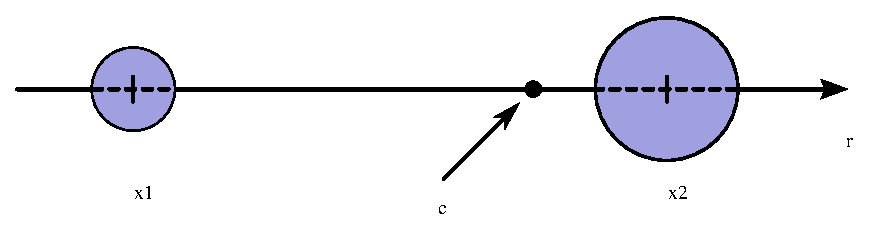
\includegraphics[height=1.8cm]{Figures/6Chapter/mass}
\end{psfrags}
\end{center}
\caption{The center of mass on the figure is indicated by the tip of the arrow.}
\end{figure}
\end{example}


\subsection{The Variance}

A second common descriptive quantity associated with random variable $X$ is its \emph{variance}, which we denote by $\Var [X]$. \index{Variance}
It is defined by
\begin{equation} \label{equation:VarianceExplicit}
\Var [X] = \Expect \left[ \left( X - \Expect [X] \right)^2 \right] .
\end{equation}
The variance is always nonnegative.
It provides a measure of the dispersion of $X$ around its mean.
For discrete random variables, it can be computed explicitly as
\begin{equation*}
\Var [X] = \sum_{x \in X(\Omega)} \left( X - \Expect [X] \right)^2 p_X (x) .
\end{equation*}
The square root of the variance is referred to as the \emph{standard deviation} of $X$, and it is often denoted by $\sigma_X$. \index{Standard deviation}

\begin{example}
Let $X$ be a Poisson random variable with parameter $\lambda$.
The mean of $X$ is given by
\begin{equation*}
\Expect [X] = \sum_{k=0}^{\infty} k \frac{\lambda^k}{k!} e^{- \lambda}
= \sum_{k=1}^{\infty} \frac{\lambda^k}{(k-1)!} e^{- \lambda}
= \lambda \sum_{\ell=0}^{\infty} \frac{\lambda^\ell}{\ell!} e^{- \lambda}
= \lambda .
\end{equation*}
The variance of $X$ can be calculated as
\begin{equation*}
\begin{split}
\Var [X] &= \sum_{k=0}^{\infty} \left( k - \lambda \right)^2
\frac{\lambda^k}{k!} e^{- \lambda} \\
&= \sum_{k=0}^{\infty} \left(\lambda^2 + k (1 - 2 \lambda) + k(k-1) \right)
\frac{\lambda^k}{k!} e^{- \lambda} \\
&= \lambda^2 + \lambda (1 - 2 \lambda)
+ \sum_{k=0}^{\infty} k(k-1) \frac{\lambda^k}{k!} e^{- \lambda} \\
&= \lambda - \lambda^2
+ \sum_{k=2}^{\infty} \frac{\lambda^k}{(k-2)!} e^{- \lambda}
%&= \lambda - \lambda^2 +
%\lambda^2 \sum_{m=0}^{\infty} \frac{\lambda^m}{m!} e^{- \lambda}
= \lambda .
\end{split}
\end{equation*}
Both the mean and the variance of a Poisson random variable with parameter $\lambda$ are equal to $\lambda$.
\end{example}


\subsection{Affine Functions}

Suppose $X$ is a random variable with finite mean.
Let $Y$ be the affine function of $X$ given by
\begin{equation*}
Y = aX + b,
\end{equation*}
where $a$ and $b$ are fixed real numbers.
The mean of random variable $Y$ is given by
\begin{equation*}
\Expect [Y] = a \Expect [X] + b.
\end{equation*}
We can compute the expected value of $Y$ using \eqref{equation:DiscreteExpectation}.
It is equal to
\begin{equation*}
\begin{split}
\Expect [Y] &= \sum_{x \in X(\Omega)} (ax + b) p_X(x) \\
&= a \sum_{x \in X(\Omega)} x p_X(x) + b \sum_{x \in X(\Omega)} p_X(x) \\
&= a \Expect [X] + b.
\end{split}
\end{equation*}

It is not much harder to show that the expectation is a linear functional.
Suppose that $g$ and $h$ are two real-valued functions such that $\Expect [g(X)]$ and $\Expect [h(X)]$ both exist.
We can write the expectation of $a g(X) + h(X)$ as
\begin{equation*}
\begin{split}
\Expect [ a g(X) + h(X) ] &= \sum_{x \in X(\Omega)} (a g(x) + h(x)) p_X(x) \\
&= a \sum_{x \in X(\Omega)} g(x) p_X(x) + \sum_{x \in X(\Omega)} h(x) p_X(x) \\
&= a \Expect [g(X)] + \Expect [h(X)] .
\end{split}
\end{equation*}
That is, the expectation is both additive and homogeneous.

Suppose $X$ is a random variable with finite mean and variance, and let $Y$ be the affine function of $X$ given by $Y = aX + b$, where $a$ and $b$ are constants.
We can show that the variance of $Y$ is given by
\begin{equation*}
\Var [Y] = a^2 \Var [X].
\end{equation*}
Consider \eqref{equation:VarianceExplicit} applied to $Y = aX + b$,
\begin{equation*}
\begin{split}
\Var [Y]
&= \sum_{x \in X(\Omega)} \left( ax + b - \Expect [aX + b] \right)^2 p_X(x) \\
&= \sum_{x \in X(\Omega)} \left( ax + b - a \Expect [X] - b \right)^2 p_X(x) \\
&= a^2 \sum_{x \in X(\Omega)} \left( x - \Expect [X] \right)^2 p_X(x)
= a^2 \Var [X] .
\end{split}
\end{equation*}
The variance of an affine function only depends on the expectation of its argument, $\Expect [X]$, and the value of $a$.
A translation by $b$ does not affect the variance of $Y = aX + b$.


\section{Moments}

The \emph{moments} of a random variable $X$ are likewise important quantities used in summarizing the PMF of $X$. \index{Moment}
The $n$th moment of random variable $X$ is defined by
\begin{equation} \label{equation:DiscreteMoments}
\Expect [X^n] = \sum_{x \in X(\Omega)} x^n p_X (x) .
\end{equation}
The mean of a random variable is also its first moment.
The variance of a random variable $X$ can be defined in terms of its first two moments, $\Expect [X]$ and $\Expect [X^2]$.
This alternate formula is sometimes more convenient for computational purposes.

\begin{theorem}
The variance of random variable $X$ can be expressed in terms of the moments of $X$,
\begin{equation*}
\Var [X] = \Expect \left[ X^2 \right] - \left( \Expect [X] \right)^2.
\end{equation*}
\end{theorem}
\begin{proof}
Suppose that the variance of $X$ exists and is finite.
We can expand \eqref{equation:VarianceExplicit} as
\begin{equation*}
\begin{split}
\Var [X] &= \sum_{x \in X(\Omega)} \left( x - \Expect [X] \right)^2 p_X (x) \\
&= \sum_{x \in X(\Omega)} \left( x^2 - 2 x \Expect [X] + \left( \Expect [X] \right)^2 \right) p_X (x) \\
&= \sum_{x \in X(\Omega)} x^2 p_X (x) - 2 \Expect [X] \sum_{x \in X(\Omega)} x p_X (x) + \left( \Expect [X] \right)^2 \sum_{x \in X(\Omega)} p_X (x) \\
&= \Expect \left[ X^2 \right] - \left( \Expect [X] \right)^2.
\end{split}
\end{equation*}
\end{proof}

This alternate formula for the variance of random variable $X$ is sometimes easier to compute.

\begin{example}
Let $X$ be a uniform random variable with PMF
\begin{equation*}
p_X (k) = \left\{ \begin{array}{ll}
1/n, & \text{if }k = 1, 2, \ldots, n \\
0, & \text{otherwise} .
\end{array} \right.
\end{equation*}
The mean of this uniform random variable is equal to
\begin{equation*}
\Expect [X] = \frac{n+1}{2} .
\end{equation*}
The variance of $X$ can be obtained as
\begin{equation*}
\begin{split}
\Var [X] &= \Expect \left[ X^2 \right] - \left( \Expect [X] \right)^2
= \sum_{k=1}^n \frac{k^2}{n} - \left( \frac{n+1}{2} \right)^2 \\
&= \frac{n(n+1)(2n+1)}{6n} - \left( \frac{n+1}{2} \right)^2 \\
%&= \frac{2n^2 + 3n + 1}{6} - \frac{n^2 + 2n + 1}{4} \\
%&= \frac{4n^2 + 6n + 2}{12} - \frac{3n^2 + 6n + 3}{12} \\
&= \frac{n^2 - 1}{12} .
\end{split}
\end{equation*}
\end{example}

Closely related to the moments of a random variable are its \emph{central moments}. \index{Central moment}
The $k$th central moment of $X$ is defined by $\Expect \left[ \left( X - E[X] \right)^k \right]$.
The variance is an example of a central moment, as we can see from definition \eqref{equation:VarianceExplicit}.
The central moments are used to define the \emph{skewness} of random variable, which is a measure of asymmetry; and its \emph{kurtosis}, which assesses whether the variance is due to infrequent extreme deviations or more frequent, modest-size deviations.
Although these quantities will not play an important role in our exposition of probability, they each reveal a different property of random variables and they are encountered frequently in statistics. 


\section{Ordinary Generating Functions}

In the special yet important case where $X(\Omega)$ is a subset of the non-negative integers, it is sometimes useful to employ the \emph{ordinary generating function}. \index{Ordinary generating function}
This function bears a close resemblance to the $z$-transform and is defined by
\begin{equation} \label{equation:OrdinaryGeneratingFunction}
G_X(z) = \Expect \left[ z^k \right] = \sum_{k=0}^{\infty} z^k p_X (k) .
\end{equation}
It is also called the \emph{probability-generating function} because of the following property. \index{Probability-generating function}
The probability $\Pr (X = k) = p_X(k)$ can be recovered from the corresponding generating function $G_X (z)$ through Taylor series expansion.
Within the radius of convergence of $G_X(z)$, we have
\begin{equation*}
G_X(z) = \sum_{k=0}^{\infty} \frac{G_X^{(k)} (0)}{k!} z^k .
\end{equation*}
Comparing this equation to \eqref{equation:OrdinaryGeneratingFunction}, we conclude that
\begin{equation*}
p_X(k) = \frac{1}{k!} \left. \frac{d^k G_X(z)}{dz^k} \right|_{z=0}
=\frac{G_X^{(k)} (0)}{k!}
\end{equation*}
where $G_X^{(k)} (\cdot)$ denotes the $k$th derivative of $G_X(z)$ with respect to $z$.
We note that, for $|z| \leq 1$, we have
\begin{equation*}
\left| \sum_{k=0}^{\infty} z^k p_X(k) \right|
\leq \sum_{k=0}^{\infty} |z|^k p_X(k)
\leq \sum_{k=0}^{\infty} p_X(k) = 1
\end{equation*}
and hence the radius of convergence of any probability-generating function must include one.

The \emph{factorial moments} of $X$ can also be computed based the ordinary generating function,
\begin{equation*}
\Expect \left[ \frac{X!}{(X-k)!} \right]
= \lim_{z \uparrow 1} G^{(k)} (z)
\end{equation*}
for any integer $k \geq 0$.
In particular, we have
\begin{equation*}
\Expect [X] = \lim_{z \uparrow 1} \frac{d G(z)}{dz} .
\end{equation*}
Similarly, the second moment of $X$ is equal to
\begin{equation*}
\Expect \left[ X^2 \right]
= \lim_{z \uparrow 1} \left( \frac{d^2 G(z)}{dz^2} + \frac{d G(z)}{dz} \right) .
\end{equation*}

The ordinary generating function plays an important role in dealing with sums of discrete random variables.
As a hint of what lies ahead, we compute ordinary generating functions for Bernoulli and Binomial random variables below.

\begin{example}
Let $X$ be a Bernoulli random variable with parameter $p$.
The ordinary generating function of $X$ is given by
\begin{equation*}
G_X(z) = p_X(0) + p_X(1) z
= 1 - p + pz .
\end{equation*}
\end{example}

\begin{example}
Let $S$ be a binomial random variables with parameters $n$ and $p$.
The ordinary generating function of $S$ can be computed as
\begin{equation*}
\begin{split}
G_S(z) &= \sum_{k=0}^{n} z^k p_S (k)
= \sum_{k=0}^{n} \binom{n}{k} p^k (1 - p)^{n-k} z^k \\
&= \sum_{k=0}^{n} \binom{n}{k} (pz)^k (1 - p)^{n-k}
= (1 - p + pz)^n .
\end{split}
\end{equation*}
\end{example}

We know, from Section~\ref{subsection:BinormialRandomVariables}, that one way to create a binomial random variable is to sum $n$ independent and identically distributed Bernoulli random variables, all with parameter $p$.
Looking at the ordinary generating functions above, we notice that the $G_S(z)$ is the product of $n$ copies of $G_X(z)$.
Intuitively, it appears that the sum of independent discrete random variables leads to the product of their ordinary generating functions.


\chapter{Random Vectors (Discrete)}
\label{chapter:RandomVectorsDiscrete}

Thus far, our treatment has been focused on single random variables.
It is sometimes convenient or required to model random phenomena using multiple random variables.
In this section, we extend some of the concepts developed for single random variables to multiple random variables.
We begin our study of random vectors with a simple case, pairs of random variables.


\section{Joint Probability Mass Functions}

Consider two discrete variables $X$ and $Y$ associated with a single experiment.
The random pair $(X, Y)$ is characterized by the \emph{joint probability mass function} of $X$ and $Y$, which we denote by $p_{X,Y}$. \index{Joint probability mass function}
If $x$ is a possible value of $X$ and $y$ is a possible value of $Y$, then the probability mass of $(x, y)$ is denoted by
\begin{equation*}
\begin{split}
p_{X,Y} (x, y) &= \Pr ( \{ X = x \} \cap \{ Y = y \} ) \\
&= \Pr ( X = x, Y = y ).
\end{split}
\end{equation*}
Note the similarity between the definition of the joint PMF and \eqref{equation:PMF}.

\begin{figure}[ht]
\begin{center}
\begin{psfrags}
\psfrag{1}[c]{$1$}
\psfrag{2}[c]{$2$}
\psfrag{3}[c]{$3$}
\psfrag{4}[c]{$4$}
\psfrag{5}[c]{$5$}
\psfrag{6}[c]{$6$}
\psfrag{7}[c]{$7$}
\psfrag{S}[l]{Sample Space}
\psfrag{R}[c]{$\RealNumbers$}
\psfrag{X}[c]{$X$}
\psfrag{Y}[c]{$Y$}
\psfrag{P}[c]{$(X,Y)$}
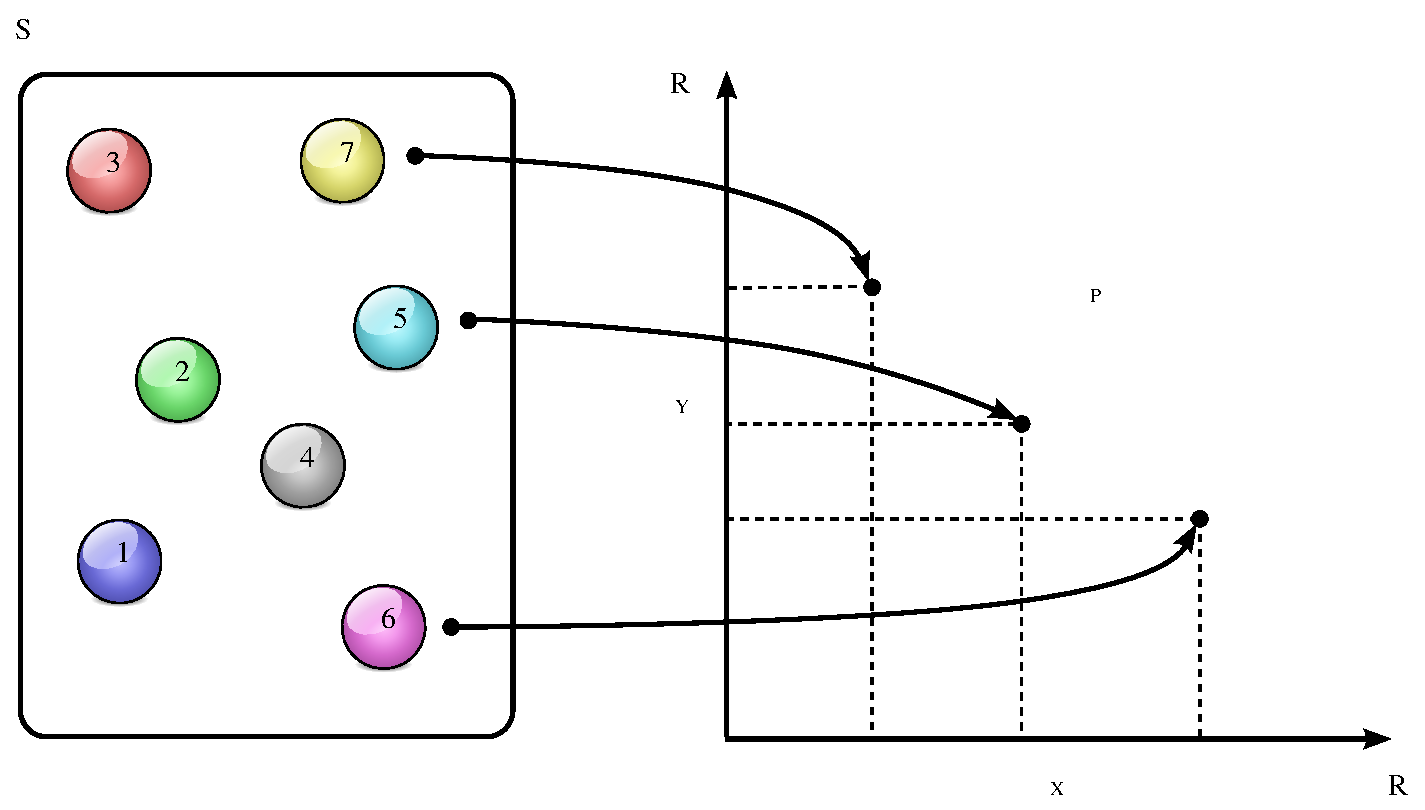
\includegraphics[width=11cm]{Figures/7Chapter/prv}
\end{psfrags}
\caption{The random pair $(X, Y)$ maps each outcome contained in the sample space to a real vector in $\RealNumbers^2$.}
\end{center}
\end{figure}

Suppose that $S$ is a subset of $X(\Omega) \times Y(\Omega)$.
We can express the probability of event $S$ as
\begin{equation*}
\begin{split}
\Pr (S) &= \Pr (\{ \omega \in \Omega | (X(\omega), Y(\omega)) \in S \}) \\
&= \sum_{(x,y) \in S} p_{X,Y} (x, y) .
\end{split}
\end{equation*}
In particular, we have
\begin{equation*}
\sum_{x \in X(\Omega)} \sum_{y \in Y(\Omega)} p_{X,Y} (x, y) = 1.
\end{equation*}

To further distinguish between the joint PMF of $X$ and $Y$ and the individual PMFs $p_X (\cdot)$ and $p_Y (\cdot)$, we occasionally refer to the latter as \emph{marginal probability mass functions}. \index{Probability mass function}
We can compute the marginal PMFs of $X$ and $Y$ from the joint PMF $p_{X,Y}$ using the formulas
\begin{align*}
p_X (x) &= \sum_{y \in Y(\Omega)} p_{X,Y} (x,y), \\
p_Y (y) &= \sum_{x \in X(\Omega)} p_{X,Y} (x,y).
\end{align*}
On the other hand, knowledge of the marginal PMFs $p_X (\cdot)$ and $p_Y (\cdot)$ is not sufficient to obtain a complete description of the joint PMF $p_{X,Y} (\cdot,\cdot)$.
Examples~\ref{example:JointPMFwoReplacement}~\&~\ref{example:JointPMFwithReplacement} illustrate the fact that knowledge of marginal PMFs is not sufficient to characterize the underlying joint PMF.

\begin{example} \label{example:JointPMFwoReplacement}
An urn contains three balls numbered one, two, and three.
A random experiment consists of drawing two balls from the urn, without replacement.
The number appearing on the first ball is a random variable, which we denote by $X$.
Similarly, we refer to the number inscribed on the second ball as $Y$.
The joint PMF of $X$ and $Y$ is given by
\begin{center}
\begin{tabular}{|c|c|c|c|}
\hline
$p_{X,Y} (x,y)$ & $1$ & $2$ & $3$ \\
\hline
$1$ & $0$ & $1/6$ & $1/6$ \\
\hline
$2$ & $1/6$ & $0$ & $1/6$ \\
\hline
$3$ & $1/6$ & $1/6$ & $0$ \\
\hline
\end{tabular}
\end{center}
We can compute the marginal PMF of $X$ as
\begin{equation*}
\begin{split}
p_X (x) &= \sum_{y \in Y(\Omega)} p_{X,Y} (x,y) \\
&= \frac{1}{6} + \frac{1}{6} = \frac{1}{3},
\end{split}
\end{equation*}
where $x \in \{1, 2, 3 \}$.
Likewise, the marginal PMF of $Y$ is seen to equal
\begin{equation*}
p_Y (y) = \left\{ \begin{array}{ll}
1/3, & \text{if }y \in \{ 1, 2, 3 \} \\
0, & \text{otherwise} .
\end{array} \right.
\end{equation*}
\end{example}

\begin{example} \label{example:JointPMFwithReplacement}
Again, suppose that an urn contains three balls numbered one, two and three.
This time the random experiment consists of drawing two balls from the urn with replacement.
We use $X$ and $Y$ to denote the numbers appearing on the first and second balls, respectively.
The joint PMF of $X$ and $Y$ is now equal to
\begin{center}
\begin{tabular}{|c|c|c|c|}
\hline
$p_{X,Y} (x,y)$ & $1$ & $2$ & $3$ \\
\hline
$1$ & $1/9$ & $1/9$ & $1/9$ \\
\hline
$2$ & $1/9$ & $1/9$ & $1/9$ \\
\hline
$3$ & $1/9$ & $1/9$ & $1/9$ \\
\hline
\end{tabular}
\end{center}
We can verify that the marginal PMF of $X$ and $Y$ are the same as in Example~\ref{example:JointPMFwoReplacement};
however, the joint PMFs differ.
\end{example}


\section{Functions and Expectations}

Let $X$ and $Y$ be two random variables with joint PMF $p_{X,Y} (\cdot, \cdot)$.
Consider a third random variable defined by $Z = g(X,Y)$, where $g : \RealNumbers^2 \mapsto \RealNumbers$ is a real-valued function.
We can obtain the PMF of $Z$ by computing
\begin{equation*}
p_Z (z)
= \sum_{\{ (x,y) | g(x,y) = z \}} p_{X,Y} (x, y).
\end{equation*}
This equation is the analog of \eqref{equation:FunctionPMF} for multiple random variables.

\begin{figure}[ht]
\begin{center}
\begin{psfrags}
\psfrag{1}[c]{$1$}
\psfrag{2}[c]{$2$}
\psfrag{3}[c]{$3$}
\psfrag{4}[c]{$4$}
\psfrag{5}[c]{$5$}
\psfrag{S}[l]{Sample Space}
\psfrag{R}[c]{$\RealNumbers$}
\psfrag{X}[c]{$X$}
\psfrag{Y}[c]{$Y$}
\psfrag{Z}[c]{$Z$}
\psfrag{g}[c]{$Z = g(X,Y)$}
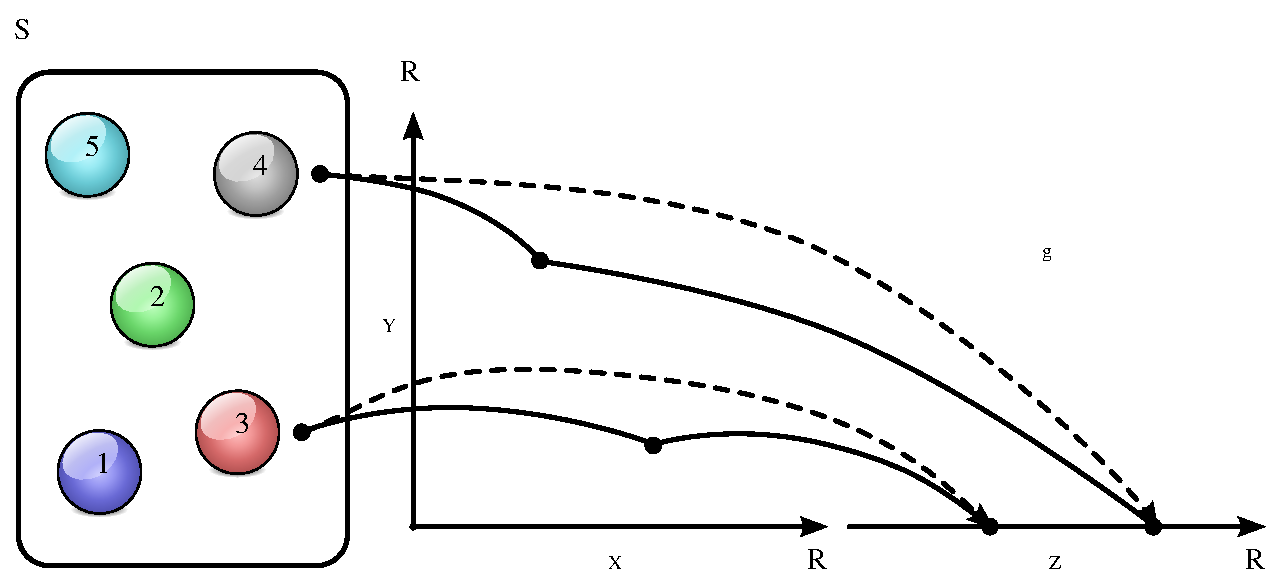
\includegraphics[width=11cm]{Figures/7Chapter/vfcn}
\end{psfrags}
\caption{A real-valued function of two random variables, $X$ and $Y$, is also a random variable.
Above, $Z = g(X, Y)$ maps outcomes in the sample space to real numbers.}
\end{center}
\end{figure}

\begin{example} \label{example:SumDice1}
Two dice, a blue die and a red one, are rolled simultaneously.
The random variable $X$ represents the number of dots that appears on the top face of the blue die, whereas $Y$ is equal to the number of dots on the red die.
We can form a random variable $Z$ that describes the sum of the two dice by defining $Z = X + Y$.
\end{example}

The definition of expectations can also be extended to multiple random variables.
In particular, the expected value of $g(X,Y)$ is obtained by computing
\begin{equation} \label{equation:ExpectationMultipleRV}
\Expect [g(X,Y)] = \sum_{x \in X(\Omega)} \sum_{y \in Y(\Omega)} g(x,y) p_{X,Y} (x,y) .
\end{equation}

\begin{example}
An urn contains three balls numbered one, two and three.
Two balls are selected from the urn at random, without replacement.
We employ $X$ to represent the number on the first ball and $Y$ for the number on the second ball.
We wish to compute the expected value of the function $X + Y$.

Using \eqref{equation:ExpectationMultipleRV}, we compute the expectation of $g(X,Y) = X + Y$ as
\begin{equation*}
\begin{split}
\Expect [g(X,Y)] &= \Expect [X + Y] \\
&= \sum_{x \in X(\Omega)} \sum_{y \in Y(\Omega)} (x + y) p_{X,Y} (x,y) \\
&= \sum_{x \in X(\Omega)} x p_X (x) + \sum_{y \in Y(\Omega)} y p_Y (y)
= 4.
\end{split}
\end{equation*}
The expected value of $X + Y$ is four.
\end{example}


\section{Conditional Random Variables}
\label{section:ConditionalRandomVariables}

Many random variables of practical interest are dependent.
That is, the realization of random variable $X$ may provide partial information about the random variable $Y$.
This inter-dependence is captured by the concept of conditioning, which was first discussed in Chapter~\ref{chapter:ConditionalProbability}.
In this section, we extend the concept of conditioning to multiple random variables.
We study the probability of events concerning random variable $Y$ given that some information about random variable $X$ is available.

Let $X$ and $Y$ be two random variables associated with the same experiment.
The \emph{conditional probability mass function} of $Y$ given $X = x$, denoted by $p_{Y|X} (\cdot | \cdot)$, is defined by \index{Conditional probability mass function}
\begin{equation*}
\begin{split}
p_{Y|X} (y|x) &= \Pr ( Y = y | X = x) \\
&= \frac{\Pr (\{Y = y\} \cap \{ X = x \})}{\Pr (X = x)} \\
&= \frac{ p_{X,Y} (x,y) }{p_X(x)},
\end{split}
\end{equation*}
provided that $p_X (x) \neq 0$.
Note that conditioning is not defined when $p_X (x)$ vanishes, as it has no meaning.
This is similar to conditional probability only being defined over events with non-zero probabilities.

Let $x$ be fixed with $p_X (x) > 0$.
The conditional PMF introduced above is a valid PMF since it is nonnegative and
\begin{equation*}
\begin{split}
\sum_{y \in Y(\Omega)} p_{Y|X} (y|x)
&= \sum_{y \in Y(\Omega)} \frac{p_{X,Y} (x,y)}{p_X (x)} \\
&= \frac{1}{p_X (x)} \sum_{y \in Y(\Omega)} p_{X,Y} (x,y) = 1.
\end{split}
\end{equation*}
The probability that $Y$ belongs to $S$ given $X = x$ is then obtained by summing the conditional probability $p_{Y|X} (\cdot | \cdot)$ over all outcomes included in $S$,
\begin{equation*}
\Pr (Y \in S | X = x) = \sum_{y \in S} p_{Y|X} (y | x) .
\end{equation*}

\begin{example}
Suppose that an urn contains three balls numbered one, two and three.
Two balls are drawn from this urn without replacement.
We wish to find the probability that the number on the second ball is odd.
We also wish to find the probability that the second ball is odd given that the number on the first ball is a three.

The probability that the number on the second ball is odd is given by the marginal distribution of the second  drawing, which was computed in Example~\ref{example:JointPMFwoReplacement}.
In the notation of that example, we have
\begin{equation*}
\Pr (Y \in \{1, 3\})
= p_Y (1) + p_Y (3)
= \frac{1}{3} + \frac{1}{3}
= \frac{2}{3} .
\end{equation*}
To compute the probability that the second ball is odd conditioned on the first ball being a three, we use the joint PMF derived in Example~\ref{example:JointPMFwoReplacement},
\begin{equation*}
\begin{split}
\Pr ( Y \in \{ 1, 3 \} | X = 3)
&= p_{Y|X}(1|3) + p_{Y|X}(3|3) \\
&= \frac{p_{X,Y}(1,3)}{p_X (3)} + \frac{p_{X,Y}(3,3)}{p_X (3)} \\
&= \frac{1/6}{1/3} + \frac{0}{1/3} = \frac{1}{2} .
\end{split}
\end{equation*}
The conditioning affects the probability of the second number drawn being odd.
\end{example}

The definition of conditional PMF can be rearranged to obtain a convenient formula to calculate the joint PMF of $X$ and $Y$, namely
\begin{equation*}
\begin{split}
p_{X,Y} (x,y) &= p_{Y|X} (y|x) p_X (x) \\
& = p_{X|Y} (x|y) p_Y (y) .
\end{split}
\end{equation*}
This formula can be use to compute the joint PMF of $X$ and $Y$ sequentially.

%\begin{example}
%\end{example}

It is also possible to define the conditional PMF of a random variable $X$, conditioned on an event $S$ where $\Pr (X \in S) > 0$.
Let $X$ be a random variable associated with a particular experiment, and let $S$ be a non-trivial event corresponding to this experiment.
The conditional PMF of $X$ given $S$ is defined by
\begin{equation} \label{equation:ConditionalEventPMF}
p_{X|S} (x) = \Pr (X = x | S)
= \frac{\Pr (\{X = x\} \cap S)}{\Pr (S)} .
\end{equation}
Note that the sets $\{ X = x \}$ form a partition of $\Omega$ as $x$ ranges over all the possible values in $X (\Omega)$.
By the total probability theorem, we deduce that
\begin{equation*}
\sum_{x \in X(\Omega)} \Pr ( \{X = x\} \cap S) = \Pr (S)
\end{equation*}
and, consequently, we get
\begin{equation*}
\sum_{x \in X(\Omega)} p_{X|S} (x) = 1 .
\end{equation*}
Hence, we conclude that $p_{X|S} (\cdot)$ is a valid PMF.

\begin{example}[Splitting Property of Poisson PMF]
A digital communication system transmits out either a one with probability $p$ or a zero with probability $1 - p$, independently of previous transmissions.
The number of transmitted binary digits within a given time interval has a Poisson PMF with parameter $\lambda$.
We wish to show that the number of ones sent in that same time interval has a Poisson PMF with parameter $p \lambda$.

Let $M$ denote the number of ones within the stipulated interval, $N$ be the number of zeros, and $K = M + N$ be the total number of transmissions during the same interval.
The number of ones given that the total number of transmissions is $k$ is given by
\begin{equation*}
p_{M|K} (m | k) = \binom{k}{m} p^m (1-p)^{k - m},
\quad m = 0, 1, \ldots, k.
\end{equation*}
The probability that $M$ is equal to $m$ is therefore equal to
\begin{equation*}
\begin{split}
p_{M} (m) &= \sum_{k = 0}^{\infty} p_{M|K} (m | k) p_K(k) \\
&= \sum_{k = m}^{\infty} \binom{k}{m} p^m (1-p)^{k - m}
\frac{\lambda^{k}}{k !} e^{-\lambda} \\
&= \sum_{u = 0}^{\infty} \binom{u+m}{m} p^m (1-p)^{u}
\frac{\lambda^{u+m}}{(u+m)!} e^{-\lambda} \\
&= \frac{(\lambda p)^m}{m!} e^{-\lambda}
\sum_{u = 0}^{\infty} \frac{( (1-p) \lambda)^{u}}{u!}
= \frac{(\lambda p)^m}{m!} e^{-p \lambda} .
\end{split}
\end{equation*}
Above, we have used the change of variables $k = u+m$.
We have also rearranged the sum into a familiar form, leveraging the fact that the summation of a Poisson PMF over all its possible values is equal to one.
We can see that $M$ has a Poisson PMF with parameter $p \lambda$.
\end{example}


\section{Conditional Expectations}

The \emph{conditional expectation} of $Y$ given $X = x$ is simply the expectation of $Y$ with respect to the conditional PMF $p_{Y|X} (\cdot | \cdot)$, \index{Conditional expectation}
\begin{equation*}
\Expect [Y | X = x ] = \sum_{y \in Y(\Omega)} y p_{Y|X} (y|x).
\end{equation*}
This conditional expectation can be viewed as a function of $x$,
\begin{equation*}
h(x) = \Expect [Y | X = x] .
\end{equation*}
It is therefore mathematically accurate and sometimes desirable to talk about the random variable $h (X) = \Expect [Y | X]$.
Let $X$ and $Y$ be two random variables associated with an experiment.
The outcome of this experiment determines the value of $X$, say $X = x$, which in turn produces the value $h(x) = \Expect [Y | X = x]$.
In this sense, a conditional expectation is simply a special random variable.

Not too surprisingly, the expectation of $\Expect [Y | X]$ is given by
\begin{equation*}
\begin{split}
\Expect \left[ \Expect [Y | X] \right]
&= \sum_{x \in X(\Omega)} \Expect [Y | X = x] p_X (x) \\
&= \sum_{x \in X(\Omega)} \sum_{y \in Y(\Omega)} y p_{Y|X} (y|x) p_X (x) \\
&= \sum_{y \in Y(\Omega)} \sum_{x \in X(\Omega)} y p_{X,Y} (x, y) \\
%&= \sum_{y \in Y(\Omega)} y \sum_{x \in X(\Omega)} p_{X,Y} (x, y) \\
&= \sum_{y \in Y(\Omega)} y p_{Y} (y)
= \Expect [Y] .
\end{split}
\end{equation*}
Using a similar argument, it is straightforward to show that
\begin{equation*}
\Expect \left[ \Expect [g (Y) | X] \right] = \Expect [g(Y)] .
\end{equation*}

\begin{example}
An entrepreneur opens a small business that sells two kinds of beverages from the Brazos Soda Company, cherry soda and lemonade.
The number of bottles sold in an hour at the store is found to be a Poisson random variable with parameter $\lambda = 10$.
Every customer selects a cherry soda with probability $p$ and a lemonade with probability $(1 - p)$, independently of other customers.
We wish to find the conditional mean of the number of cherry sodas purchased in an hour given that a total of ten beverages was purchased by customers during that time period.

Let $B$ represent the number of bottles sold during an hour.
Similarly, let $C$ and $L$ be the number of cherry sodas and lemonades purchased during that hour, respectively.
We note that $B = C + L$.
The conditional PMF of $C$ given that the total number of beverages sold equals ten ($B = 10$) is
\begin{equation} \label{equation:ConditionalPoisson}
p_{C|B} (k | 10)
= \binom{10}{k} p^k (1-p)^{10-k} .
\end{equation}
This follows from the fact that every customer selects a cherry soda with probability $p$, independently of other customers.
The conditional mean is then seen to equal
\begin{equation*}
\Expect [ C | B=10] = \sum_{k=0}^{10}
k \binom{10}{k} p^k (1-p)^{10-k} = 10 p .
\end{equation*}
\end{example}

We can define the expectation of $X$ conditioned on event $S$ in an analogous manner.
Let $S$ be an event such that $\Pr (S) > 0$.
The conditional expectation of $X$ given $S$ is
\begin{equation*}
\Expect [X | S] = \sum_{x \in X(\Omega)} x p_{X|S} (x) ,
\end{equation*}
where $p_{X|S} (\cdot)$ is as defined in \eqref{equation:ConditionalEventPMF}.
Similarly, we have
\begin{equation*}
\Expect [g(X) | S] = \sum_{x \in X(\Omega)} g(x) p_{X|S} (x) ,
\end{equation*}

\begin{example}
Spring break is coming and a student decides to renew his shirt collection.
The number of shirts purchased by the student is a random variable denoted by $N$.
The PMF of this random variable is a geometric distribution with parameter $p = 0.5$.
Any one shirt costs \$10, \$20 or \$50 with respective probabilities 0.5, 0.3 and 0.2, independently of other shirts.
We wish to compute the expected amount of money spent by the student.
Also, we wish to compute the expected amount of money disbursed given that the student buys at least five shirts.

Let $C_i$ be the cost of the $i$th shirt.
The total amount of money spent by the student, denoted by $T$, can be expressed as
\begin{equation*}
T = \sum_{i=1}^N C_i .
\end{equation*}
The mean of $T$ can be computed using nested expectation.
It is equal to
\begin{equation*}
\begin{split}
\Expect [T] = \Expect \left[ \sum_{i=1}^N C_i \right]
&= \Expect \left[ \Expect \left[
\sum_{i=1}^N C_i \Big| N \right] \right] \\
&= \Expect \left[ \sum_{i=1}^N \Expect [ C_i | N ] \right] \\
&= 21 \Expect [ N ] = 42.
\end{split}
\end{equation*}
The student is expected to spend \$42.
Given that the student buys at least five shirts, the conditional expectation becomes
\begin{equation*}
\begin{split}
\Expect [T | N \geq 5]
&= \Expect \left[ \sum_{i=1}^N C_i \Big| N \geq 5 \right] \\
&= \Expect \left[ \Expect \left[
\sum_{i=1}^N C_i \Big| N \right] \bigg| N \geq 5 \right] \\
&= 21 \Expect [ N | N \geq 5] \\
&= 21 \sum_{n=5}^{\infty} n p_{N | N \geq 5} (n)
= 126 .
\end{split}
\end{equation*}
Condition on buying more than five shirts, the student is expected to spend \$126.
In computing the conditional expectation, we have use the memoryless property of the geometric random variable.
\end{example}


\section{Independence}

Let $X$ and $Y$ be two random variables associated with one experiment.
We say that $X$ and $Y$ are \emph{independent random variables} if \index{Independence}
\begin{equation*}
p_{X,Y} (x,y) = p_X (x) p_Y (y)
\end{equation*}
for every $x \in X(\Omega)$ and every $y \in Y(\Omega)$.

There is a clear relation between the concept of independence introduced in Section~\ref{section:Independence} and the independence of two random variables.
Two random variables are independent if and only if the events $\{ X = x \}$ and $\{ Y = y \}$ are independent for every $x \in X(\Omega)$ and every $y \in Y(\Omega)$.

\begin{theorem}
If $X$ and $Y$ are independent random variables, then
\begin{equation*}
\Expect [X Y] = \Expect [X] \Expect [Y] .
\end{equation*}
\end{theorem}
\begin{proof}
Assume that both $\Expect [X]$ and $\Expect[Y]$ exist, then
\begin{equation*}
\begin{split}
\Expect [XY]
&= \sum_{x \in X(\Omega)} \sum_{y \in Y(\Omega)} x y p_{X,Y} (x,y) \\
&= \sum_{x \in X(\Omega)} \sum_{y \in Y(\Omega)} x y p_X (x) p_Y (y) \\
&= \sum_{x \in X(\Omega)} x p_X (x) \sum_{y \in Y(\Omega)} y p_Y (y)
= \Expect [X] \Expect [Y] ,
\end{split}
\end{equation*}
where we have used the fact that $p_{X,Y} (x,y) = p_X (x) p_Y (y)$ for independent random variables.
\end{proof}

\begin{example}
Two dice of different colors are rolled, as in Example~\ref{example:SumDice1}.
We wish to compute the expected value of their product.
We know that the mean of each role is $\Expect [X] = \Expect [Y] = 3.5$.
Furthermore, it is easy to show that $X$ and $Y$, the numbers of dots on the two dice, are independent random variable.
The expected value of their product is then equal to the product of the individual means, $\Expect [XY] = \Expect [X] \Expect [Y] = 12.25$.
\end{example}

A similar argument can be used to show that
\begin{equation} \label{equation:DiscreteProduct}
\Expect[ g(X) h(Y) ] = \Expect [ g(X) ] \Expect [ h(Y) ]
\end{equation}
whenever $X$ and $Y$ are independent random variables and the corresponding expectations exist.

One intesting application of \eqref{equation:DiscreteProduct} occurs when taking the sum of independent random variables.
Let $X$ and $Y$ be two independent random variables that take on integer values, and define $U = X + Y$.
The ordinary generating function of $U$, as defined in Section~\ref{section:OrdinaryGeneratingFunctions}, is given by
\begin{equation*}
\begin{split}
G_U (z) &= \Expect \left[ z^U \right]
= \Expect \left[ z^{X + Y} \right] \\
&= \Expect \left[ z^X z^Y \right]
= \Expect \left[ z^X \right] \Expect \left[ z^Y \right] \\
&= G_X(z) G_Y(z) .
\end{split}
\end{equation*}
That is, the generating function of a sum of independent random variables is equal to the product of the individual ordinary generating functions, provided that the latter both exist.

\begin{example}
Let $X$ be a Poisson random variable with parameter $\alpha$ and, similarly, let $Y$ be a Poisson random variable with parameter $\beta$.
We wish to find the probability mass function of $U = X + Y$.

To solve this problem, we use ordinary generating functions.
First, we compute the generating function of $X$,
\begin{equation*}
\begin{split}
G_X (z) &= \Expect \left[ z^X \right]
= \sum_{k=0}^{\infty} \frac{\alpha^k}{k!} e^{-\alpha} z^k \\
&= e^{-\alpha} \sum_{k=0}^{\infty} \frac{(\alpha z)^k}{k!}
= e^{-\alpha} e^{\alpha z} = e^{\alpha (z-1)} .
\end{split}
\end{equation*}
By analogy, we also have $G_Y (z) = e^{\beta (z-1)}$.
The ordinary generating function of $U = X + Y$ then becomes
\begin{equation*}
G_U (z) = G_X (z) G_Y(z) = e^{\alpha (z-1)} e^{\beta (z-1)}
= e^{(\alpha + \beta) (z-1)} .
\end{equation*}
We conclude, by the uniqueness of generating functions, that $U$ is a Poisson random variable with parameter $\alpha + \beta$ and, accordingly, we get
\begin{equation*}
p_U (k) = \frac{ (\alpha + \beta)^k }{k!} e^{- (\alpha + \beta) }, \quad k = 0, 1, 2, \ldots
\end{equation*}
\end{example}

We saw in Section~\ref{section:ConditionalRandomVariables} that a random variable can also be conditioned on a specific event.
Let $X$ be a random variable and let $S$ be a non-trivial event.
The variable $X$ is \emph{independent} of $S$ if
\begin{equation*}
\Pr (\{X = x \} \cap S ) = p_X (x) \Pr (S)
\end{equation*}
for every $x \in X(\Omega)$.
In particular, if $X$ is independent of event $S$ then
\begin{equation*}
p_{X|S} (x) = p_X (x)
\end{equation*}
for all $x \in X(\Omega)$.



%\setcounter{page}{89}
%\setcounter{chapter}{7}
%\part{Continuous Random Variables}
%\chapter{Continuous Random Variables}

In our previous discussion, we introduced discrete random variables and discussed their properties.
Discrete random variables are quite useful in many contexts, yet they form only a small subset of the collection of random variables pertinent to applied probability and engineering.
In this chapter, we consider random variables that range over a continuum of possible values; that is, random variables that can take on an uncountable set of values.

Continuous random variables are powerful mathematical abstractions that allow practitioners to pose and solve important engineering problems, which cannot be addressed using discrete models.
While this extra flexibility is useful and desirable, it comes at a certain cost.
A continuous random variable cannot be characterized by a probability mass function.
This difficulty emerges from the limitations of the third axiom of probability laws, which only applies to countable collections of disjoint events.

Below, we provide a definition for continuous random variables.
Furthermore, we extend and apply the concepts and methods initially developed for discrete random variables to the class of continuous random variables.
In particular, we develop a continuous counterpart to the probability mass function.


\section{Cumulative Distribution Functions}

We begin our exposition of continuous random variables by introducing a general concept which can be employed to bridge our understanding of discrete and continuous random variables.
Recall that a \emph{random variable} is a real-valued function acting on the outcomes of an experiment. \index{Random variable}
In particular, given a sample space, random variable $X$ is a function from $\Omega$ to $\RealNumbers$.
The \emph{cumulative distribution function (CDF)} of $X$ is defined point-wise as the probability of the event $\{X \leq x \}$, \index{Cumulative distribution function}
\begin{equation*}
F_X (x) = \Pr ( \{ X \leq x \} ) = \Pr (X \leq x).
\end{equation*}
In terms of the underlying sample space, $F_X (x)$ denotes the probability of the set of all outcomes in $\Omega$ for which the value of $X$ is less than or equal to $x$,
\begin{equation*}
F_X (x) = \Pr \left( X^{-1} ( (- \infty, x]) \right)
= \Pr (\{ \omega \in \Omega | X(\omega) \leq x \}).
\end{equation*}
In essence, the CDF is a convenient way to specify the probability of all events of the form $\{ X \in (-\infty, x] \}$.

The CDF of random variable $X$ exists for any well-behaved function $X : \Omega \mapsto \RealNumbers$.
Moreover, since the realization of $X$ is a real number, we have
\begin{gather*}
\lim_{x \downarrow - \infty} F_X (x) = 0 \\
\lim_{x \uparrow \infty} F_X (x) = 1.
\end{gather*}
Suppose $x_1 < x_2$, then we can write $\{ X \leq x_2 \}$ as the union of the two disjoint sets $\{ X \leq x_1 \}$ and $\{ x_1 < X \leq x_2 \}$.
It follows that
\begin{equation} \label{equation:NonDecreasingCDF}
\begin{split}
F_X (x_2) &= \Pr (X \leq x_2) \\
&= \Pr (X \leq x_1) + \Pr (x_1 < X \leq x_2) \\
&\geq \Pr (X \leq x_1) = F_X (x_1).
\end{split}
\end{equation}
In other words, a CDF is always a non-decreasing function.
Finally, we note from \eqref{equation:NonDecreasingCDF} that the probability of $X$ falling in the interval $(x_1, x_2]$ is
\begin{equation} \label{equation:IntervalCDF}
\Pr (x_1 < X \leq x_2) = F_X (x_2) - F_X (x_1).
\end{equation}


\subsection{Discrete Random Variables}

If $X$ is a discrete random variable, then the CDF of $X$ is given by
\begin{equation*}
F_X (x) = \sum_{u \in X(\Omega) \cap (-\infty, x]} p_X (u),
\end{equation*}
and its PMF can be computed using the formula
\begin{equation*}
p_X (x) = \Pr (X \leq x) - \Pr (X < x) = F_X (x) - \lim_{u \uparrow x} F_X (u).
\end{equation*}
Fortunately, this formula is simpler when the random variable $X$ only takes integer values, as seen in the example below.

\begin{figure}[ht]
\begin{center}
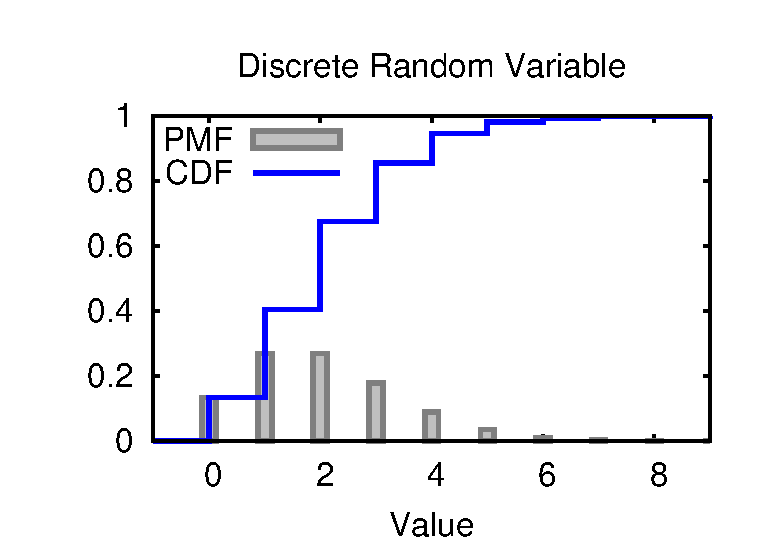
\includegraphics[width=8.5cm]{Figures/8chapter/discrete_cdf}
\end{center}
\caption{This figure shows the PMF of a discrete random variable, along with the corresponding CDF.
The values of the PMF are depicted by the height of the rectangles; their cumulative sums lead to the values of the CDF.}
\end{figure}

\begin{example}
Let $X$ be a geometric random variable with parameter $p$,
\begin{equation*}
p_X (k) = (1 - p)^{k-1} p \quad k = 1, 2, \ldots 
\end{equation*}
For $x > 0$, the CDF of $X$ is given by
\begin{equation*}
F_X (x) = \sum_{k = 1}^{\lfloor x \rfloor} (1 - p)^{k-1} p
= 1 - (1 - p)^{\lfloor x \rfloor} ,
\end{equation*}
where $\lfloor \cdot \rfloor$ is the standard floor function.
For integer $k \geq 1$, the PMF of geometric random variable $X$ can be recovered from the CDF as follows,
\begin{equation*}
\begin{split}
p_X (k) &= F_X (x) - \lim_{u \uparrow x} F_X (u) = F_X (k) - F_X (k-1) \\
&= \left( 1 - (1-p)^k \right) - \left( 1 - (1-p)^{k-1} \right) \\
%&= (1 - p)^{k-1} - (1-p) (1-p)^{k-1} \\
&= (1 - p)^{k-1} p .
\end{split}
\end{equation*}
\end{example}


\subsection{Continuous Random Variables}

Having defined the concept of a CDF, we can safely provide a more precise definition for continuous random variables.
Let $X$ be a random variable with CDF $F_X (x)$, then $X$ is said to be a \emph{continuous random variable} if $F_X (x)$ is differentiable with respect to $x$. \index{Continuous random variable}

\begin{example}
Suppose that $X$ is a random variable with CDF given by
\begin{equation*}
F_X(x) = \begin{cases} 1 - e^{-x}, & x \geq 0 \\
0, & x < 0 . \end{cases}
\end{equation*}
This cumulative distribution function is differentiable with
\begin{equation*}
\frac{dF_X}{dx}(x)
= \begin{cases} e^{-x}, & x \geq 0 \\
0, & x < 0 \end{cases}
\end{equation*}
and therefore $X$ is a continuous random variable.
\end{example}

\begin{figure}[ht]
\begin{center}
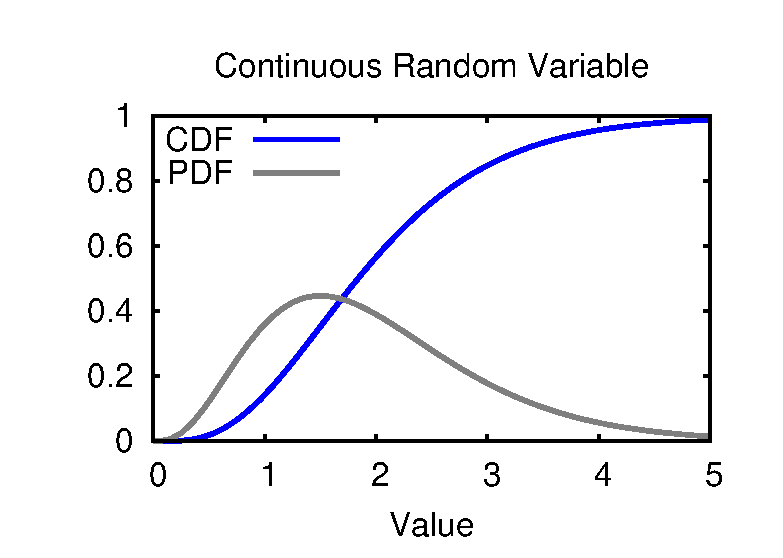
\includegraphics[width=8.5cm]{Figures/8chapter/continuous_cdf}
\end{center}
\caption{The CDF of a continuous random variable is differentiable.
This figure provides one example of a continuous random variable.
Both, the CDF $F_X(\cdot)$ and its derivative $f_X(\cdot)$ (PDF) are displayed.}
\end{figure}


\subsection{Mixed Random Variables*}

Generally speaking, the CDF of a discrete random variable is a discontinuous staircase-like function, whereas the CDF of a continuous random variable is continuous and differentiable almost everywhere.
There exist random variables for which neither of these two situations apply.
Such random variables are sometimes called \emph{mixed random variables}. \index{Mixed random variable}
Our exposition of mixed random variables in this document is very limited.
Still, we emphasize that a good understanding of discrete and continuous random variables is instrumental in understanding and solving problems with mixed random variables.

\begin{figure}[ht]
\begin{center}
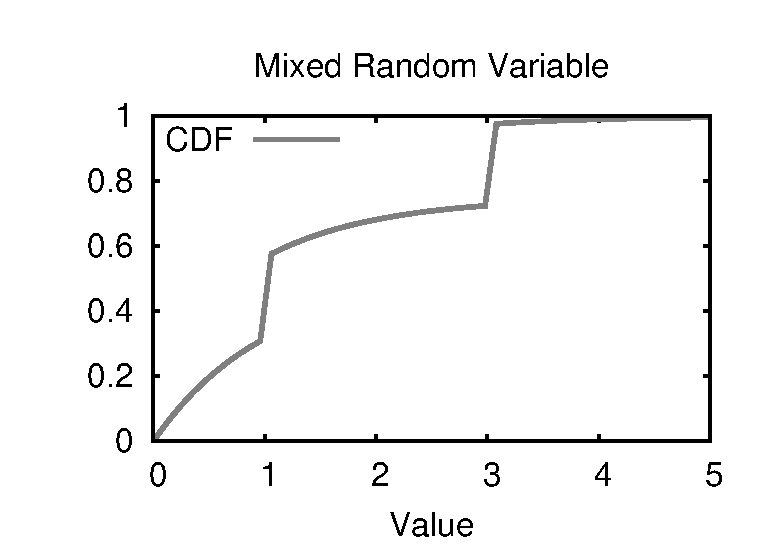
\includegraphics[width=8.5cm]{Figures/8chapter/mixed_cdf}
\end{center}
\caption{This figure shows the CDF of a mixed random variable.
In general, mixed random variables do not have a PMF or a PDF.
Their CDF may be composed of a mixture of differentiable intervals and discontinuous jumps.}
\end{figure}


\section{Probability Density Functions}

As mentioned above, the CDF of continuous random variable $X$ is a differentiable function.
The derivative of $F_X (\cdot)$ is called the \emph{probability density function (PDF)} of $X$, and it is denoted by $f_X(\cdot)$. \index{Probability density function (PDF)}
If $X$ is a random variable with PDF $f_X (x)$ then, by the fundamental theorem of calculus, we have
\begin{equation*}
F_X (x) = \int_{- \infty}^x f_X (\xi) d\xi .
\end{equation*}
Equivalently, we can write
\begin{equation*}
f_X (x) = \frac{d F_X}{dx} (x) .
\end{equation*}
Note that PDFs are only defined for continuous random variables.
This is somewhat restrictive.
Still, the PDF is a very powerful tool that can be employed to derive properties of continuous random variables which would be difficult to compute otherwise.

For $x_1 < x_2$, we can combine the definition of $f_X(\cdot)$ and \eqref{equation:IntervalCDF} to obtain
\begin{equation*}
\Pr (x_1 < X \leq x_2) = \int_{x_1}^{x_2} f_X (\xi) d\xi .
\end{equation*}
Furthermore, it is easily seen that for any continuous random variable
\begin{equation*}
\begin{split}
\Pr (X = x_2) &= \lim_{x_1 \uparrow x_2} \Pr (x_1 < X \leq x_2)
= \lim_{x_1 \uparrow x_2} \int_{x_1}^{x_2} f_X (\xi) d\xi \\
&= \int_{x_2}^{x_2} f_X (\xi) d\xi = 0.
\end{split}
\end{equation*}
In other words, if $X$ is a continuous random variable, then $\Pr (X = x) = 0$ for any real number $x$.
An immediate corollary of this fact is
\begin{equation*}
\begin{split}
\Pr (x_1 < X < x_2)
&= \Pr (x_1 \leq X < x_2)
= \Pr (x_1 < X \leq x_2) \\
&= \Pr (x_1 \leq X \leq x_2) ;
\end{split}
\end{equation*}
the inclusion or exclusion of endpoints in an interval does not affect the probability of the corresponding interval when $X$ is a continuous random variable.

We can derive properties for the PDF of continuous random variable $X$ based on the axioms of probability laws.
First, the probability that $X$ is a real number is given by
\begin{equation*}
\Pr (-\infty < X < \infty) = \int_{-\infty}^{\infty} f_X (\xi) d\xi = 1.
\end{equation*}
Thus, $f_X (x)$ must integrate to one.
Also, because the probabilities of events are nonnegative, we must have $f_X (x) \geq 0$ everywhere.
Finally, given an admissible set $S$, the probability that $X \in S$ can be expressed through an integral,
\begin{equation*}
\Pr (X \in S) = \int_S f_X (\xi) d\xi .
\end{equation*}


\section{Important Distributions}

Good intuition about continuous random variables can be developed by looking at examples.
In this section, we introduce important random variables and their distributions.
These random variables find widespread application in various fields of engineering.


\subsection{The Uniform Distribution}

A (continuous) \emph{uniform random variable} is such that all intervals of the same length contained within its support are equally probable. \index{Uniform random variable (continuous)}
The PDF of a uniform random variable is defined by two parameters, $a$ and $b$, which are its minimum and maximum possible values, respectively.
The PDF $f_X(x)$ is given by
\begin{equation*}
f_X(x) = \begin{cases} \frac{1}{b-a}, & x \in [a, b] \\
0, & \text{otherwise}. \end{cases}
\end{equation*}
The associated cumulative distribution function becomes
\begin{equation*}
F_X(x) = \begin{cases} 0, & x < a \\
\frac{x-a}{b-a}, & a \leq x \leq b \\
1, & x \geq b . \end{cases}
\end{equation*}

\begin{figure}[ht]
\begin{center}
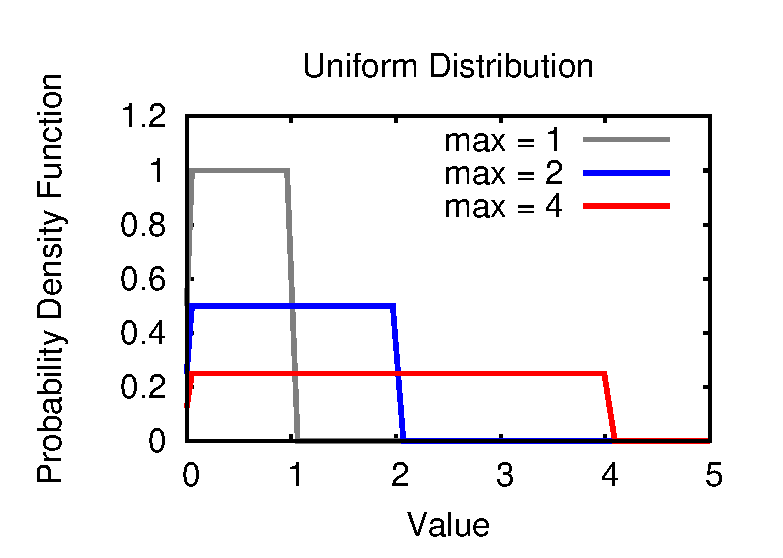
\includegraphics[width=8.5cm]{Figures/8chapter/uniform_pdf}
\end{center}
\caption{This figure shows the PDFs of uniform random variables with support intervals $[0,1]$, $[0,2]$ and $[0,4]$.}
\end{figure}

\begin{example}
David comes to campus every morning using the Aggie Spirit Transit.
On his route, a bus comes every thirty minutes, from sunrise until sunset.
David, who does not believe in alarm clocks or watches, wakes up with daylight.
After cooking a hefty breakfast, he walks to the bus stop.
If his arrival time at the bus stop is uniformly distributed between 9:00 a.m.\ and 9:30 a.m., what is the probability that he waits less than five minutes for the bus?

Let $t_0$ be the time at which David arrives at the bus stop, and denote by $T$ the time he spends waiting.
The time at which the next bus arrives at David's stop is uniformly distributed between $t_0$ and $t_0 + 30$.
The amount of time that he spends at the bus stop is therefore uniformly distributed between $0$ and $30$ minutes.
Accordingly, we have
\begin{equation*}
f_T(t) = \begin{cases} \frac{1}{30}, & t \in [0, 30] \\
0, & \text{otherwise}. \end{cases}
\end{equation*}
The probability that David waits less than five minutes is
\begin{equation*}
\Pr (T < 5) = \int_0^5 \frac{1}{30} dt = \frac{1}{6} .
\end{equation*}
\end{example}


\subsection{The Gaussian (Normal) Random Variable}

The \emph{Gaussian random variable} is of fundamental importance in probability and statistics. \index{Gaussian random variable}
It is often used to model the distribution of a sum of random components.
The PDF of a Gaussian random variable is given by
\begin{equation*}
f_X (x) = \frac{1}{\sqrt{2 \pi} \sigma} e^{- \frac{(x - m)^2}{2 \sigma^2}}
\quad - \infty < x < \infty,
\end{equation*}
where $m$ and $\sigma > 0$ are real parameters.

\begin{figure}[ht]
\begin{center}
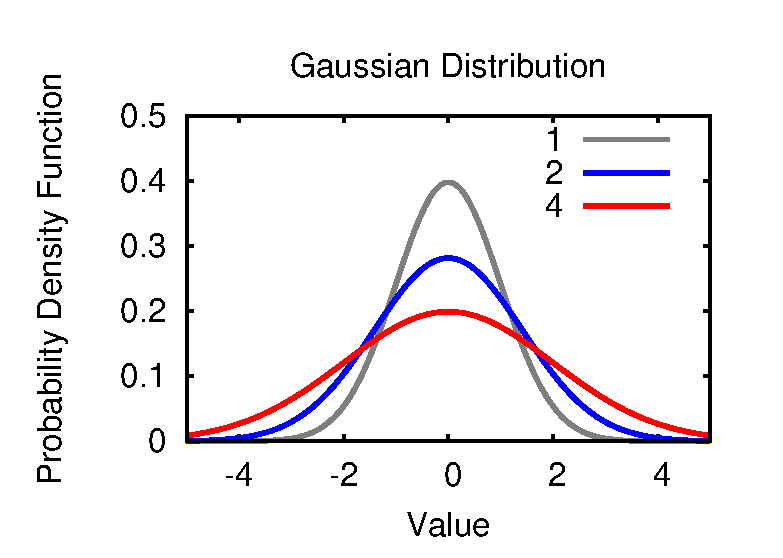
\includegraphics[width=8.5cm]{Figures/8chapter/gaussian_pdf}
\end{center}
\caption{The distributions of Gaussian random variables appear above for parameters $m = 0$ and $\sigma^2 \in \{ 1, 2, 4 \}$.}
\end{figure}

A Gaussian random variable whose distribution has parameters $m = 0$ and $\sigma = 1$ is called a \emph{normal random variable}, a name that hints at its popularity. \index{Normal random variable}
The CDF of a Gaussian random variable does not admit a closed-form expression; it can be expressed as
\begin{equation*}
\begin{split}
F_X (x) &= \Pr (X \leq x)
= \frac{1}{\sqrt{2 \pi} \sigma}
\int_{- \infty}^{x} e^{- \frac{(\xi - m)^2}{2 \sigma^2}} d\xi \\
&= \frac{1}{\sqrt{2 \pi}}
\int_{- \infty}^{(x - m)/\sigma} e^{- \frac{\zeta^2}{2}} d\zeta
= \Phi \left( \frac{x - m}{\sigma} \right),
\end{split}
\end{equation*}
where $\Phi (\cdot)$ is termed the \emph{standard normal cumulative distribution function} and is defined by
\begin{equation*}
\Phi (x) = 
\frac{1}{\sqrt{2 \pi}} \int_{-\infty}^x e^{-\frac{\zeta^2}{2}} d\zeta .
\end{equation*}
We emphasize that the function $\Phi (\cdot)$ is nothing more than a convenient notation for the CDF of a normal random variable.

\begin{example} \label{example:NoiseCommunicationSystem1}
A binary signal is transmitted through a noisy communication channel.
The sent signal takes on either a value of $1$ or $-1$.
The message received at the output of the communication channel is corrupted by additive thermal noise.
This noise can be accurately modeled as a Gaussian random variable.
The receiver declares that a $1$ ($-1$) was transmitted if the sent signal is positive (negative).
What is the probability of making an erroneous decision?

Let $S \in \{ -1, 1 \}$ denote the transmitted signal, $N$ be the value of the thermal noise, and $Y$ represent the value of the received signal.
An error can occur in one of two possible ways: $S = 1$ was transmitted and $Y$ is less than zero, or $S = -1$ was transmitted and $Y$ is greater than zero.
Using the total probability theorem, we get can compute the probability of error as
\begin{equation*}
\Pr (Y \geq 0 | S = -1) \Pr (S = -1)
+ \Pr (Y \leq 0 | S = 1) \Pr (S = 1).
\end{equation*}
By symmetry, it is easily argued that
\begin{equation*}
\begin{split}
\Pr (Y \leq 0 | S = 1) &= \Pr (Y \geq 0 | S = -1) = \Pr (N > 1) \\
&= \int_{1}^{\infty} \frac{1}{\sqrt{2 \pi} \sigma}
e^{- \frac{\xi^2}{2 \sigma^2}} d\xi
= 1 - \Phi \left( \frac{1}{\sigma} \right) .
\end{split}
\end{equation*}
The probability that the receiver makes an erroneous decision is $1 - \Phi (1/\sigma)$.
Clearly, the reliability of this transmission scheme depends on the amount of noise present at the receiver.
\end{example}

The normal random variable is so frequent in applied mathematics and engineering that many variations of its CDF possess their own names.
The \emph{error function} is a function which is primarily encountered in the fields of statistics and partial differential equations. \index{Error function}
It is defined by
\begin{equation*}
\mathrm{erf} (x) = \frac{2}{\sqrt{\pi}} \int_0^x e^{-\xi^2} d\xi .
\end{equation*}
The error function is related to the standard normal cumulative distribution function by scaling and translation,
\begin{equation*}
\Phi (x) = \frac{1 + \mathrm{erf} \left( {x}/{\sqrt{2}} \right)}{2}.
\end{equation*}
If $X$ is a standard normal random variable, then $\mathrm{erf} \left( x/{\sqrt{2}} \right)$ denotes the probability that $X$ lies in the interval $(-x, x)$.
In engineering, it is customary to employ the \emph{$Q$-function}, which is given by \index{Q-function}
\begin{equation} \label{equation:Qfunction}
\begin{split}
Q (x) &= \frac{1}{\sqrt{2 \pi}} \int_x^{\infty} e^{-\frac{\xi^2}{2}} d\xi
= 1 - \Phi (x) \\
&= \frac{ 1 - \mathrm{erf} \left( {x}/{\sqrt{2}} \right) }{2} .
\end{split}
\end{equation}
Equation \eqref{equation:Qfunction} may prove useful when using software packages that provide a built-in implementation for $\mathrm{erf}(\cdot)$, but not for the $Q$-function.
The probability of an erroneous decision in Example~\ref{example:NoiseCommunicationSystem1} can be expressed concisely using the Q-function as $Q (1/\sigma)$.


Next, we prove that the standard normal PDF integrates to one.
The solution is easy to follow, but hard to discover.
It is therefore useful to include it here.
Consider a standard normal PDF,
\begin{equation*}
f_X(x) = \frac{1}{\sqrt{2 \pi}} e^{- \frac{x^2}{2}} .
\end{equation*}
We can show that $f_X (x)$ integrates to one using a subtle argument and a change of variables.
We start with the square of the integrated PDF and proceed from there,
\begin{equation*}
\begin{split}
\left(\int_{- \infty}^{\infty} f_X (\xi) d\xi \right)^2
&= \int_{- \infty}^{\infty} \frac{1}{\sqrt{2 \pi}} e^{- \frac{\xi^2}{2}} d\xi
\int_{- \infty}^{\infty} \frac{1}{\sqrt{2 \pi}} e^{- \frac{\zeta^2}{2}} d\zeta \\
&= \int_{- \infty}^{\infty} \int_{- \infty}^{\infty}
\frac{1}{2 \pi} e^{- \frac{\xi^2 + \zeta^2}{2}} d\xi d\zeta
= \int_{0}^{2 \pi} \frac{1}{2 \pi} d\theta
\int_{0}^{\infty} e^{- \frac{r^2}{2}} r dr \\
&= \left. \left( - e^{- \frac{r^2}{2}} \right) \right|_0^{\infty} = 1.
\end{split}
\end{equation*}
Since the square of the desired integral is nonnegative and equal to one, we can conclude that the normal PDF integrates to one.


\subsection{The Exponential Distribution}
\label{section:ExponentialDistribution}

The \emph{exponential random variable} is also frequently encountered in engineering. \index{Exponential random variable}
It can be used to model the lifetime of devices and systems, and the time elapsed between specific occurrences.
An exponential random variable $X$ with parameter $\lambda > 0$ has PDF
\begin{equation*}
f_X (x) = \lambda e^{- \lambda x} \quad x \geq 0.
\end{equation*}
For $x \geq 0$, its CDF is equal to
\begin{equation*}
F_X (x) = 1 - e^{- \lambda x} .
\end{equation*}
The parameter $\lambda$ characterizes the rate at  which events occur.

\begin{figure}[ht]
\begin{center}
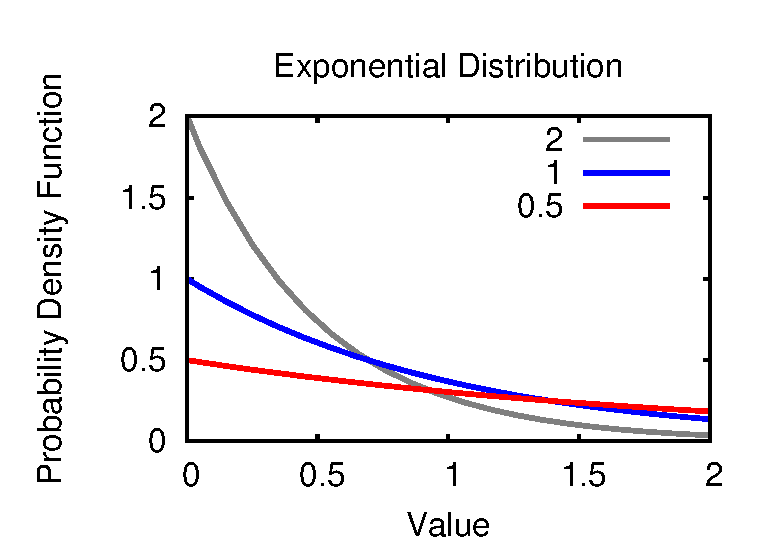
\includegraphics[width=8.5cm]{Figures/8chapter/exponential_pdf}
\end{center}
\caption{The distributions of exponential random variables appear above for parameters $\lambda \in \{0.5, 1, 2 \}$.}
\end{figure}

\begin{example}
Connection requests at an Internet server are characterized by an exponential inter-arrival time with parameter $\lambda = 1/2$.
If a requests arrives at time $t_0$, what is the probability that the next packet arrives within two minutes?

The probability that the inter-arrival time $T$ is less than two minutes can be computed as
\begin{equation*}
\begin{split}
\Pr ( T < 2 ) &= \int_0^2 \frac{1}{2} e^{- \frac{\xi}{2}} d\xi
= \left. - e^{- \frac{\xi}{2}} \right|_0^2 \\
&= 1 - e^{-1} \approx 0.632 .
\end{split}
\end{equation*}
\end{example}

The exponential random variable can be obtained as the limit of a sequence of geometric random variables.
Let $\lambda$ be fixed and defined $p_n = \lambda/n$.
We define the PMF of random variable $Y_n$ as
\begin{equation*}
p_{Y_n} (k) = (1 - p_n)^{k-1} p_n
= \left( 1 - \frac{\lambda}{n} \right)^{k-1} \frac{\lambda}{n}
\quad k = 1, 2, \ldots
\end{equation*}
That is, random variable $Y_n$ is a standard geometric random variable with parameter $p_n = \lambda/n$.
For every $n$, we create a new variable $X_n$,
\begin{equation*}
X_n = \frac{Y_n}{n}.
\end{equation*}
By construction, the random variable $X_n$ has PMF
\begin{equation*}
p_{X_n} (y) = \left\{ \begin{array}{ll}
(1 - p_n)^{k-1} p_n, & \text{if }y = k/n \\
0, & \text{otherwise} .
\end{array} \right.
\end{equation*}
For any $x \geq 0$, the CDF of the random variable $X_n$ can be computed as
\begin{equation*}
\begin{split}
\Pr (X_n \leq x)
&= \Pr (Y_n \leq n x)
= \sum_{k = 1}^{\lfloor n x \rfloor} p_{Y_n} (k) \\
&= \sum_{k = 1}^{\lfloor n x \rfloor} (1 - p_n)^{k-1} p_n
% &= p_n \frac{1 - (1 - p_n)^{\lfloor n x \rfloor}}{1 - (1 - p_n)} \\
= 1 - (1 - p_n)^{\lfloor n x \rfloor} .
\end{split}
\end{equation*}
In the limit, as $n$ grows unbounded, we get
\begin{equation*}
\begin{split}
\lim_{n \rightarrow \infty} \Pr (X_n \leq x)
&= \lim_{n \rightarrow \infty} \left[ 1 - (1 - p_n)^{\lfloor n x \rfloor} \right] \\
&= 1 - \lim_{n \rightarrow \infty}
\left( 1 - \frac{\lambda}{n} \right)^{\lfloor n x \rfloor} \\
&= 1 - e^{- \lambda x} .
\end{split}
\end{equation*}
Thus, the sequence of scaled geometric random variables $\{ X_n \}$ converges in distribution to an exponential random variable $X$ with parameter $\lambda$.

\paragraph{Memoryless Property:}
An interesting feature of the exponential random variable is that it satisfies the \emph{memoryless property}, \index{Memoryless property}
\begin{equation*}
\Pr (X > t + u | X > t) = \Pr (X > u).
\end{equation*}
This is not so surprising in view of its relation to the geometric random variable.
This fact can be shown by a straightforward application of conditional probability.
Suppose that $X$ is an exponential random variable with parameter $\lambda$.
Also, let $t$ and $u$ be two positive numbers.
The memoryless property can be verified by expanding the conditional probability of $X$ using definition \eqref{equation:ConditionalProbability},
\begin{equation*}
\begin{split}
\Pr (X > t + u | X > t)
&= \frac{\Pr( \{ X > t + u \} \cap \{ X > t \} ) }{ \Pr ( X > t ) } \\
&= \frac{\Pr( X > t + u ) }{ \Pr ( X > t ) }
= \frac{e^{- \lambda (t + u)} }{ e^{- \lambda t } } \\
&= e^{- \lambda u } = \Pr (X > u).
\end{split}
\end{equation*}
In reality, the exponential random variable is the only continuous random variable that satisfies the memoryless property.

\begin{example}
A prominent company, Century Oak Networks, maintains a bank of servers for its operation.
Hard drives on the servers have a half-life of two years.
We wish to compute the probability that a specific disk needs repair within its first year of usage.

Half-lives are typically used to describe quantities that undergo exponential decay.
Let $T$ denote the time elapsed until failure of the disk.
We know that $T$ is an exponential random variable and, although we are not given $\lambda$ explicitly, we know that
\begin{equation*}
\Pr ( T > 2 ) = \frac{1}{2} .
\end{equation*}
We use the memoryless property to solve this problem,
\begin{equation*}
\begin{split}
\Pr (T > 2) &= \Pr (T > 1) \Pr (T > 1 + 1 | T > 1) \\
&= \Pr (T > 1) \Pr (T > 1)
= \left( \Pr(T > 1) \right)^2 .
\end{split}
\end{equation*}
It follows that $\Pr (T > 1) = \sqrt{ \Pr (T > 2) } = 1 / \sqrt{2}$.
We can then write $\Pr (T < 1) = 1 - \Pr (T > 1) \approx 0.293$.
An alternative way to solve this problem would be to first find the value of $\lambda$ associated with $T$, and then compute $\Pr (T < 1)$ from the corresponding integral.
\end{example}


\section{Additional Distributions}

Probability distributions arise in many different contexts and they assume various forms.
We conclude this first chapter on continuous random variables by mentioning a few additional distributions that find applications in engineering.
It is interesting to note the interconnection between various random variables and their corresponding probability distributions.


\subsection{The Gamma Distribution}

The gamma PDF defines a versatile collection of distributions.
The PDF of a \emph{gamma random variable} is given by \index{Gamma random variable}
\begin{equation*}
f_X (x) = \frac{\lambda (\lambda x)^{\alpha - 1} e^{-\lambda x}}{\Gamma (\alpha)} \quad  x > 0,
\end{equation*}
where $\Gamma(\cdot)$ denotes the gamma function defined by
\begin{equation*}
\Gamma (z) = \int_0^{\infty} \xi^{z-1} e^{-\xi} d\xi \quad z > 0 .
\end{equation*}
The two parameters $\alpha > 0$ and $\lambda > 0$ affect the shape of the corresponding distribution significantly.
By varying these two parameters, it is possible for the gamma PDF to accurately model a wide array of empirical data.

The gamma function can be evaluated recursively using integration by parts; this yields the relation $\Gamma (z+1) = z \Gamma (z)$ for $z > 0$.
For nonnegative integers, it can easily be shown that $\Gamma (k + 1) = k!$.
Perhaps, the most well-known value for the gamma function at a non-integer argument is $\Gamma ( 1/2 ) = \sqrt{\pi}$.
Interestingly, this specific value for the gamma function can be evaluated by a method similar to the one we used to integrate the Gaussian distribution,
\begin{equation*}
\begin{split}
\left( \Gamma \left( \frac{1}{2} \right) \right)^2
&= \int_0^{\infty} \xi^{-\frac{1}{2}} e^{-\xi} d\xi
\int_0^{\infty} \zeta^{-\frac{1}{2}} e^{-\zeta} d\zeta \\
&= \int_0^{\infty} \int_0^{\infty}
\xi^{-\frac{1}{2}} \zeta^{-\frac{1}{2}} e^{-(\xi + \zeta)}
d\xi d\zeta \\
&= \int_0^{\pi / 2} \int_0^{\infty}
\frac{1}{r^2 \sin \theta \cos \theta} e^{-r^2}
4 r^3 \sin \theta \cos \theta dr d\theta \\
&= \int_0^{\pi / 2} \int_0^{\infty}
 e^{-r^2} 4 r dr d\theta
= \pi .
\end{split}
\end{equation*}
Many common distributions are special cases of the gamma distribution, as seen in Figure~\ref{figure:GammaDistribution}.

\begin{figure}[ht]
\begin{center}
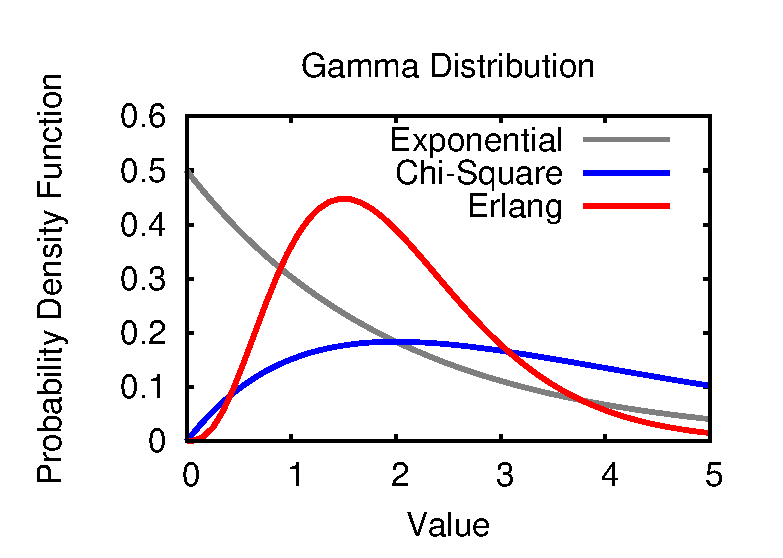
\includegraphics[width=8.5cm]{Figures/8chapter/gamma_pdf}
\end{center}
\caption{Gamma distributions form a two-parameter family of PDFs and, depending on $(\alpha, \lambda)$, they can be employed to model various situations.
The parameters used above are $(1, 0.5)$ for the exponential distribution, $(2, 0.5)$ for the chi-square distribution and $(4, 2)$ for the Erlang distribution;
they are all instances of gamma distributions.}
\label{figure:GammaDistribution}
\end{figure}

\paragraph{The Exponential Distribution:}
When $\alpha = 1$, the gamma distribution simply reduces to the exponential distribution discussed in Section~\ref{section:ExponentialDistribution}.

\paragraph{The Chi-Square Distribution:}
When $\lambda = 1/2$ and $\alpha = k/2$ for some positive integer $k$, the gamma distribution becomes a \emph{chi-square distribution},
\begin{equation*}
f_X (x) = \frac{x^{\frac{k}{2} - 1} e^{-\frac{x}{2}}}{2^{\frac{k}{2}}\Gamma (k/2)} \quad  x > 0.
\end{equation*}
The chi-square distribution is one of the probability distributions most widely used in statistical inference problems.


\paragraph{The Erlang Distribution:}
When $\alpha = m$, a positive integer, the gamma distribution is called an \emph{Erlang distribution}.
This distribution finds application in queueing theory.
Its PDF is given by
\begin{equation*}
f_X (x) = \frac{\lambda (\lambda x)^{m - 1} e^{-\lambda x}}{(m-1)!} \quad  x > 0.
\end{equation*}

An $m$-Erlang random variable can be obtained by summing $m$ independent exponential random variables.
Specifically, let $X_1, X_2, \ldots, X_m$ be independent exponential random variables, each with parameter $\lambda > 0$.
The random variable $S_m$ given by
\begin{equation*}
S_m = \sum_{k=1}^m X_k
\end{equation*}
is an Erlang random variable with parameter $m$ and $\lambda$.

\begin{example}
Suppose that service requests at an Internet are characterized by independent, memoryless inter-arrival periods.
Let $S_m$ be a random variable that denotes the time of the $m$th arrival, then $S_m$ is an Erlang  random variable.
\end{example}


\subsection{The Rayleigh Distribution}

The Rayleigh PDF is given by \index{Rayleigh random variable}
\begin{equation*}
f_X (x) = \frac{x}{\sigma^2} e^{- \frac{x^2}{2 \sigma^2} } \quad x \geq 0 .
\end{equation*}
The \emph{Rayleigh distribution} arises in the context of wireless communications.
Suppose that $Y_1$ and $Y_2$ are two independent normal random variables, then the  magnitude of this random vectors possesses a Rayleigh distribution.
Also, if $X$ is a Rayleigh random variable then $X^2$ has an exponential distribution.

\begin{figure}[ht]
\begin{center}
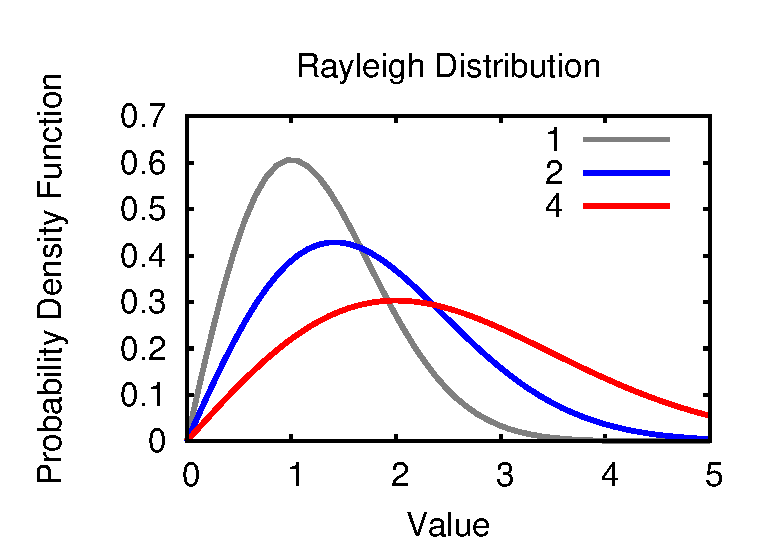
\includegraphics[width=8.5cm]{Figures/8chapter/rayleigh_pdf}
\end{center}
\caption{This figure plots the distributions of Rayleigh random variables for parameters $\sigma^2 \in \{ 1, 2, 4 \}$.}
\end{figure}


\subsection{The Laplace Distribution}
The \emph{Laplace distribution} is sometimes called a double exponential distribution because it can be thought of as an exponential function and its reflection spliced together. \index{Laplace random variable}
The PDF of a Laplacian random variable then becomes
\begin{equation*}
f_X (x) = \frac{1}{2b} e^{- \frac{|x|}{b}} \quad - \infty < x < \infty,
\end{equation*}
where $b$ is a positive constant.
The difference between two independent and identically distributed exponential random variables is governed by a Laplace distribution.

\begin{figure}[ht]
\begin{center}
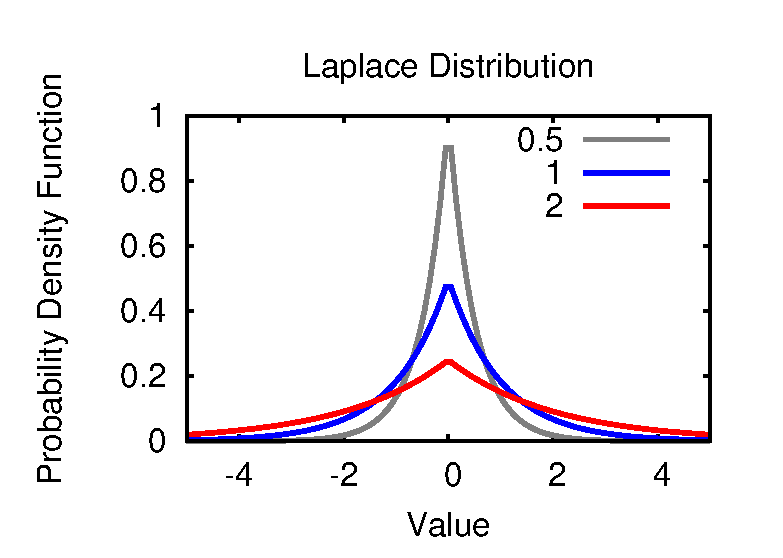
\includegraphics[width=8.5cm]{Figures/8chapter/laplace_pdf}
\end{center}
\caption{The PDF of a Laplace random variable can be constructed using an exponential function and its reflection spliced together.
This figures shows Lapace PDFs for parameters $b \in \{0.5, 1, 2 \}$.}
\end{figure}


\subsection{The Cauchy Distribution}
The \emph{Cauchy distribution} is considered a heavy-tail distribution. \index{Cauchy random variable}
The PDF of a Cauchy random variable is given by
\begin{equation*}
f_X (x) = \frac{ \gamma^2 }{\pi \left( \gamma^2 + x^2 \right)} \quad - \infty < x < \infty.
\end{equation*}
An interesting fact about this distribution is that, although its median is zero, it does not have a mean.
Cauchy random variables are sometimes used in detection theory to model communication systems subject to extreme noise conditions; they also finds applications in physics.
Physicists sometimes refer to this distribution as the \emph{Lorentz distribution}.

\begin{figure}[ht]
\begin{center}
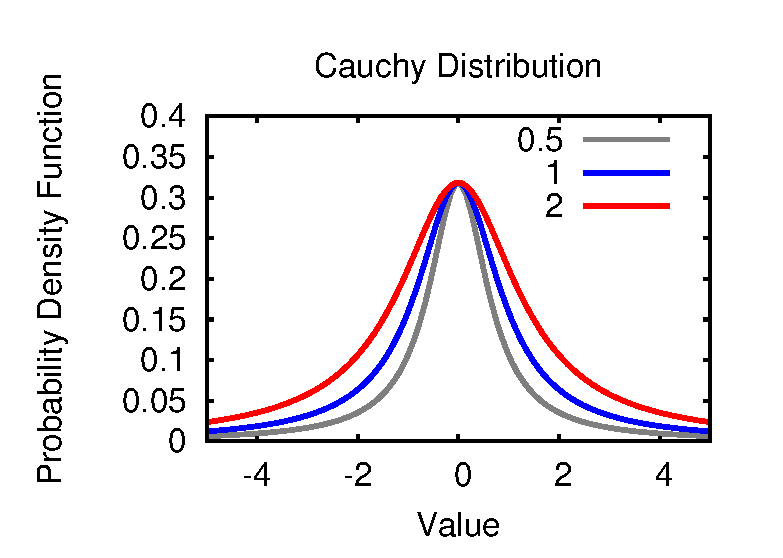
\includegraphics[width=8.5cm]{Figures/8chapter/cauchy_pdf}
\end{center}
\caption{%Cauchy distributions are categorized as heavy-tail distributions because of their very slow decay.
The PDFs of Cauchy random variables are shown above for parameters $\gamma^2 \in \{ 1, 2, 4 \}$.}
\end{figure}


%\chapter{Functions and Derived Distributions}
\index{Functions of Random Variables}

We have already seen that it is possible to form new discrete random variables by applying real-valued functions to existing random variables.
In a similar manner, it is possible to generate a new random variable $Y$ by taking a well-behaved function $g(\cdot)$ of a continuous random variable $X$.
The graphical interpretation of this notion is analog to the discrete case and appears below.

\begin{figure}[ht]
\begin{center}
\begin{psfrags}
\psfrag{S}[l]{Sample Space}
\psfrag{X}[c]{$X$}
\psfrag{Y}[c]{$Y = g(X)$}
\includegraphics[width=9.26cm]{Figures/9Chapter/fcn}
\end{psfrags}
\caption{A function of a random variable is a random variable itself.
In this figure, $Y$ is obtained by applying function $g(\cdot)$ to the value of continuous random variable $X$.}
\end{center}
\end{figure}

Let $X$ be a continuous random variable, and let $g: \RealNumbers \mapsto \RealNumbers$ be an admissible function.
Variable $Y = g(X)$, defined pointwise, is itself random.
The probability that $Y$ falls in a specific set $S$ depends on both the function $g(\cdot)$ and the PDF of $X$,
\begin{equation*}
\Pr (Y \in S) = \Pr (g(X) \in S) 
= \Pr \left( X \in g^{-1}(S) \right).
\end{equation*}
In particular, we can derive the CDF of $Y$ using the formula
\begin{equation} \label{equation:DerivedCDF}
F_Y(y) = \Pr (g(X) \leq y) = \int_{ \{ \xi \in X(\Omega) | g(\xi) \leq y \} } f_X(\xi) d\xi .
\end{equation}

\begin{example}
Let $X$ be a Rayleigh  random variable with parameter $\sigma^2  = 1$, and define $Y = X^2$.
We wish to find the distribution of $Y$.
From \eqref{equation:DerivedCDF}, we can compute the CDF of $Y$.
For $y > 0$, we get
\begin{equation*}
\begin{split}
F_Y(y) &= \Pr (Y \leq y) = \Pr \left( X^2 \leq y \right) \\
&= \Pr (- \sqrt{y} \leq X \leq \sqrt{y})
= \int_0^{\sqrt{y}} \xi e^{- \frac{\xi^2}{2}} d\xi \\
&= \int_0^{y} \frac{1}{2} e^{- \frac{\zeta}{2}} d\zeta
= 1 - e^{-\frac{y}{2}} .
\end{split}
\end{equation*}
We have employed the fact that $X \geq 0$ in determining the boundaries of integration, and we have used the substitution $\zeta = \xi^2$ in computing the integral.
We recognize $F_Y(\cdot)$ as the CDF of an exponential random variable.
This shows that the square of a Rayleigh random variable has an exponential distribution.
\end{example}

The fact that $X$ is a continuous random variable does not provide much insight on the properties of $Y$.
In general, $Y$ could be a continuous random variable, a discrete random variable or neither.
To gain a better understanding of derived distributions, we begin our exposition of functions of continuous random variables by exploring special cases.


\section{Monotone Functions}

A \emph{monotonic function} is a function which preserves a given order.
For instance, $g(\cdot)$ is monotonically increasing if, for all $x_1$ and $x_2$ such that $x_1 \leq x_2$, we get $g(x_1) \leq g(x_2)$.
Likewise, a function $g(\cdot)$ is termed monotonically decreasing provided that $g(x_1) \geq g(x_2)$ whenever $x_1 \leq x_2$.
Monotonic functions of continuous random variable are easy to handle.
For non-decreasing function $g(\cdot)$ of random variable $X$, we have
\begin{equation} \label{equation:MonotoneIncreasingCDF}
\begin{split}
F_Y(y) &= \Pr ( Y \leq y) = \Pr ( g(X) \leq y) \\
&= \Pr \left( X \leq \sup \{ g^{-1} (y) \} \right)
= F_X \left( \sup \{ g^{-1} (y) \} \right) .
\end{split}
\end{equation}
The supremum comes from the fact that multiple values of $x$ may lead to a same value of $y$; that is, the set $g^{-1}(y) = \{ x | g(x) = y \}$ may contain several elements.
These elements all need to be accounted for in our expression, and this is accomplished by selecting the largest one.

\begin{figure}[ht]
\begin{center}
\begin{psfrags}
\psfrag{x}[c]{$g^{-1} = \{ x | g(x) = y \}$}
\psfrag{y}[c]{$y$}
\psfrag{X}[c]{$X$}
\psfrag{Y}[c]{$Y$}
\includegraphics[width=6.5cm]{Figures/9Chapter/MonotoneIncreasing}
\end{psfrags}
\caption{A function of a random variable is a random variable itself.
In this figure, $Y$ is obtained by passing random variable $X$ through a function $g(\cdot)$.}
\end{center}
\end{figure}

\begin{example}
Let $X$ be a continuous random variable uniformly distributed over interal $[0, 1]$.
We wish to characterize the derived distribution of $Y = 2X$.
This can be accomplished as follows; for $y \in [0, 2]$, we have
\begin{equation*}
\begin{split}
F_Y(y) &= \Pr (Y \leq y) = \Pr \left( X \leq \frac{y}{2} \right) \\
&= \int_0^{\frac{y}{2}} dx = \frac{y}{2} .
\end{split}
\end{equation*}
Thus, $Y$ is a uniform random variable with support $[0, 2]$.
By taking derivatives, we obtain the PDF of $Y$ as
\begin{equation*}
f_Y(y) = \begin{cases} \frac{1}{2}, & y \in [0, 2] \\
0, & \text{otherwise}. \end{cases}
\end{equation*}
\end{example}

Alternatively, suppose that $g(\cdot)$ is a \emph{monotone decreasing} function and let $Y = g(X)$.
The CDF of $Y$ is then equal to
\begin{equation} \label{equation:MonotoneDecreasingCDF}
\begin{split}
F_Y(y) &= \Pr (Y \leq y) = \Pr (g(X) \leq y) \\
&= \Pr \left( X \geq \inf \{ g^{-1} (y) \} \right)
= 1 - F_X \left( \inf \{ g^{-1} (y) \} \right) .
\end{split}
\end{equation}
This is very similar to the previous case in that the infimum accounts for the fact that the set $g^{-1} = \{ x | g(x) = y \}$ may contain multiple elements.
Also, note that \eqref{equation:MonotoneDecreasingCDF} relies on the fact that $X$ is a continuous random variable.


\section{Differentiable Functions}

As discussed at the beginning of the chapter, a function of a continuous random variable does not necessarily result in a continuous random variable.
To gain insight about this topic, it is best to first consider the situation where $g(\cdot)$ is a differentiable and strictly increasing function.
Note that, with these two properties, $g(\cdot)$ becomes an invertible function.
It is therefore possible to write $x = g^{-1} (y)$, as the value of $x$ is unambiguous.
In such a case, we can write the CDF of $Y$ as
\begin{equation*}
\begin{split}
F_Y(y) &= \Pr (Y \leq y) = \Pr (g(X) \leq y) \\
&= \Pr \left( X \leq g^{-1}(y) \right)
= F_X \left( g^{-1} (y) \right) .
\end{split}
\end{equation*}
Differentiating this equation with respect to $y$, we obtain the PDF of $Y$
\begin{equation*}
\begin{split}
f_Y (y) &= \frac{d}{dy} F_Y(y)
= \frac{d}{dy} F_X \left( g^{-1} (y) \right) \\
&= f_X \left( g^{-1} (y) \right) \frac{d}{dy} g^{-1} (y)
= f_X \left( g^{-1} (y) \right) \frac{dx}{dy} .
\end{split}
\end{equation*}
With the simple substitution $x = g^{-1} (y)$, we get
\begin{equation*}
f_Y (y) = f_X (x) \frac{dx}{dy}
= \frac{f_X (x)}{g'(x)} .
\end{equation*}
Note that $g'(x)$ is non-zero because $g(\cdot)$ is a strictly increasing function.
From this analysis, we gather that $Y=g(X)$ is a continuous random variable.
More specifically, if $g(\cdot)$ is a differentiable and strictly increasing function, then we can express the PDF of $Y = g(X)$ in terms of the PDF of $X$ and the derivative of $g(\cdot)$.

Similarly, suppose that $g$ is a differentiable and strictly decreasing function.
In this case, the CDF of the random variable $Y = g(X)$ becomes
\begin{equation*}
F_Y(y) = \Pr (g(X) \leq y)
= \Pr \left( X \geq g^{-1}(y) \right)
= 1 - F_X \left( g^{-1} (y) \right) ,
\end{equation*}
and its PDF is given by
\begin{equation*}
\begin{split}
f_Y (y) &= \frac{d}{dy} \left( 1 - F_X \left( g^{-1} (y) \right) \right) \\
&= - f_X \left( g^{-1} (y) \right) \frac{dx}{dy}
= \frac{f_X (x)}{- g'(x)} .
\end{split}
\end{equation*}
Again, we find that $Y = g(X)$ is a continuous random variable and the PDF of $Y$ can be written in therms of $f_X( \cdot)$ and the derivative of $g(\cdot)$.

Combining these two results, we observe that if $g(\cdot)$ is differentiable and strictly monotone, the PDF of $Y$ becomes
\begin{equation} \label{equation:MonotoneFunctionPDF}
f_Y (y) = f_X \left( g^{-1} (y) \right) \left| \frac{dx}{dy} \right|
= \frac{f_X (x)}{\left| g'(x) \right|}
\end{equation}
where $x = g^{-1}(y)$.

\begin{example}
Suppose that $X$ is a Gaussian random variable with PDF
\begin{equation*}
f_X(x) = \frac{1}{\sqrt{2 \pi}} e^{- \frac{x^2}{2}} .
\end{equation*}
We wish to find the PDF of random variable $Y$ where $Y = a X + b$ and $a \neq 0$.

In this example, $g(x) = ax + b$.
The inverse of function of $g$ is then equal to
\begin{equation*}
x = g^{-1} (y) = \frac{y - b}{a} ,
\end{equation*}
and its derivative is given by
\begin{equation*}
\frac{dx}{dy} = \frac{d}{dy} g^{-1}(y) = \frac{1}{a} .
\end{equation*}
The PDF of $Y$ can be computed using \eqref{equation:MonotoneFunctionPDF}, which yields
\begin{equation*}
f_Y(y) = f_X \left( g^{-1} (y) \right) \left| \frac{dx}{dy} \right|
= \frac{1}{\sqrt{2 \pi} |a|} e^{- \frac{(y-b)^2}{2 a^2} }.
\end{equation*}
Thus, an affine function of a Gaussian random variable is also a Gaussian random variable.
\end{example}

Finally, suppose that $g(\cdot)$ is a differentiable function with a finite number of local extrema.
Then, $g(\cdot)$ is piecewise monotonic and we can write the PDF of $Y= g(X)$ as
\begin{equation} \label{equation:FunctionPDF}
f_Y (y) = \sum_{\{ x \in X(\Omega) | g(x) = y\}}
\frac{f_X (x)}{\left| g'(x) \right|} .
\end{equation}
In words, $f_Y (y)$ is obtained by first identifying all the values of $x$ for which $g(x) = y$.
The PDF of $Y$ is then computed explicitly by finding the local contribution of each of these values to $f_Y(y)$ using the methodology developed above.
This is accomplished by applying \eqref{equation:MonotoneFunctionPDF} repetitively to every value of $x$ such that $g(x) = y$.
% This is illustrated in Figure.
It is certainly useful to compare \eqref{equation:FunctionPDF} to its discrete equivalent \eqref{equation:DefinitionFunctionPMF}, which is easier to understand and visualize.

\begin{example}
The distribution of a Rayleigh random variable is given by
\begin{equation*}
f_X (x) = \frac{x}{\sigma^2} e^{- \frac{x^2}{2 \sigma^2} } \quad x \geq 0,
\end{equation*}
where $\sigma > 0$.
Let $Y = X^2$ and find the distribution of random variable $Y$.

Since $Y$ is the square of $X$, we have $g(x) = x^2$.
The PDF of $Y$ is found to be
\begin{equation*}
f_Y(y) = \frac{f_X (x)}{|g'(x)|}
= \frac{1}{\sigma^2} e^{- \frac{x^2}{2 \sigma^2} }
= \frac{1}{2 \sigma^2} e^{- \frac{y}{2 \sigma^2} }
\end{equation*}
where $y \geq 0$.
Random variable $Y$ has an exponential distribution with parameter $2 \sigma^2$.
Note that we do not need to account for the negative square root $x = - \sqrt{y}$ since the Rayleigh random variable has a one-side PDF.
\end{example}


\section{Generating Random Variables}

In engineering, computer simulations are often used as a first step in validating a concept or evaluating design candidates.
Many such projects involve the generation of multiple random variables.
In this section, we explore a methodology that can be employed to generate arbitrary random variable based on a number generator that outputs a random variable uniformly distributed between zero and one.

\subsection{Continuous Random Variables}

For the continuous case, we begin with a simple observation.
Let $X$ be a continuous random variable with PDF $f_X (\cdot)$.
Consider the random variable $Y = F_X(X)$.
Since $F_X (\cdot)$ is differentiable and strictly increasing over the support of $X$, we get
\begin{equation*}
f_Y (y) = \frac{f_X (x)}{| F_X'(x) |}
= \frac{f_X (x)}{| f_X (x) |} = 1
\end{equation*}
where $y \in [0, 1]$ and $x = F_X^{-1} (y)$.
The PDF of $Y$ is zero outside of this interval because $0 \leq F_X (x) \leq 1$.
Thus, using an arbitrary continuous random variable $X$, we can generate a uniform random variable $Y$ with PDF
\begin{equation*}
f_Y(y) = \begin{cases} 1 & y \in [0,1] \\
0 & \text{otherwise} . \end{cases}
\end{equation*}

This provides valuable insight about our original goal.
Suppose that $Y$ is a continuous random variable uniformly distributed over $[0,1]$.
We wish to generate continuous random variable $Z$ with CDF $F_X(\cdot)$.
First, we note that, when $F_X (\cdot)$ is invertible, we have
\begin{equation*}
F_X^{-1} \left( F_X (X) \right) = X .
\end{equation*}
Thus, applying $F_X^{-1} (\cdot)$ to the uniform random variable $Y$ should work.
Define $Z = F_X^{-1} (Y)$, and consider the PDF of $Z$.
Using our previous results, we have
\begin{equation*}
\begin{split}
f_Z (z) = \frac{ f_Y (y) }{ \left| \frac{d F_X^{-1}}{dy} (y) \right| }
= f_Y (y) \frac{d F_X}{dy} (z) = f_X (z)
\end{split}
\end{equation*}
where $y = F_X (z)$.
Hence, this technique can be employed to generate a random variable with PDF $f_X (\cdot)$ from a continuous random variable that is uniformly distributed over $[0,1]$.
More specifically, to create a continuous random variable $X$ with CDF $F_X (\cdot)$, one can apply the function $F_X^{-1} (\cdot)$ to a random variable $Y$ that is uniformly distributed over $[0,1]$.

\begin{example}
Suppose that $Y$ is a continuous random variable uniformly distributed over $[0,1]$.
We wish to create an exponential random variable $X$ with parameter $\lambda$ by taking a function of $Y$.

Random variable $X$ is nonnegative, and its CDF is given by $F_X(x) = 1 - e^{- \lambda x}$ for $x \geq 0$.
The inverse of $F_X (\cdot)$ is given by
\begin{equation*}
F_X^{-1} (y) = - \frac{ \log (1 - y) }{\lambda} .
\end{equation*}
Thus, we can generate the desired random variable $X$ as
\begin{equation*}
X = - \frac{ \log (1 - Y) }{\lambda} .
\end{equation*}
For $x \geq 0$, we have
\begin{equation*}
f_X (x) = \frac{ f_Y (y) }{ \frac{1}{\lambda (1 - y)} }
= \lambda e^{- \lambda x}
\end{equation*}
where we have use the notation $y = 1 - e^{- \lambda x}$.
This is indeed the expected result.
\end{example}


\section{Multiple Continuous Random Variables}

Probability density functions can be extended to the case of multiple continuous random variable.
We denote the \emph{joint probability density function} of random variables $X$ and $Y$ by $f_{X,Y} (\cdot, \cdot)$. \index{Joint Probability Density Function}
In general, $f_{X,Y} (\cdot, \cdot)$ is a nonnegative function such that
\begin{equation*}
\int_{-\infty}^{\infty} \int_{-\infty}^{\infty}
f_{X, Y} (\xi, \zeta) d\zeta d\xi = 1.
\end{equation*}
Furthermore, for a measurable set $S$, the probability that $(X,Y) \in S$ can be computed through the integral
\begin{equation*}
\begin{split}
\Pr ((X,Y) \in S)
&= \int_{-\infty}^{\infty} \int_{-\infty}^{\infty}
\mathrm{1}_{S}(\xi, \zeta) f_{X, Y} (\xi, \zeta) d\zeta d\xi \\
&= \int \int_{S}
f_{X, Y} (\xi, \zeta) d\zeta d\xi .
\end{split}
\end{equation*}
If $S$ is the rectangular set
\begin{equation*}
S = \left\{ (x,y) \in X(\Omega) \times Y(\Omega) \big| a \leq x \leq b, c \leq y \leq d \right\} ,
\end{equation*}
then the probability that $(X,Y) \in S$ becomes the typical integral
\begin{equation*}
\Pr ((X,Y) \in S)
= \Pr (a \leq X \leq b, c \leq Y \leq d)
= \int_{a}^{b} \int_{c}^{d}
f_{X, Y} (\xi, \zeta) d\zeta d\xi .
\end{equation*}

\begin{example}
Suppose that the random pair $(X, Y)$ is uniformly distributed over the unit circle.
Then, the joint PDF $f_{X,Y} (\cdot, \cdot)$ is given by
\begin{equation*}
f_{X,Y} (x, y) = \begin{cases} \frac{1}{\pi} & x^2 + y^2 \leq 1 \\
0 & \text{otherwise} . \end{cases}
\end{equation*}
We wish to find the probability that the point $(X, Y)$ lies inside the circle of radius $1/2$.

Let $S = \{ (x, y) \in X(\Omega) \times Y(\Omega) | x^2 + y^2 \leq 0.5 \}$.
The probability that $(X, Y)$ lies in $S$ is given by
\begin{equation*}
\Pr ((X,Y) \in S)
= \int_{-\infty}^{\infty} \int_{-\infty}^{\infty}
\mathbf{1}_{S}(\xi, \zeta) \frac{1}{\pi} d\xi d\zeta
= \frac{1}{4} .
\end{equation*}
Thus, the probability that $(X,Y)$ lies in the circle of radius half is one fourth.
\end{example}

It is also possible to define the \emph{joint cumulative distribution function} of a pair of random variables, \index{Joint cumulative distribution function}
\begin{equation*}
F_{X,Y} (x,y) = \Pr (X \leq x, Y \leq y) .
\end{equation*}
For continuous random variables, the joint CDF of $X$ and $Y$ can derived from their joint PDF,
\begin{equation*}
F_{X,Y} (x,y) = \int_{-\infty}^x \int_{-\infty}^y f_{X,Y} (\xi,\zeta) d\zeta d\xi .
\end{equation*}
Calculus asserts that the following is also true,
\begin{equation*}
f_{X,Y} (x,y) = \frac{\partial^2 F_{X,Y}}{\partial x \partial y} (x,y) .
\end{equation*}


\subsection{Conditional Distribution}

It is possible to derive the PDF of a random variable condition on a certain event, or on another random variable.
Let $X$ and $Y$ be two random variable associated with the same experiment.
The \emph{conditional probability distribution function} of $Y$ given $X = x$, denoted by $f_{Y|X}$, is defined by
\begin{equation} \label{equation:ContinuousConditonalPDF}
f_{Y|X} (y|x) = \frac{f_{X,Y} (x,y)}{f_X(x)},
\end{equation}
provided that $f_X(x) \neq 0$.
We emphasize that there is a strong similarity between the definition of the conditional PDF and PMF.
For a fixed value $X = x$, the conditional PDF $f_{Y|X} (y|x)$ is a legitimate PDF since it is nonnegative and it integrates to one.

\begin{example}
Consider a random experiment where an outcome $(\omega_1, \omega_2)$ is selected at random from the unit circle.
Let $X = \omega_1$ and $Y = \omega_2$.
We wish to compute the conditional PDF of $Y$ given that $X = \sqrt{3}{2}$.
We apply the definition of the conditional PDF, with
\begin{equation*}
\begin{split}
f_{Y|X} \left( y \Big| \frac{1}{2} \right)
= \frac{f_{X,Y} \left( \frac{1}{2}, y \right)}
{\int_{-\frac{\sqrt{3}}{2}}^{\frac{\sqrt{3}}{2}}
f_{X,Y} \left( \frac{1}{2} , \zeta \right) d \zeta }
= \begin{cases} \frac{1}{\sqrt{3}} & |y| \leq \frac{\sqrt{3}}{2} \\
0 & \text{otherwise} . \end{cases}
\end{split}
\end{equation*}
\end{example}

Let $\{ Y \in S \}$ be an event such that $\Pr (Y \in S) > 0$.
The conditional PDF of $Y$ given $\{ Y \in S \}$ is defined by
\begin{equation*}
f_{Y|S} (y)
= \left\{ \begin{array}{cc} \frac{ f_Y(y) }{\Pr (Y \in S)}, & y \in S \\
0, & \text{otherwise}. \end{array} \right.
\end{equation*}
This PDF can be used to compute the conditional probability of specific events given $Y \in S$.
Let $T$ be a measurable set, then
\begin{equation*}
\begin{split}
\Pr ( Y \in T | Y \in S)
&= \frac{ \Pr ( Y \in T \cap Y \in S) }{ \Pr ( Y \in S) } \\
&= \frac{ \int_{Y \cap T} f_Y(y) dy }{ \Pr ( Y \in S) } \\
&= \int_{T} f_{Y|S} (y) dy .
\end{split}
\end{equation*}

%\begin{example}
%\end{example}


\subsection{Independence}

Two continuous random variables $X$ and $Y$ are mutually \emph{independent} if their joint CDF is the product of their respective CDFs, \index{independence}
\begin{equation*}
F_{X,Y} (x,y) = F_X (x) F_Y(y)
\end{equation*}
for any $x \in X(\Omega)$ and $y \in Y(\Omega)$.
We emphasize that this necessarily implies that the joint PDF is the product of the individual PDFs as well,
\begin{equation*}
f_{X,Y} (x,y) = \frac{\partial^2 F_{X,Y}}{\partial x \partial y} (x, y)
= \frac{d F_X}{dx} (x) \frac{d F_Y}{dy} (y)
= f_X (x) f_Y (y)
\end{equation*}
for any $x \in X(\Omega)$ and $y \in Y(\Omega)$.

From \eqref{equation:ContinuousConditonalPDF}, we gather that the conditional PDF of $Y$ given $X=x$ is equal to the marginal PDF of $Y$ whenever $X$ and $Y$ are independent
\begin{equation*}
f_{Y|X} (y|x) = \frac{f_{X,Y} (x, y)}{f_X(x)}
= \frac{f_X (x) f_Y (y)}{f_X(x)} = f_Y (y),
\end{equation*}
provided that $f_X(x) \neq 0$.
Furthermore, if $X$ and $Y$ are independent random variables, then the two events $\{ X \in S \}$ and $\{ Y \in T \}$ are independent
\begin{equation*}
\begin{split}
&\Pr (X \in S, Y \in T) = \int_S \int_T f_{X,Y} (x,y) dy dx \\
&= \int_S f_X (x) dx \int_T f_Y (y) dy
= \Pr (X \in S) \Pr (Y \in T).
\end{split}
\end{equation*}

\begin{example}
Consider a random experiment where an outcome $(\omega_1, \omega_2)$ is selected at random from the unit square.
Let $X = \omega_1$, $Y = \omega_2$ and $Z = \omega_1 + \omega_2$.
We wish to show that $X$ and $Y$ are independent, and that $X$ and $Z$ are not independent.

We begin by computing the joint CDF of $X$ and $Y$.
For $x,y \in [0,1]$, we have
\begin{equation*}
F_{X,Y}(x,y) = \int_0^{x} \int_0^{y} d\zeta d\xi
= x y = F_X(x) F_Y(y) .
\end{equation*}
More generally, if $x, y \in \mathbb{R}^2$, we get
\begin{equation*}
\begin{split}
F_{X,Y}(x,y)
&= \int_{-\infty}^{x} \int_{-\infty}^{y}
\mathbf{1}_{[0,1]^2} (\xi, \zeta) d\zeta d\xi \\
&= \int_{-\infty}^{x} \mathbf{1}_{[0,1]} (\xi) d \xi
\int_{-\infty}^{y} \mathbf{1}_{[0,1]} (\zeta) d\zeta
= F_X(x) F_Y(y) .
\end{split}
\end{equation*}
Thus, we gather that $X$ and $Y$ are independent.

Next, we show that $X$ and $Z$ are not independent.
First, we note that $F_Z (1) = \frac{1}{2}$ and $F_X (1/2) = 1/2$.
Consider the joint CDF of $X$ and $Z$ evaluated at $(1/2, 1)$,
\begin{equation*}
\begin{split}
F_{X,Z} \left( \frac{1}{2} ,1 \right)
&= \int_{0}^{\frac{1}{2}} \int_{0}^{1-\xi} d\zeta d\xi
= \int_{0}^{\frac{1}{2}} (1 - \xi) d\xi \\
%&= \frac{1}{2} - \frac{1}{8} \\
&= \frac{3}{8}
\neq F_X \left( \frac{1}{2} \right) F_Z(1) .
\end{split}
\end{equation*}
Thus, $X$ and $Z$ are clearly not independent.
\end{example}



%\chapter{Expectations and Bounds}

The concept of expectation, has now been introduced in the context of discrete and continuous random variables.
We know from our previous discussion that expectations provide an effective way to summarize the information contained in the distribution of a random variable.
As we will see shortly, expectations are also very valuable in establishing bounds on probabilities.

\iffalse

\section{Expectations Revisited}

The definition of an expectation associated with a continuous random variable is very similar to its discrete counterpart;
the weighted sum is simply replaced by a weighted integral.
For a continuous random variable $X$ with PDF $f_X(\cdot)$, the \emph{expectation} of $g(X)$ is defined by \index{Expectation}
\begin{equation*}
\Expect [g(X)]
= \int_{\RealNumbers} g(\xi) f_X (\xi) d\xi .
\end{equation*}
In particular, the \emph{mean} of $X$ is equal to \index{Mean}
\begin{equation*}
\Expect [X]
= \int_{\RealNumbers} \xi f_X (\xi) d\xi
\end{equation*}
and its \emph{variance} becomes \index{Variance}
\begin{equation*}
\Var [X] = \Expect \left[ (X - \Expect[X])^2 \right]
= \int_{\RealNumbers} (\xi - \Expect[X])^2 f_X (\xi) d\xi .
\end{equation*}
As before, the variance of random variable $X$ can also be computed using $\Var [X] = \Expect \left[ X^2 \right] - \left( E[X] \right)^2$.

\begin{example}
We wish to calculate the mean and variance of a Gaussian random variable with parameters $m$ and $\sigma^2$.
By definition, the PDF of this random variable can be written as
\begin{equation*}
f_X (\xi) = \frac{1}{\sqrt{2 \pi} \sigma} e^{-\frac{(\xi - m)^2}{2\sigma^2}}
\quad \xi \in \RealNumbers .
\end{equation*}
The mean of $X$ can be obtained through direct integration, with a change of variables,
\begin{equation*}
\begin{split}
\Expect [X]
&= \frac{1}{\sqrt{2 \pi} \sigma} \int_{- \infty}^{\infty} \xi e^{-\frac{(\xi-m)^2}{2\sigma^2}} d\xi \\
&= \frac{\sigma}{\sqrt{2 \pi}} \int_{- \infty}^{\infty}
\left( \zeta+\frac{m}{\sigma} \right) e^{-\frac{\zeta^2}{2}} d\zeta \\
&= \frac{\sigma}{\sqrt{2 \pi}} \int_{- \infty}^{\infty}
\zeta e^{-\frac{\zeta^2}{2}} d\zeta
+ \frac{\sigma}{\sqrt{2 \pi}} \int_{- \infty}^{\infty}
\frac{m}{\sigma} e^{-\frac{\zeta^2}{2}} d\zeta
= m.
\end{split}
\end{equation*}
In finding a solution, we have leveraged the facts that $\zeta e^{-\frac{\zeta^2}{2}}$ is an absolutely integrable, odd function.
We also took advantage of the normalization condition which ensures that a Gaussian PDF integrates to one.
To derive the variance, we again use the normalization condition.
For a Gaussian PDF, this property implies that
\begin{equation*}
\int_{-\infty}^{\infty} e^{- \frac{(\xi-m)^2}{2 \sigma^2}} d\xi
= \sqrt{2 \pi} \sigma .
\end{equation*}
Differentiating both sides of this equation with respect to $\sigma$, we get
\begin{equation*}
\int_{-\infty}^{\infty} \frac{(\xi-m)^2}{\sigma^3}
e^{- \frac{(\xi-m)^2}{2 \sigma^2}} d\xi
= \sqrt{2 \pi} .
\end{equation*}
Rearranging the terms yields
\begin{equation*}
\int_{-\infty}^{\infty} \frac{(\xi-m)^2}{\sqrt{2 \pi} \sigma}
e^{- \frac{(\xi-m)^2}{2 \sigma^2}} d\xi
= \sigma^2 .
\end{equation*}
Hence, $\Var [X] = \Expect \left[ (X-m)^2 \right] = \sigma^2$.
Of course, the variance can also be obtained by more conventional methods.
\end{example}


\begin{example}
Suppose that $R$ is a Rayleigh random variable with parameter $\sigma^2$.
We wish to compute its mean and variance.

Recall that $R$ is a nonnegative random variable with PDF
\begin{equation*}
f_R (r) = \frac{r}{\sigma^2} e^{- \frac{r^2}{2 \sigma^2} } \quad r \geq 0 .
\end{equation*}
Using this distribution, we get
\begin{equation*}
\begin{split}
\Expect [R] &= \int_0^{\infty} \xi f_R(\xi) d\xi
= \int_0^{\infty} \frac{\xi^2}{\sigma^2} e^{- \frac{\xi^2}{2 \sigma^2}} d\xi \\
&= \left. - \xi e^{- \frac{\xi^2}{2 \sigma^2}} \right|_0^{\infty}
+ \int_0^{\infty} e^{- \frac{\xi^2}{2 \sigma^2}} d\xi \\
&= \sqrt{ 2 \pi } \sigma
\int_0^{\infty} \frac{1}{\sqrt{2 \pi} \sigma} e^{- \frac{\zeta^2}{2 \sigma^2}} d\zeta
= \frac{\sqrt{2 \pi} \sigma}{2} .
\end{split}
\end{equation*}
Integration by parts is key in solving this expectation.
Also, notice the judicious use of the fact that the integral of a standard normal random variable over $[0, \infty)$ must be equal to $1/2$.
We compute the second moment of $R$ below,
\begin{equation*}
\begin{split}
\Expect \left[ R^2 \right] &= \int_0^{\infty} \xi^2 f_R(\xi) d\xi
= \int_0^{\infty} \frac{\xi^3}{\sigma^2} e^{- \frac{\xi^2}{2 \sigma^2}} d\xi \\
&= \left. - \xi^2 e^{- \frac{\xi^2}{2 \sigma^2}} \right|_0^{\infty}
+ \int_0^{\infty} 2 \xi e^{- \frac{\xi^2}{2 \sigma^2}} d\xi \\
&= \left. - 2 \sigma^2 e^{- \frac{\xi^2}{2 \sigma^2}} \right|_0^{\infty}
= 2 \sigma^2 .
\end{split}
\end{equation*}
The variance of $R$ is therefore equal to
\begin{equation*}
\Var [R] = \frac{(4 - \pi)}{2} \sigma^2 .
\end{equation*}
Typically, $\sigma^2$ is employed to denote the variance of a random variable.
It may be confusing at first to have a random variable $R$ described in terms of parameter $\sigma^2$ whose variance is equal to $(4 - \pi) \sigma^2/2$.
This situation is an artifact of the following relation.
A Rayleigh random variable $R$ can be generated through the expression $R = \sqrt{X^2 + Y^2}$, where $X$ and $Y$ are independent zero-mean Gaussian variables with variance $\sigma^2$.
Thus, the parameter $\sigma^2$ in $f_R (\cdot)$ is a tribute to this popular construction, not a representation of its actual variance.
\end{example}

For nonnegative random variable $X$, an alternative way to compute $\Expect [X]$ is described in Proposition~\ref{proposition:MeanAlternative}. \index{Expectation}

\begin{proposition} \label{proposition:MeanAlternative}
Suppose that $X$ is a nonnegative random variable with finite mean, then
\begin{equation*}
\Expect [X] = \int_0^{\infty} \Pr (X > x) dx .
\end{equation*}
\end{proposition}
\begin{proof}
We offer a proof for the special case where $X$ is a continuous random variable, although the result remains true in general,
\begin{equation*}
\begin{split}
\int_0^{\infty} \Pr (X > x) dx
&= \int_0^{\infty} \int_x^{\infty} f_X(\xi) d\xi dx \\
&= \int_0^{\infty} \int_0^{\xi} f_X(\xi) dx d\xi \\
&= \int_0^{\infty} \xi f_X(\xi) d\xi
= \Expect [X] .
\end{split}
\end{equation*}
Interchanging the order of integration is justified because $X$ is assumed to have finite mean.
\end{proof}

\begin{example}
A player throws darts at a circular target hung on a wall.
The dartboard has unit radius, and the position of every dart is distributed uniformly over the target.
We wish to compute the expected distance from each dart to the center of the dartboard.

Let $R$ denote the distance from a dart to the center of the target.
For $0 \leq r \leq 1$, the probability that $R$ exceeds $r$ is given by
\begin{equation*}
\Pr (R > r) = 1 - \Pr (R \leq r) = 1 - \frac{\pi r^2}{\pi} = 1 - r^2 .
\end{equation*}
Then, by Proposition~\ref{proposition:MeanAlternative}, the expected value of $R$ is equal to
\begin{equation*}
\Expect [R] = \int_0^1 \left( 1 - r^2 \right) dr
= \left.  \left( r - \frac{r^3}{3} \right) \right|_0^1
= 1 - \frac{1}{3} = \frac{2}{3} .
\end{equation*}
Notice how we were able to compute the answer without deriving an explicit expression for $f_R (\cdot)$.
\end{example}

\fi

\section{Moment Generating Functions}

The \emph{moment generating function} of a random variable $X$ is defined by
\begin{equation*}
M_X (s) = \Expect \left[ e^{s X} \right] .
\end{equation*}
For continuous random variables, the moment generating function becomes
\begin{equation*}
M_X (s) = \int_{-\infty}^{\infty} f_X (\xi) e^{s \xi} d\xi .
\end{equation*}
The experienced reader will quickly recognize the definition of $M_X(s)$ as a variant of the \emph{Laplace Transform}, a widely used linear operator.
The moment generating function gets its name from the following property.
Suppose that $M_X(s)$ exists within an open interval around $s = 0$, then the $n$th moment of $X$ is given by
\begin{equation*}
\begin{split}
\frac{d^n}{ds^n} M_X (s) \Big|_{s=0}
&= \frac{d^n}{ds^n} \Expect \left[ e^{s X} \right] \Big|_{s=0}
= \Expect \left[ \frac{d^n}{ds^n} e^{s X} \right] \bigg|_{s=0} \\
&= \Expect \left[ X^n e^{s X} \right] \Big|_{s=0}
= \Expect [X^n] .
\end{split}
\end{equation*}
In words, if we differentiate $M_X(s)$ a total of $n$ times and then evaluate the resulting function at zero, we obtain the $n$th moment of $X$.
In particular, we have $\frac{d M_X}{ds}(0) = \Expect [X]$ and $\frac{d^2 M_X}{ds^2}(0) = \Expect [X^2]$.

\begin{example}[Exponential Random Variable]
Let $X$ be an exponential random variable with parameter $\lambda$.
The moment-generating function of $X$ is given by
\begin{equation*}
M_X (s) = \int_0^{\infty} \lambda e^{-\lambda \xi} e^{s\xi} d\xi
= \int_0^{\infty} \lambda e^{-(\lambda-s) \xi} d\xi
= \frac{\lambda}{\lambda - s} .
\end{equation*}
The mean of $X$ is
\begin{equation*}
\Expect [X] = \frac{d M_X }{ds} (0)
= \left. \frac{\lambda}{(\lambda - s)^2} \right|_{s=0}
= \frac{1}{\lambda} ;
\end{equation*}
more generally, the $n$th moment of $X$ can be computed as
\begin{equation*}
\Expect [X^n] = \frac{d^n M_X }{ds^n} (0)
= \left. \frac{n! \lambda}{(\lambda - s)^{n+1}} \right|_{s=0}
= \frac{n!}{\lambda^n} .
\end{equation*}
Incidentally, we can deduce from these results that the variance of $X$ is $1/\lambda^2$.
\end{example}

The definition of the moment generating function applies to discrete random variables as well.
In fact, for integer-valued random variables, the moment generating function and the ordinary generating function are related through the equation \index{Ordinary generating function} \index{Moment generating function}
\begin{equation*}
M_X (s) = \sum_{k \in X(\Omega)} e^{sk} p_X(k) = G_X (e^s) .
\end{equation*}

\begin{example}[Discrete Uniform Random Variable]
Suppose $U$ is a discrete uniform random variable taking value in $U(\Omega) = \{ 1, 2, \ldots, n \}$.
Then, $p_U(k) = 1/n$ for $1 \leq k \leq n$ and
\begin{equation*}
M_U(s) = \sum_{k = 1}^n \frac{1}{n} e^{sk}
= \frac{1}{n} \sum_{k = 1}^n e^{sk}
= \frac {e^s (e^{ns} - 1)} {n (e^s - 1)} .
\end{equation*}
The moment generating function provides an alternate and somewhat intricate way to compute the mean of $U$,
\begin{equation*}
\begin{split}
\Expect [U] &= \frac{d M_U}{ds} (0)
= \lim_{s \rightarrow 0}
\frac{n e^{(n+2)s} - (n+1) e^{(n+1)s} + e^s}{n \left( e^s - 1 \right)^2} \\
&= \lim_{s \rightarrow 0}
\frac{n(n+2) e^{(n+1)s} - (n+1)^2 e^{ns} + 1}{2n \left( e^s - 1 \right)} \\
&= \lim_{s \rightarrow 0}
\frac{n(n+1)(n+2)n e^{(n+1)s} - n (n+1)^2 e^{ns}}{2n e^s}
= \frac {n + 1}{2} .
\end{split}
\end{equation*}
Notice the double application of \emph{l'H\^{o}pital's rule} to evaluate the derivative of $M_U(s)$ at zero.
This may be deemed a more contrived method to derive the expected value of a discrete uniform random variables, but it does not rely on prior knowledge of special sums.
Through similar steps, one can derive the second moment of $U$, which is equal to
\begin{equation*}
\Expect \left[ U^2 \right] = \frac{(n+1)(2n+1)}{6} .
\end{equation*}
From these two results, we can show that the variance of $U$ is $(n^2 - 1)/12$.
\end{example}

The simple form of the moment generating function of a standard normal random variable points to its importance in many situations.
The exponential function is analytic and possesses many representations.

\begin{example}[Gaussian Random Variable]
Let $X$ be a standard normal random variable whose PDF is given by
\begin{equation*}
f_X (\xi) = \frac{1}{\sqrt{2 \pi}} e^{- \frac{\xi^2}{2}}.
\end{equation*}
The moment generating function of $X$ is equal to
\begin{equation*}
\begin{split}
M_X (s) &= \Expect \left[ e^{sX} \right]
= \int_{- \infty}^{\infty} \frac{1}{\sqrt{2 \pi}} e^{- \frac{\xi^2}{2}} e^{s\xi} d\xi \\
&= \int_{- \infty}^{\infty} \frac{1}{\sqrt{2 \pi}} e^{- \frac{\xi^2 + 2 s \xi}{2}} d\xi
= e^{\frac{s^2}{2}} \int_{- \infty}^{\infty}
\frac{1}{\sqrt{2 \pi}} e^{- \frac{\xi^2 - 2 s \xi + s^2}{2}} d\xi \\
&= e^{\frac{s^2}{2}} \int_{- \infty}^{\infty}
\frac{1}{\sqrt{2 \pi}} e^{- \frac{(\xi - s)^2}{2}} d\xi
= e^{\frac{s^2}{2}} .
\end{split}
\end{equation*}
The last equality follows from the normalization condition and the fact that the integrand is a Gaussian PDF.
\end{example}

Let $M_X(s)$ be the moment generating function associated with a random variable $X$, and consider the random variable $Y = aX + b$ where $a$ and $b$ are constant.
The moment generating function of $Y$ can be obtained as follows,
\begin{equation*}
M_Y (s) = \Expect \left[ e^{s X} \right]
= \Expect \left[ e^{s (aX + b)} \right]
= e^{sb} \Expect \left[ e^{saX} \right]
= e^{sb} M_X (as) .
\end{equation*}
Thus, if $Y$ is an affine function of $X$ then $M_Y (s) = e^{sb} M_X (as)$.

\begin{example}
We can use this property to identify the moment generating function of a Gaussian random variable with parameters $m$ and $\sigma^2$.
Recall that an affine function of a Gaussian random variable is also Gaussian.
Let $Y = \sigma X + m$, then the moment generating function of $Y$ becomes
\begin{equation*}
M_Y (s) = \Expect \left[ e^{sY} \right]
= \Expect \left[ e^{s(\sigma X + m)} \right]
= e^{sm} \Expect \left[ e^{s\sigma X} \right]
= e^{sm + \frac{s^2 \sigma^2}{2} } .
\end{equation*}
From this moment generating function, we get
\begin{align*}
\Expect [Y] &= \frac{d M_Y}{ds} (0)
= \left. \left[ \left(m + s \sigma^2 \right)
e^{sm + \frac{s^2 \sigma^2}{2} } \right] \right|_{s=0} = m \\
\begin{split}
\Expect \left[ Y^2 \right] &= \frac{d^2 M_Y}{ds^2} (0)
= \left.  \left[ \sigma^2 e^{sm + \frac{s^2 \sigma^2}{2} }
+ \left(m + s \sigma^2 \right)^2  e^{sm + \frac{s^2 \sigma^2}{2} } \right]
\right|_{s=0} \\
&= \sigma^2 + m^2 .
\end{split}
\end{align*}
The mean of $Y$ is $m$ and its variance is equal to $\sigma^2$, as anticipated.
\end{example}


\section{Important Inequalities}

There are many situations for which computing the exact value of a probability is impossible or impractical.
In such cases, it may be acceptable to provide bounds on the value of an elusive probability.
The expectation is most important in finding pertinent bounds.

As we will see, many upper bounds rely on the concept of dominating functions.
Suppose that $g(x)$ and $h(x)$ are two nonnegative function such that $g(x) \leq h(x)$ for all $x \in \RealNumbers$.
Then, for any continuous random variable $X$, the following inequality holds
\begin{equation*}
\begin{split}
\Expect [g(X)] &= \int_{-\infty}^{\infty} g(x) f_X(x) dx \\
&\leq \int_{-\infty}^{\infty} h(x) f_X (x) dx
= \Expect [h(X)] .
\end{split}
\end{equation*}
This is illustrated in Figure~\ref{figure:DominatingFcn}.
In words, the weighted integral of $g(\cdot)$ is dominated by the weighted integral of $h(\cdot)$, where $f_X (\cdot)$ acts as the weighting function.
This notion is instrumental in understanding bounding techniques.
\begin{figure}[thb]
\begin{center}
\begin{psfrags}
\psfrag{Y}[c]{$\RealNumbers$}
\psfrag{X}[c]{$\RealNumbers$}
\psfrag{h}[c]{$h(x)$}
\psfrag{g}[c]{$g(x)$}
\includegraphics[width=6.5cm]{Figures/10Chapter/DominatingFcn}
\end{psfrags}
\caption{If $g(x)$ and $h(x)$ are two nonnegative functions such that $g(x) \leq h(x)$ for all $x \in \RealNumbers$, then $\Expect [g (X)]$ is less than or equal to $\Expect [h(X)]$.}
\label{figure:DominatingFcn}
\end{center}
\end{figure}


\subsection{The Markov Inequality}

We begin our exposition of classical upper bounds with a result known as the \emph{Markov inequality}. \index{Markov inequality}
Recall that, for admissible set $S \subset \RealNumbers$, we have
\begin{equation*}
\Pr (X \in S) = \Expect \left[ \IndicatorFcn_S (X) \right] .
\end{equation*}
Thus, to obtain a bound on $\Pr (X \in S)$, it suffices to find a function that dominates $\IndicatorFcn_S (\cdot)$ and for which we can compute the expectation.

Suppose that we wish to bound $\Pr (X \geq a)$ where $X$ is a nonnegative random variable.
In this case, we can select $S = [a, \infty)$ and function $h(x) = x/a$.
For any $x \geq 0$, we have $h(x) \geq \IndicatorFcn_S(x)$, as illustrated in Figure~\ref{figure:MarkovInequality}.
It follows that
\begin{equation*}
\Pr (X \geq a) = \Expect \left[ \IndicatorFcn_S(X) \right] \leq \frac{\Expect [X]}{a} .
\end{equation*}

\begin{figure}[thb]
\begin{center}
\begin{psfrags}
\psfrag{Y}[c]{$\RealNumbers$}
\psfrag{X}[c]{$\RealNumbers$}
\psfrag{h}[l]{$h(x) = \frac{x}{a}$}
\psfrag{g}[l]{$g(x) = \IndicatorFcn_S (x)$}
\psfrag{a}[c]{$a$}
\includegraphics[width=6.5cm]{Figures/10Chapter/Markov}
\end{psfrags}
\caption{Suppose that we wish to find a bound for $\Pr (X \leq a)$.
We define set $S = [a, \infty)$ and function $g(x) = \IndicatorFcn_S (x)$.
Using dominating function $h(x) = x/a$, we conclude that $\Pr(X \geq a) \leq a^{-1} \Expect [X]$ for any nonnegative random variable $X$.}
\label{figure:MarkovInequality}
\end{center}
\end{figure}


\subsection{The Chebyshev Inequality}

The \emph{Chebyshev inequality} provides an extension to this methodology to various dominating functions. \index{Chebyshev inequality}
This yields a number of bounds that become useful in a myriad of contexts.

\begin{proposition}[Chebyshev Inequality]
Suppose $h (\cdot)$ is a nonnegative function and let $S$ be an admissible set.
We denote the infimum of $h (\cdot)$ over $S$ by
\begin{equation*}
i_S = \inf_{ x \in S } h (x) .
\end{equation*}
The Chebyshev inequality asserts that
\begin{equation} \label{equation:ChebyshevInequality}
i_S \Pr (X \in S)
\leq \Expect [ h(X) ]
\end{equation}
where $X$ is an arbitrary random variable.
\end{proposition}
\begin{proof}
This is a remarkably powerful result and it can be shown in a few steps.
The definition of $i_S$ and the fact that $h (\cdot)$ is nonnegative imply that
\begin{equation*}
i_S \IndicatorFcn_S (x) \leq h(x) \IndicatorFcn_S (x) \leq h(x)
\end{equation*}
for any $x \in \RealNumbers$.
Moreover, for any such $x$ and distribution $f_X(\cdot)$, we can write $i_S \IndicatorFcn_S (x) f_X(x) \leq h(x) f(x)$, which in turn yields
\begin{equation*}
\begin{split}
i_S \Pr (X \in S) &= \Expect \left[ i_s \IndicatorFcn_S (X) \right]
= \int_{\RealNumbers} i_S \IndicatorFcn_S (\xi) f_X(\xi) d\xi \\
&\leq \int_{\RealNumbers} h (\xi) f_X(\xi) d\xi
= \Expect [ h(X) ] .
\end{split}
\end{equation*}
When $i_S > 0$, this provides the upper bound $\Pr (X \in S) \leq i_S^{-1} \Expect [h (X)]$.
\end{proof}

Although the proof assumes a continuous random variable, we emphasize that the Chebyshev inequality applies to both discrete and continuous random variables alike.
The interested reader can rework the proof using the discrete setting and a generic PMF.
We provide special instances of the Chebyshev inequality below.

\begin{example}
Consider the nonnegative function $h(x) = x^2$ and let $S = \{ x | x^2 \geq b^2 \}$ where $b$ is a positive constant.
We wish to find a bound on the probability that $|X|$ exceeds $b$.
Using the Chebyshev inequality, we have $i_S = \inf_{x \in S} x^2 = b^2$ and, consequently, we get
\begin{equation*}
b^2 \Pr (X \in S) \leq \Expect \left[ X^2 \right] .
\end{equation*}
Constant $b$ being a positive real number, we can rewrite this equation as
\begin{equation*}
\Pr (|X| \geq b) = \Pr (X \in S) \leq \frac{\Expect \left[ X^2 \right]}{b^2} .
\end{equation*}
\end{example}

\begin{example}[The Cantelli Inequality]
Suppose that $X$ is a random variable with mean $m$ and variance $\sigma^2$.
We wish to show that
\begin{equation*}
\Pr ( X - m \geq a ) \leq \frac{\sigma^2}{a^2 + \sigma^2},
\end{equation*}
where $a \geq 0$.

This equation is slightly more involved and requires a small optimization in addition to the Chebyshev inequality.
Define $Y = X - m$ and note that, by construction, we have $\Expect [Y] = 0$.
Consider the probability $\Pr (Y \geq a)$ where $a > 0$, and let $S = \{ y | y \geq a \}$.
Also, define the nonnegative function $h(y) = (y + b)^2$, where $b > 0$.
Following the steps of the Chebyshev inequality, we write the infimum of $h(y)$ over $S$ as
\begin{equation*}
i_S = \inf_{y \in S} (y + b)^2 = (a + b)^2 .
\end{equation*}
Then, applying the Chebyshev inequality, we obtain
\begin{equation} \label{equation:CantelliProof}
\Pr (Y \geq a) \leq \frac{ \Expect \left[ (Y + b)^2 \right] }{(a + b)^2}
= \frac{ \sigma^2 + b^2 }{ (a + b)^2 } .
\end{equation}
This inequality holds for any $b > 0$.
To produce a better upper bound, we minimize the right-hand side of \eqref{equation:CantelliProof} over all possible values of $b$.
Differentiating this expression and setting the derivative equal to zero yields
\begin{equation*}
\frac{ 2 b }{(a + b)^2 } = \frac{ 2 \left( \sigma^2 + b^2 \right) }{(a + b)^3}
\end{equation*}
or, equivalently, $b = \sigma^2 / a$.
A second derivative test reveals that this is indeed a minimum.
Collecting these results, we obtain
\begin{equation*}
\Pr (Y \geq a) \leq \frac{ \sigma^2 + b^2 }{ (a + b)^2 }
%= \frac{ \sigma^2 + \sigma^4/a^2 }{ (a + \sigma^2/a)^2 }
%= \frac{ \sigma^2 (a^2 + \sigma^2) }{ (a^2 + \sigma^2)^2 }
= \frac{ \sigma^2 }{ a^2 + \sigma^2 } .
\end{equation*}
Substituting $Y = X - m$ leads to the desired result.
\end{example}

In some circumstances, a Chebyshev inequality can be tight.

\begin{example}
Let $a$ and $b$ be two constants such that $0 < b \leq a$.
Consider the function $h(x) = x^2$ along with the set $S = \{ x | x^2 \geq a^2 \}$.
Furthermore, let $X$ be a discrete random variable with PMF
\begin{equation*}
p_X (x) = \left\{ \begin{array}{ll} 1 - \frac{b^2}{a^2}, & x = 0 \\
\frac{b^2}{a^2}, & x = a \\
0, & \text{otherwise.} \end{array} \right.
\end{equation*}
For this random variable, we have $\Pr (X \in S) = b^2/a^2$.
By inspection, we also gather that the second moment of $X$ is equal to $\Expect \left[ X^2 \right] = b^2$.
Applying the Chebyshev inequality, we get $i_S = \inf_{x \in S} h(x) = a^2$ and therefore
\begin{equation*}
\Pr (X \in S) \leq i_S^{-1} \Expect \left[ h(X) \right]
= \frac{b^2}{a^2} .
\end{equation*}
Thus, in this particular example, the inequality is met with equality.
\end{example}


\subsection{The Chernoff Bound}

The \emph{Chernoff bound} is yet another upper bound that can be constructed from the Chebyshev inequality. \index{Chernoff bound}
Still, because of its central role in many application domains, it deserves its own section.
Suppose that we want to find a bound on the probability $\Pr (X \geq a)$.
We can apply the Chebyshev inequality using the nonnegative function $h(x) = e^{sx}$, where $s > 0$.
For this specific construction, $S = [a, \infty)$ and
\begin{equation*}
i_S = \inf_{x \in S} e^{sx} = e^{sa} .
\end{equation*}
It follows that
\begin{equation*}
\Pr (X \geq a) \leq e^{-sa} \Expect[ e^{sX} ] = e^{-sa} M_X(s) .
\end{equation*}
Because this inequality holds for any $s > 0$, we can optimize the upper bound over all possible values of $s$, thereby picking the best one,
\begin{equation} \label{equation:ChernoffBound}
\Pr (X \geq a) \leq \inf_{s > 0} e^{-sa} M_X(s) .
\end{equation}
This inequality is called the Chernoff bound.
It is sometimes expressed in terms of the log-moment generating function $\Lambda (s) = \log M_X (s)$.
In this latter case, \eqref{equation:ChernoffBound} translates into
\begin{equation} \label{equation:LogChernoffBound}
\log \Pr (X \geq a) \leq - \sup_{s > 0} \left\{ sa - \Lambda (s) \right\} .
\end{equation}
The right-hand side of \eqref{equation:LogChernoffBound} is called the \emph{Legendre transformation} of $\Lambda (s)$. \index{Legendre transformation}
Figure~\ref{figure:ChernoffBound} plots $e^{s(x-a)}$ for various values of $s > 0$.
It should be noted that all these functions dominate $\IndicatorFcn_{[a, \infty)}(x)$, and therefore they each provide a different bound on $\Pr (X \geq a)$.
It is natural to select the function that provides the best bound.
Yet, in general, this optimal $e^{s(x-a)}$ may depend on the distribution of $X$ and the value of $a$, which explains why \eqref{equation:ChernoffBound} involves a search over all possible values of $s$.

\begin{figure}[ht]
\begin{center}
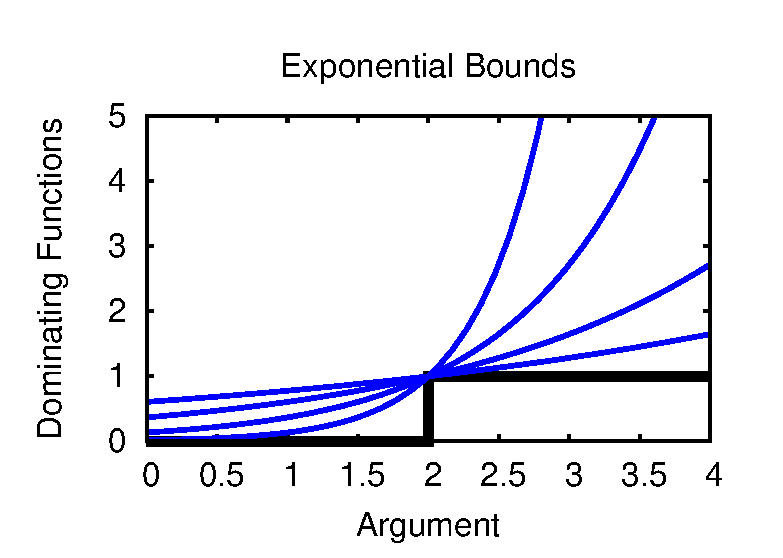
\includegraphics[width=8.5cm]{Figures/10chapter/chernoff_bound}
\end{center}
\caption{This figure illustrates how exponential functions can be employed to provide bounds on $\Pr (X > a)$.
Optimizing over all admissible exponential functions, $e^{s(x-a)}$ where $s > 0$, leads to the celebrated Chernoff bound.}
\label{figure:ChernoffBound}
\end{figure}


\subsection{Jensen's Inequality}

Some inequalities can be derived based on the properties of a single function.
The \emph{Jensen inequality} is one such example. \index{Jensen inequality}
Suppose that function $g(\cdot)$ is convex and twice differentiable, with
\begin{equation*}
\frac{d^2 g}{dx^2} (x) \geq 0
\end{equation*}
for all $x \in \RealNumbers$.
From the fundamental theorem of calculus, we have
\begin{equation*}
g(x) = g(a) + \int_a^x \frac{dg}{dx} (\xi) d\xi .
\end{equation*}
Futhermore, because the second derivative of $g(\cdot)$ is a non-negative function, we gather that $\frac{dg}{dx} (\cdot)$ is a monotone increasing function.
As such, for any value of $a$, we have
\begin{equation*}
\begin{split}
g(x) &= g(a) + \int_a^x \frac{dg}{dx} (\xi) d\xi \\
&\geq g(a) + \int_a^x \frac{dg}{dx} (a) d\xi
= g(a) + (x-a) \frac{dg}{dx} (a) .
\end{split}
\end{equation*}
For random variable $X$, we then have
\begin{equation*}
g(X) \geq g(a) + (X-a) \frac{dg}{dx} (a) .
\end{equation*}
Choosing $a = \Expect [X]$ and taking expectations on both sides, we obtain
\begin{equation*}
\Expect [g(X)] \geq g(\Expect [X])
+ (\Expect [X]-\Expect [X]) \frac{dg}{dx} (\Expect [X])
= g(\Expect [X]) .
\end{equation*}
That is, $\Expect [g(X)] \geq g(\Expect [X])$, provided that these two expectations exist.
The Jensen inequality actually holds for convex functions that are not twice differentiable, but the proof is much harder in the general setting.


\section*{Further Reading}

\begin{small}
\begin{enumerate}
\item Ross, S., \emph{A First Course in Probability}, 7th edition, Pearson Prentice Hall, 2006: Sections~5.2, 7.7, 8.2.
\item Bertsekas, D. P., and Tsitsiklis, J. N., \emph{Introduction to Probability}, Athena Scientific, 2002: Section~3.1, 4.1, 7.1.
\item Gubner, J. A., \emph{Probability and Random Processes for Electrical and Computer Engineers}, Cambridge, 2006: Sections~4.2--4.3.
\item Miller, S. L., and Childers, D. G., \emph{Probability and Random Processes with Applications to Signal Processing and Communications}, 2004: Section~5.2.
\end{enumerate}
\end{small}


%\chapter{Multiple Continuous Random Variables}

Being versed at dealing with multiple random variables is an essential part of statistics, engineering and science.
This is equally true for models based on discrete and continuous random variables.
In this chapter, we focus on the latter and expand our exposition of continuous random variables to random vectors.
Again, our initial survey of this topic revolves around conditional distributions and pairs of random variables.
More complex scenarios will be considered in the later parts of the chapter.


\section{Joint Cumulative Distributions}

Let $X$ and $Y$ be two random variables associated with a same experiment.
The \emph{joint cumulative distribution function} of $X$ and $Y$ is defined by \index{Joint cumulative distribution function}
\begin{equation*}
F_{X,Y} (x, y) = \Pr (X \leq x, Y \leq y) \quad x, y \in \RealNumbers .
\end{equation*}
Keeping in mind that $X$ and $Y$ are real-valued functions acting on a same sample space, we can also write
\begin{equation*}
F_{X,Y} (x, y) = \Pr \left( \{ \omega \in \Omega | X(\omega) \leq x, Y(\omega) \leq y \} \right) .
\end{equation*}
From this characterization, we can identify a few properties of the joint CDF;
\begin{equation*}
\begin{split}
\lim_{y \uparrow \infty} F_{X,Y} (x, y)
&= \lim_{y \uparrow \infty} \Pr \left( \{ \omega \in \Omega | X(\omega) \leq x, Y(\omega) \leq y \} \right) \\
&= \Pr \left( \{ \omega \in \Omega | X(\omega) \leq x, Y(\omega) \in \RealNumbers \} \right) \\
&= \Pr \left( \{ \omega \in \Omega | X(\omega) \leq x \} \right)
= F_X (x) .
\end{split}
\end{equation*}
Similarly, we have $\lim_{x \uparrow \infty} F_{X,Y} (x,y) = F_Y (y)$.
Taking limits in the other direction, we get
\begin{equation*}
\lim_{x \downarrow -\infty} F_{X,Y} (x,y) 
= \lim_{y \downarrow -\infty} F_{X,Y} (x,y) = 0 .
\end{equation*}

When the function $F_{X,Y} (\cdot, \cdot)$ is totally differentiable, it is possible to define the \emph{joint probability density function} of $X$ and $Y$, \index{Joint probability density function}
\begin{equation} \label{equation:JointPDF}
f_{X,Y} (x,y) = \frac{\partial^2 F_{X,Y}}{\partial x \partial y} (x,y)
= \frac{\partial^2 F_{X,Y}}{\partial y \partial x} (x,y) \quad x,y \in  \RealNumbers .
\end{equation}
Hereafter, we refer to a pair of random variables as continuous if the corresponding joint PDF exists and is defined unambiguously through \eqref{equation:JointPDF}.
When this is the case, standard calculus asserts that the following equation holds,
\begin{equation*}
F_{X,Y} (x,y) = \int_{-\infty}^x \int_{-\infty}^y f_{X,Y} (u,v) dv du .
\end{equation*}
From its definition, we note that $f_{X,Y} (\cdot, \cdot)$ is a nonnegative function which integrates to one,
\begin{equation*}
\iint\limits_{\RealNumbers^2}
f_{X, Y} (u, v) dv du = 1.
\end{equation*}
Furthermore, for any admissible set $S \subset \RealNumbers^2$, the probability that $(X,Y) \in S$ can be evaluated through the integral formula
\begin{equation} \label{equation:ProbabilityJointPDF}
\begin{split}
\Pr ((X,Y) \in S)
&= \iint\limits_{\RealNumbers^2}
\IndicatorFcn_{S} (x, y) f_{X, Y} (x, y) dy dx \\
&= \iint\limits_{S}
f_{X, Y} (x, y) dy dx .
\end{split}
\end{equation}
In particular, if $S$ is the cartesian product of two intervals, 
\begin{equation*}
S = \left\{ (x,y) \in \RealNumbers^2 \big| a \leq x \leq b, c \leq y \leq d \right\} ,
\end{equation*}
then the probability that $(X,Y) \in S$ reduces to the typical integral form
\begin{equation*}
\Pr ((X,Y) \in S)
= \Pr (a \leq X \leq b, c \leq Y \leq d)
= \int_{a}^{b} \int_{c}^{d}
f_{X, Y} (x, y) dy dx .
\end{equation*}

\begin{example}
Suppose that the random pair $(X, Y)$ is uniformly distributed over the unit circle.
We can express the joint PDF $f_{X,Y} (\cdot, \cdot)$ as
\begin{equation*}
f_{X,Y} (x, y) = \begin{cases} \frac{1}{\pi} & x^2 + y^2 \leq 1 \\
0 & \text{otherwise} . \end{cases}
\end{equation*}
We wish to find the probability that the point $(X, Y)$ lies inside a circle of radius $1/2$.

Let $S = \{ (x, y) \in \RealNumbers^2 | x^2 + y^2 \leq 0.5 \}$.
The probability that $(X, Y)$ belongs to $S$ is given by
\begin{equation*}
\Pr ((X,Y) \in S)
= \iint\limits_{\RealNumbers^2}
\frac{\mathbf{1}_{S}(x, y)}{\pi} dx dy
= \frac{1}{4} .
\end{equation*}
Thus, the probability that $(X,Y)$ is contained within a circle of radius half is one fourth.
\end{example}

\begin{example}
Let $X$ and $Y$ be two independent zero-mean Gaussian random variables, each with variance $\sigma^2$.
For $(x, y) \in \RealNumbers^2$, their joint PDF is given by
\begin{equation*}
f_{X,Y} (x,y) = \frac{1}{2 \pi \sigma^2} e^{- \frac{x^2 + y^2}{2 \sigma^2} } .
\end{equation*}
We wish to find the probability that $(X,Y)$ falls within a circle of radius $r$ centered at the origin.

We can compute this probability using integral formula \eqref{equation:ProbabilityJointPDF} applied to this particular problem.
Let $R = \sqrt{X^2 + Y^2}$ and assume $r > 0$, then
\begin{equation*}
\begin{split}
\Pr (R \leq r) &= \iint\limits_{R \leq r} f_{X,Y} (x,y) dx dy
= \iint\limits_{R \leq r} \frac{1}{2 \pi \sigma^2}
e^{- \frac{ x^2 + y^2 }{2 \sigma^2} } (x,y) dx dy \\
&= \int_0^r \int_0^{2\pi} \frac{1}{2 \pi \sigma^2}
e^{- \frac{ r^2 }{2 \sigma^2} } r d\theta dr
= 1 - e^{- \frac{ r^2 }{2 \sigma^2} } .
\end{split}
\end{equation*}
The probability that $(X, Y)$ is contained within a circle of radius $r$ is $1 - e^{- \frac{ r^2 }{2 \sigma^2} }$.
Recognizing that $R$ is a continuous random variable, we can write its PDF as
\begin{equation*}
f_R (r) = \frac{r}{\sigma^2} e^{- \frac{r^2}{2 \sigma^2} } \quad r \geq 0 .
\end{equation*}
From this equation, we gather That $R$ possesses a Rayleigh distribution with parameter $\sigma^2$.
\end{example}


\section{Conditional Probability Distributions}

Given non-vanishing event $A$, we can write the conditional CDF of random variable $X$ as
\begin{equation*}
F_{X|A} (x) = \Pr (X \leq x | A)
= \frac{ \Pr ( \{ X \leq x \} \cap A ) }{\Pr(A)} \quad x \in \RealNumbers .
\end{equation*}
Note that event $A$ can be defined in terms of variables $X$ and $Y$.
For instance, we may use $A = \{ Y \leq X \}$ as our condition.
Under suitable conditions, it is equally straightforward to specify the conditional PDF of $X$ given $A$,
\begin{equation*}
f_{X|A} (x) = \frac{d F_{X|A}}{dx} (x) \quad x \in \RealNumbers .
\end{equation*}

\begin{example}
Let $X$ and $Y$ be continuous random variables with joint PDF
\begin{equation*}
f_{X,Y} (x,y) = \lambda^2 e^{-\lambda (x + y)} \quad x,y \geq 0 .
\end{equation*}
We wish to compute the conditional PDF of $X$ given $A = \{ Y \leq X \}$.
To solve this problem, we first compute the probability of the event $\{ X \leq x \} \cap A$,
\begin{equation*}
\begin{split}
\Pr ( \{ X \leq x \} \cap A )
&= \int_0^x \int_0^{u} f_{X,Y} (u, v) dv du
= \int_0^x \int_0^{u} \lambda^2 e^{-\lambda (u + v)} dv du \\
&= \int_0^x \lambda e^{- \lambda u} \left( 1 - e^{- \lambda u} \right) du
= \frac{ \left( 1 - e^{-\lambda x} \right)^2 }{2} .
\end{split}
\end{equation*}
By symmetry, we gather that $\Pr(A) = 1/2$ and, as such,
\begin{equation*}
f_{X | A} (x) = 2 \lambda e^{-\lambda x} \left( 1 - e^{-\lambda x} \right)
\quad x \geq 0 .
\end{equation*}
\end{example}

One case of special interest is the situation where event $A$ is defined in terms of the random variable $X$ itself.
In particular, consider the PDF of $X$ conditioned on the fact that $X$ belongs to an interval $I$.
Then, $A = \{ X \in I \}$ and the conditional CDF of $X$ becomes
\begin{equation*}
\begin{split}
F_{X|A} (x) &= \Pr (X \leq x | X \in I) \\
&= \frac{ \Pr \left( \{ X \leq x \} \cap \{ X \in I \} \right) }{\Pr(X \in I)} \\
&= \frac{ \Pr \left( X \in (-\infty, x] \cap I \right) }{\Pr(X \in I)} .
\end{split}
\end{equation*}
Differentiating with respect to $x$, we obtain the conditional PDF of $X$,
\begin{equation*}
f_{X|A} (x) = \frac{ f_X (x) }{ \Pr (X \in I) } 
\end{equation*}
for any $x \in I$.
In words, the conditional PDF of $X$ becomes a scaled version of $f_X(\cdot)$ whenever $x \in I$, and it is equal to zero otherwise.
Essentially, this is equivalent to re-normalizing the PDF of $X$ over interval $I$, accounting for the partial information given by $X \in I$.

%\begin{example}
%\end{example}

\subsection{Conditioning on Values}

Suppose that $X$ and $Y$ form a pair of random variables with joint PDF $f_{X,Y} (\cdot, \cdot)$.
With great care, it is possible and desirable to define the conditional PDF of $X$, conditioned on $Y = y$. \index{Conditional probability density function}
Special attention must be given to this situation because the event $\{ Y = y \}$ has probability zero whenever $Y$ is a continuous random variable.
Still, when $X$ and $Y$ are jointly continuous and for any $y \in \RealNumbers$ such that $f_Y (y) > 0$, we can defined the conditional PDF of $X$ given $Y = y$ as
\begin{equation} \label{equation:ConditionalPDF}
f_{X|Y} (x|y) = \frac{ f_{X,Y} (x,y) }{ f_Y (y) } .
\end{equation}
Intuitively, this definition is motivated by the following property.
For small $\Delta_x$ and $\Delta_y$, we can write
\begin{equation*}
\begin{split}
&\Pr (x \leq X \leq x + \Delta_x | y \leq Y \leq y + \Delta_y) \\
&= \frac{\Pr (x \leq X \leq x + \Delta_x, y \leq Y \leq y + \Delta_y)}
{\Pr (y \leq Y \leq y + \Delta_y)} \\
&\approx \frac{f_{X,Y} (x, y) \Delta_x \Delta_y} {f_Y (y) \Delta_y}
= \frac{f_{X,Y} (x, y)}{f_Y (y)} \Delta_x .
\end{split}
\end{equation*}
Thus, loosely speaking, $f_{X|Y} (x|y) \Delta_x$ represents the probability that $X$ lies close to $x$, given that $Y$ is near $y$.

Using this definition, it is possible to compute the probabilities of events associated with $X$ conditioned on a specific value of random variable $Y$,
\begin{equation*}
\Pr (X \in S | Y = y) = \int_S f_{X|Y} (x|y) dx .
\end{equation*}
A word of caution is in order.
The technical difficulty that surfaces when conditioning on $\{ Y = y \}$ stems from the fact that $\Pr (Y = y) = 0$.
Remember that, in general, the notion of conditional probability is only defined for non-vanishing conditions.
Although we were able to circumvent this issue, care must be taken when dealing with the conditional PDF of the form \eqref{equation:ConditionalPDF}, as it only provides valuable insight when the random variables $(X, Y)$ are jointly continuous.

\begin{example}
Consider the experiment where an outcome $(\omega_1, \omega_2)$ is selected at random from the unit circle.
Let $X = \omega_1$ and $Y = \omega_2$.
We wish to compute the conditional PDF of $X$ given that $Y = 0.5$.

First, we compute the marginal PDF of $Y$ evaluated at $Y = 0.5$,
\begin{equation*}
f_Y (0.5) = \int_{\RealNumbers} f_{X,Y} (x, 0.5) dx
= \int_{-\frac{\sqrt{3}}{2}}^{\frac{\sqrt{3}}{2}} \frac{1}{\pi} dx
= \frac{\sqrt{3}}{\pi} .
\end{equation*}
We then apply definition \eqref{equation:ConditionalPDF} to obtain the desired conditional PDF of $X$,
\begin{equation*}
\begin{split}
f_{X|Y} ( x | 0.5 ) &= \frac{f_{X,Y} (x, 0.5)}{f_{Y} ( 0.5 ) }
= \frac{\pi}{\sqrt{3}} f_{X,Y} (x, 0.5) \\
&= \begin{cases} \frac{1}{\sqrt{3}} & |x| \leq \frac{\sqrt{3}}{2} \\
0 & \text{otherwise} . \end{cases}
\end{split}
\end{equation*}
\end{example}

%\begin{example}
%\end{example}

\subsection{Conditional Expectation}

The conditional expectation of a function $g(Y)$ is simply the integral of $g(Y)$ weighted by the proper conditional PDF,
\begin{align*}
E[g(Y) | X = x] &= \int_{\RealNumbers} g(y) f_{Y|X} (y|x) dy \\
E[g(Y) | S] &= \int_{\RealNumbers} g(y) f_{Y|S} (y) dy .
\end{align*}
Note again that the function
\begin{equation*}
h(x) = \Expect [Y | X=x]
\end{equation*}
defines a random variable since the conditional expectation of $Y$ may vary as a function of $X$.
After all, a conditional expectation is itself a random variable.

\begin{example}
An analog communication system transmits a random signal over a noisy channel.
The transmit signal $X$ and the additive noise $N$ are both standard Gaussian random variables, and they are independent.
The signal received at the destination is equal to
\begin{equation*}
Y = X + N .
\end{equation*}
We wish to estimate the value of $X$ conditioned on $Y = y$.

For this problem, the joint PDF of $X$ and $Y$ is
\begin{equation*}
f_{X,Y} (x,y) = \frac{1}{2 \pi}
\exp \left( - \frac{2 x^2 - 2 xy + y^2}{2}  \right)
\end{equation*}
and the conditional distribution of $X$ given $Y$ becomes
\begin{equation*}
\begin{split}
f_{X|Y} (x|y) &= \frac{f_{X,Y} (x,y)}{f_{Y} (y)}
= \frac{ \frac{1}{2 \pi} \exp \left( - \frac{2 x^2 - 2 xy + y^2}{2}  \right) }
{ \frac{1}{2 \sqrt{\pi}} \exp \left( - \frac{y^2}{4}  \right) } \\
&=\frac{1}{\sqrt{\pi}}
\exp \left( - \frac{4 x^2 - 4 xy + y^2}{4}  \right) .
\end{split}
\end{equation*}
By inspection, we recognize that this conditional PDF is a Gaussian distribution with parameters $m = y/2$ and $\sigma^2 = 1/2$.
A widespread algorithm employed to perform the desired task is called the minimum mean square error (MMSE) estimator.
In the present case, the MMSE estimator reduces to the conditional expectation of $X$ given $Y = y$, which is
\begin{equation*}
\Expect [X | Y = y] = \int_{\RealNumbers} x f_{X,Y}(x|y) dx
= \frac{y}{2} .
\end{equation*}
\end{example}


\subsection{Derived Distributions}

Suppose $X_1$ and $X_2$ are jointly continuous random variables.
Furthermore, let $Y_1 = g_1 (X_1, X_2)$ and $Y_2 = g_2 (X_1, X_2)$, where $g_1 (\cdot, \cdot)$ and $g_2 (\cdot, \cdot)$ are real-valued functions.
Under certain conditions, the pair of random variables $(Y_1, Y_2)$ will also be continuous.
Deriving the joint PDF of $(Y_1, Y_2)$ can get convoluted, a task we forgo.
It requires the skillful application of vector calculus.
Nevertheless, we examine the case where a simple expression for $f_{Y_1, Y_2} (\cdot, \cdot)$ exists.

Consider the scenario where the functions $g_1 (\cdot, \cdot)$ and $g_2 (\cdot, \cdot)$ are totally differentiable, with Jacobian determinant
\begin{equation*}
\begin{split}
&|J(x_1, x_2)| = \operatorname{det} \begin{bmatrix}
\frac{\partial g_1}{\partial x_1} (x_1, x_2) &
\frac{\partial g_1}{\partial x_2} (x_1, x_2) \\
\frac{\partial g_2}{\partial x_1} (x_1, x_2) &
\frac{\partial g_2}{\partial x_2} (x_1, x_2)
\end{bmatrix} \\
&= \frac{\partial g_1}{\partial x_1} (x_1, x_2)
\frac{\partial g_2}{\partial x_2} (x_1, x_2)
- \frac{\partial g_1}{\partial x_2} (x_1, x_2)
\frac{\partial g_2}{\partial x_1} (x_1, x_2)
\neq 0 .
\end{split}
\end{equation*}
Also, assume that the system of equations
\begin{align*}
g_1 (x_1, x_2) &= y_1 \\
g_2 (x_1, x_2) &= y_2
\end{align*}
has a unique solution.
We express this solution using $x_1 = h_1 (y_1, y_2)$ and $x_2 = h_2 (y_1, y_2)$.
Then, the random variables $(Y_1, Y_2)$ are jointly continuous with joint PDF
\begin{equation} \label{equation:DerivedJointPDF}
f_{Y_1, Y_2} (y_1, y_2) =
\frac{f_{X_1, X_2} (x_1, x_2)}{ | J(x_1, x_2) |}
\end{equation}
where $x_1 = h_1 (y_1, y_2)$ and $x_2 = h_2 (y_1, y_2)$.
Note the close resemblance between this equation and the derived distribution of \eqref{equation:MonotoneFunctionPDF}.
Looking back at Chapter~\ref{chapter:DerivedDistributions} offers an idea of what proving this result entails.
It also hints at how this equation can be modified to accommodate non-unique mappings.

\begin{example}
An important application of \eqref{equation:DerivedJointPDF} pertains to the properties of Gaussian vectors.
Suppose that $X_1$ and $X_2$ are jointly continuous random variables, and let
\begin{equation*}
\mathbf{X} = \begin{bmatrix} X_1 \\ X_2 \end{bmatrix} .
\end{equation*}
Define the mean of $\mathbf{X}$ by
\begin{equation*}
\mathbf{m} = \Expect [\mathbf{X}] 
= \begin{bmatrix} \Expect[ X_1 ] \\ \Expect[ X_2 ] \end{bmatrix} .
\end{equation*}
and its covariance by
\begin{equation*}
\begin{split}
\Sigma &= \Expect \left[ \left( \mathbf{X} - \mathbf{m} \right)
\left(\mathbf{X} - \mathbf{m} \right)^{\mathrm{T}} \right] \\
&= \begin{bmatrix} \Expect \left[ (X_1 - m_1)^2 \right] &
\Expect[ (X_1 - m_1) (X_2 - m_2) ]  \\
\Expect[ (X_2 - m_2) (X_1 - m_1) ] &
\Expect \left[ (X_2 - m_2)^2 \right] \end{bmatrix} .
\end{split}
\end{equation*}
Random variables $X_1$ and $X_2$ are said to be jointly Gaussian provided that their joint PDF is of the form
\begin{equation*}
f_{X_1, X_2} (x_1, x_2) = \frac{1}{2 \pi |\Sigma|^{\frac{1}{2}}}
\exp \left( - \frac{1}{2} \left( \mathbf{x} - \mathbf{m} \right)^{\mathrm{T}} \Sigma^{-1} \left( \mathbf{x} - \mathbf{m} \right) \right) .
\end{equation*}
Assume that the random variables $Y_1$ and $Y_2$ are generated through the matrix equation
\begin{equation*}
\mathbf{Y} = \begin{bmatrix} Y_1 \\ Y_2 \end{bmatrix}
= A \mathbf{X} + \mathbf{b} ,
\end{equation*}
where $A$ is a $2 \times 2$ invertible matrix and $\mathbf{b}$ is a constant vector.
In this case, $\mathbf{X} = A^{-1} \left( \mathbf{Y} - \mathbf{b} \right)$ and the corresponding Jacobian determinant is
\begin{equation*}
J(x_1, x_2)
= \operatorname{det}
\begin{bmatrix} a_{11} & a_{12} \\ a_{21} & a_{22} \end{bmatrix}
= | A | .
\end{equation*}
Applying \eqref{equation:DerivedJointPDF}, we gather that the joint PDF of $(Y_1, Y_2)$ is expressed as
\begin{equation*}
\begin{split}
&f_{Y_1, Y_2} (y_1, y_2)
%= \frac{ f_{X_1, X_2} (x_1, x_2) }{ |A| }
= \frac{1}{2 \pi |\Sigma|^{\frac{1}{2}} |A|}
\exp \left( - \frac{1}{2}
\left( \mathbf{x} - \mathbf{m} \right)^{\mathrm{T}} \Sigma^{-1} \left( \mathbf{x} - \mathbf{m} \right) \right) \\
&= \frac{1}{2 \pi |A \Sigma A^{\mathrm{T}}|^{\frac{1}{2}}}
\exp \left( - \frac{1}{2}
\left( A^{-1} \left( \mathbf{y} - \mathbf{b} \right) - \mathbf{m} \right)^{\mathrm{T}}
\Sigma^{-1}
\left( A^{-1} \left( \mathbf{y} - \mathbf{b} \right) - \mathbf{m} \right) \right) \\
&= \frac{1}{2 \pi |A \Sigma A^{\mathrm{T}}|^{\frac{1}{2}}}
\exp \left( - \frac{1}{2}
\left( \mathbf{y} - \mathbf{b} - A \mathbf{m} \right)^{\mathrm{T}}
\left( A \Sigma A^{\mathrm{T}} \right)^{-1}
\left( \mathbf{y} - \mathbf{b} - A \mathbf{m} \right) \right) .
\end{split}
\end{equation*}
Looking at this equation, we conclude that random variables $Y_1$ and $Y_2$ are also jointly Gaussian, as their joint PDF possesses the proper form.
It should come as no surprise that the mean of $\mathbf{Y}$ is
$\Expect \left[ \mathbf{Y} \right] = A \mathbf{m} + \mathbf{b}$
and its covariance matrix is equal to
\begin{equation*}
\Expect \left[ \left( \mathbf{Y} - \Expect \left[ \mathbf{Y} \right] \right)
\left( \mathbf{Y} - \Expect \left[ \mathbf{Y} \right] \right)^{\mathrm{T}} \right]
= A \Sigma A^{\mathrm{T}} .
\end{equation*}
In other words, a non-trivial affine transformation of a two-dimensional Gaussian vector yields another Gaussian vector.
This admirable property generalizes to higher dimensions.
Indeed, if $\mathbf{Y} = A \mathbf{X} + \mathbf{b}$ where $A$ is an $n \times n$ invertible matrix and $\mathbf{X}$ is a Gaussian random vector, then $\mathbf{Y}$ remains a Gaussian random vector.
Furthermore, to obtain the derived distribution of the latter vector, it suffices to compute its mean and covariance, and substitute the resulting parameters in the general form of the Gaussian PDF.
Collectively, the features of joint Gaussian random vectors underly many contemporary successes of engineering.
\end{example}


\section{Independence}

Two random variables $X$ and $Y$ are mutually \emph{independent} if their joint CDF is the product of their respective CDFs, \index{Independence}
\begin{equation*}
F_{X,Y} (x,y) = F_X (x) F_Y(y)
\end{equation*}
for $x, y \in \RealNumbers$.
For jointly continuous random variables, this definition necessarily implies that the joint PDF $f_{X,Y}(\cdot, \cdot)$ is the product of their marginal PDFs,
\begin{equation*}
f_{X,Y} (x,y) = \frac{\partial^2 F_{X,Y}}{\partial x \partial y} (x, y)
= \frac{d F_X}{dx} (x) \frac{d F_Y}{dy} (y)
= f_X (x) f_Y (y)
\end{equation*}
for $x, y \in \RealNumbers$.
Furthermore, we gather from \eqref{equation:ConditionalPDF} that the conditional PDF of $Y$ given $X=x$ is equal to the marginal PDF of $Y$ whenever $X$ and $Y$ are independent,
\begin{equation*}
f_{Y|X} (y|x) = \frac{f_{X,Y} (x, y)}{f_X(x)}
= \frac{f_X (x) f_Y (y)}{f_X(x)} = f_Y (y)
\end{equation*}
provided of course that $f_X(x) \neq 0$.
Additionally, if $X$ and $Y$ are independent random variables, then the two events $\{ X \in S \}$ and $\{ Y \in T \}$ are also independent,
\begin{equation*}
\begin{split}
\Pr (X \in S, Y \in T) &= \int_S \int_T f_{X,Y} (x,y) dy dx \\
&= \int_S f_X (x) dx \int_T f_Y (y) dy \\
&= \Pr (X \in S) \Pr (Y \in T).
\end{split}
\end{equation*}

\begin{example}
Consider a random experiment where an outcome $(\omega_1, \omega_2)$ is selected at random from the unit square.
Let $X = \omega_1$, $Y = \omega_2$ and $W = \omega_1 + \omega_2$.
We wish to show that $X$ and $Y$ are independent, but that $X$ and $W$ are not independent.

We begin by computing the joint CDF of $X$ and $Y$.
For $x,y \in [0,1]$, we have
\begin{equation*}
F_{X,Y}(x,y) = \int_0^{x} \int_0^{y} dv du
= x y = F_X(x) F_Y(y) .
\end{equation*}
More generally, if $x, y \in \RealNumbers^2$, we get
\begin{equation*}
\begin{split}
F_{X,Y}(x,y)
&= \int_{-\infty}^{x} \int_{-\infty}^{y}
\mathbf{1}_{[0,1]^2} (u, v) dv du \\
&= \int_{-\infty}^{x} \mathbf{1}_{[0,1]} (u) du
\int_{-\infty}^{y} \mathbf{1}_{[0,1]} (v) dv
= F_X(x) F_Y(y) .
\end{split}
\end{equation*}
Thus, we gather that $X$ and $Y$ are independent.

Next, we show that $X$ and $W$ are not independent.
Note that $F_W (1) = 0.5$ and $F_X (0.5) = 0.5$.
Consider the joint CDF of $X$ and $W$ evaluated at $(0.5, 1)$,
\begin{equation*}
\begin{split}
F_{X,W} (0.5, 1)
&= \int_{0}^{\frac{1}{2}} \int_{0}^{1-x} dw dx
= \int_{0}^{\frac{1}{2}} (1 - x) dx \\
%&= \frac{1}{2} - \frac{1}{8} \\
&= \frac{3}{8}
\neq F_X (0.5) F_W(1) .
\end{split}
\end{equation*}
Clearly, random variables $X$ and $W$ are not independent.
\end{example}


\subsection{Sums of Continuous Random Variables}

As mentioned before, sums of independent random variables are frequently encountered in engineering.
We therefore turn to the question of determining the distribution of a sum of independent continuous random variables in terms of the PDFs of its constituents.
If $X$ and $Y$ are independent random variables, the distribution of their sum $W = X + Y$ can be obtained by using the \emph{convolution} operator. \index{Convolution}
Let $f_X (\cdot)$ and $f_Y (\cdot)$ be the PDFs of $X$ and $Y$, respectively.
The convolution of $f_X(\cdot)$ and $f_Y(\cdot)$ is the function defined by
\begin{equation*}
\begin{split}
(f_X \ast f_Y) (w)
&= \int_{-\infty}^{\infty} f_X(u) f_Y(w - u) du \\
&= \int_{-\infty}^{\infty} f_X(w - v) f_Y(v) dv .
\end{split}
\end{equation*}
The PDF of the sum $W = X + Y$ is the convolution of the individual densities $f_X(\cdot)$ and $f_Y(\cdot)$,
\begin{equation*}
f_W (w) = (f_X \ast f_Y) (w) .
\end{equation*}
To show that this is indeed the case, we first consider the CDF of $W$,
\begin{equation*}
\begin{split}
F_W (w) &= \Pr (W \leq w) = \Pr (X + Y \leq w) \\
&= \int_{-\infty}^{\infty} \int_{-\infty}^{w - u} f_{X,Y} (u, v) dv du \\
&= \int_{-\infty}^{\infty} \int_{-\infty}^{w - u} f_Y (v) dv f_X (u) du \\
%&= \int_{-\infty}^{\infty} \Pr (Y \leq w - u) f_X(u) du \\
&= \int_{-\infty}^{\infty} F_Y (w - u) f_X(u) du .
\end{split}
\end{equation*}
Taking the derivative of $F_W (w)$ with respect to $w$, we obtain
\begin{equation*}
\begin{split}
\frac{d}{dw} F_W (w)
&= \frac{d}{dw} \int_{-\infty}^{\infty} F_Y (w - u) f_X(u) du \\
&= \int_{-\infty}^{\infty} \frac{d}{dw} F_Y (w - u) f_X(u) du \\
&= \int_{-\infty}^{\infty} f_Y (w - u) f_X(u) du .
\end{split}
\end{equation*}
Notice the judicious use of the fundamental theorem of calculus.
This shows that $f_W(w) = (f_X \ast f_Y) (w)$.

\begin{example}[Sum of Uniform Random Variables]
Suppose that two numbers are independently selected from the interval $[0,1]$, each with a uniform distribution.
We wish to compute the PDF of their sum.
Let $X$ and $Y$ be random variables describing the two choices, and let $W = X + Y$ represent their sum.
The PDFs of $X$ and $Y$ are
\begin{equation*}
f_X(u) = f_Y(u)
= \begin{cases} 1 & 0 \leq u \leq 1 \\
0 & \text{otherwise} . \end{cases}
\end{equation*}
The PDF of their sum is therefore equal to
\begin{equation*}
f_W(w) = \int_{-\infty}^{\infty} f_X(w - u) f_Y(u) du .
\end{equation*}
Since $f_Y(y) = 1$ when $0 \leq y \leq 1$ and zero otherwise, this integral becomes
\begin{equation*}
f_W (w) = \int_0^1 f_X(w - u) du
= \int_0^1 \IndicatorFcn_{[0,1]}(w - u) du .
\end{equation*}
The integrand above is zero unless $0 \leq w - u \leq 1$ (i.e., unless $w - 1 \leq u \leq w$).
Thus, if $0 \leq w \leq 1$, we get
\begin{equation*}
f_W(w) = \int_0^w du = w ;
\end{equation*}
while, if $1 < w \leq 2$, we obtain
\begin{equation*}
f_W(w) = \int_{w - 1}^1 du = 2 - w .
\end{equation*}
If $w < 0$ or $w > 2$, the value of the PDF becomes zero.
Collecting these results, we can write the PDF of $W$ as
\begin{equation*}
f_W(w) = \begin{cases} w & 0 \leq w \leq 1, \\
2-w & 1 < w \leq 2, \\
0 & \text{otherwise} . \end{cases}
\end{equation*}
\end{example}

\begin{example}[Sum of Exponential Random Variables]
Two numbers are selected independently from the positive real numbers, each according to an exponential distribution with parameter $\lambda$. 
We wish to find the PDF of their sum.
Let $X$ and $Y$ represent these two numbers, and denote this sum by $W = X + Y$.
The random variables $X$ and $Y$ have PDFs
\begin{equation*}
f_X (u) = f_Y (u) = \begin{cases} \lambda e^{-\lambda u} & u \geq 0 \\
0 & \text{otherwise} . \end{cases}
\end{equation*}
When $w \geq 0$, we can use the convolution formula and write
\begin{equation*}
\begin{split}
f_W (w) &= \int_{-\infty}^{\infty} f_X(w - u) f_Y(u) du \\
&= \int_0^w \lambda e^{-\lambda(w - u)} \lambda e^{-\lambda u} du \\
&= \int_0^w \lambda^2 e^{-\lambda w} du
= \lambda^2 w e^{-\lambda w}.
\end{split}
\end{equation*}
On the other hand, if $w < 0$ then we get $f_W(w) = 0$.
The PDF of $W$ is given by
\begin{equation*}
f_W (w) = \begin{cases} \lambda^2 w e^{-\lambda w} & w \geq 0 \\
0 & \text{otherwise} . \end{cases}
\end{equation*}
This is an Erlang distribution with parameter $m = 2$ and $\lambda > 0$.
\end{example}

\begin{example}[Sum of Gaussian Random Variables]
It is an interesting and important fact that the sum of two independent Gaussian random variables is itself a Gaussian random variable.
Suppose $X$ is Gaussian with mean $m_1$ and variance $\sigma_1^2$, and similarly $Y$ is Gaussian with mean $m_2$ and variance $\sigma_2^2$, then $W = X + Y$ has a Gaussian density with mean $m_1 + m_2$ and variance $\sigma_1^2 + \sigma_2^2$.
We will show this property in the special case where both random variables are standard normal random variable.
The general case can be attained in a similar manner, but the computations are somewhat tedious.

Suppose $X$ and $Y$ are two independent Gaussian random variables with PDFs
\begin{equation*}
f_X(u) = f_Y(u) = \frac 1{\sqrt{2\pi}} e^{-\frac{u^2}{2}} .
\end{equation*}
Then, the PDF of $W = X + Y$ is given by
\begin{equation*}
\begin{split}
f_W (w) &= (f_X \ast f_Y) (w)
= \frac{1}{2\pi}
\int_{-\infty}^{\infty} e^{-\frac{(w - u)^2}{2}} e^{-\frac{u^2}{2}} du \\
&= \frac{1}{2\pi} e^{- \frac{w^2}{4}}
\int_{-\infty}^{\infty} e^{- \left( u - \frac{w}{2} \right)^2} du \\
&= \frac{1}{2 \sqrt{\pi}} e^{- \frac{w^2}{4}}
\left( \int_{-\infty}^{\infty} \frac{1}{\sqrt{\pi}}
e^{-\left( u - \frac{w}{2} \right)^2} du \right) .
\end{split}
\end{equation*}
The expression within the parentheses is equal to one since the integrant is a Gaussian PDF with $m = w/2$ and $\sigma^2 = 1/2$.
Thus, we obtain
\begin{equation*}
f_W(w) = \frac{1}{\sqrt{4\pi}} e^{-\frac{w^2}{4}} ,
\end{equation*}
which verifies that $W$ is indeed Gaussian.
\end{example}

Let $X$ and $Y$ be independent random variables.
Consider the random variable $W = X + Y$.
The moment generating function of $W$ is given by
\begin{equation*}
\begin{split}
M_W (s) &= \Expect \left[ e^{sW} \right]
= \Expect \left[ e^{s(X + Y)} \right] \\
&= \Expect \left[ e^{sX} e^{sY} \right]
= \Expect \left[ e^{sX} \right] \Expect \left[ e^{sY} \right] \\
&= M_X(s) M_Y(s) .
\end{split}
\end{equation*}
That is, the moment generating function of the sum of two independent random variables is the product of the individual moment generating functions.

\begin{example}[Sum of Gaussian Random Variables]
In this example, we revisit the problem of adding independent Gaussian variables using moment generating functions.
Again, let $X$ and $Y$ denote the two independent Gaussian variables.
We denote the mean and variance of $X$ by $m_1$ and $\sigma_1^2$.
Likewise, we represent the mean and variance of $Y$ by $m_2$ and $\sigma_2^2$.
We wish to show that the sum $W = X + Y$ is Gaussian with parameters $m_1 + m_2$ and $\sigma_1^2 + \sigma_2^2$.

The moment generating functions of $X$ and $Y$ are
\begin{align*}
M_X (s) &= e^{m_1 s + \frac{\sigma_1^2 s^2}{2}} \\
M_Y (s) &= e^{m_2 s + \frac{\sigma_2^2 s^2}{2}}
\end{align*}
The moment generating function of $W = X + Y$ is therefore equal to
\begin{equation*}
M_W (s) = M_X (s) M_Y (s)
= \exp \left( (m_1 + m_2) s + \frac{(\sigma_1^2 + \sigma_2^2) s^2}{2} \right) ,
\end{equation*}
which demonstrates that $W$ is a Gaussian random variable with mean $m_1 + m_2$ and variance $\sigma_1^2 + \sigma_2^2$, as anticipated.
\end{example}


\section*{Further Reading}

\begin{small}
\begin{enumerate}
\item Bertsekas, D. P., and Tsitsiklis, J. N., \emph{Introduction to Probability}, Athena Scientific, 2002: Section~3.5.
\item Ross, S., \emph{A First Course in Probability}, 7th edition, Pearson Prentice Hall, 2006: Chapter~6, Section~7.5.
\item Miller, S. L., and Childers, D. G., \emph{Probability and Random Processes with Applications to Signal Processing and Communications}, 2004: Chapter~5, Sections~6.1--6.3.
\item Gubner, J. A., \emph{Probability and Random Processes for Electrical and Computer Engineers}, Cambridge, 2006: Chapters~7--9.
\end{enumerate}
\end{small}



%\part{}
\chapter[Limit Theorems]{Sequences, Convergence and Limit Theorems}

Some of the most astonishing results in probability are related to the properties of sequences of random variables and the convergence of empirical distributions.
From an engineering viewpoint, these results are important as they enable the efficient design of complex systems with very small probabilities of failure.
Concentration behavior facilitates true economies of scale. 


\section{Types of Convergence}

The premise on which most probabilistic convergence results lie is a sequence of random variables $X_1, X_2, \ldots$ and a limiting random variable $X$, all of which are defined on the same probability space.
Recall that a random variable is a function of the outcome of a random experiment.
The above statement stipulate that all the random variables listed above are functions of the outcome of a same experiment.

Statements that can be made about a sequence of random variables range from simple assertions to more intricate claims.
For instance, the sequence may appear to move toward a deterministic quantity or to behave increasingly akin to a certain function.
Alternatively, the CDFs of the random variables in the sequence may appear to approach a precise function.
Being able to recognize specific patterns within the sequence is key in establishing converge results.
The various statement one can make about the sequence $X_1, X_2, \ldots$ lead to the different types of convergence encountered in probability.
Below, we discuss briefly three types of convergence.

\begin{example} \label{example:GaussianLLN}
Suppose that $X_1, X_2, \ldots$ is a sequence of independent Gaussian random variables, each with mean $m$ and variance $\sigma^2$.
Define the partial sums
\begin{equation} \label{equation:GaussianEmpiricalSum}
S_n = \sum_{i=1}^n X_i ,
\end{equation}
and consider the sequence
\begin{equation} \label{equation:GaussianEmpiricalAverage}
S_1, \frac{S_2}{2}, \frac{S_3}{3}, \ldots
\end{equation}
We know that affine transformations of Gaussian random variables remain Gaussian.
Furthermore, we know that sums of jointly Gaussian random variables are also Gaussian.
Thus, $S_n / n$ possesses a Gaussian distribution with mean
\begin{equation*}
\Expect \left[ \frac{S_n}{n} \right]
= \frac{ \Expect [ S_n ] }{n}
= \frac{ \Expect [ X_1 ] + \cdots + \Expect [ X_n ] }{n}
= m
\end{equation*}
and variance
\begin{equation*}
\Var \left[ \frac{S_n}{n} \right]
= \frac{ \Var [ S_n ] }{n^2}
= \frac{ \Var [ X_1 ] + \cdots + \Var [ X_n ] }{n^2}
= \frac{ \sigma^2 }{n} .
\end{equation*}
It appears that the PDF of $S_n / n$ concentrates around $m$ as $n$ approaches infinity.
That is, the sequence in \eqref{equation:GaussianEmpiricalAverage} seems to become increasingly predictable.
\end{example}

\begin{example} \label{example:GaussianCLT}
Again, let $X_1, X_2, \ldots$ be the sequence described above, and let $S_n$ be defined according to \eqref{equation:GaussianEmpiricalSum}.
This time, we wish to characterize the properties of
\begin{equation*}
S_1 - m, \frac{S_2 - 2m}{\sqrt{2}}, \frac{S_3 - 3m}{\sqrt{3}}, \ldots
\end{equation*}
From our current discussion, we know that $(S_n -nm) / \sqrt{n}$ is a Gaussian random variables.
We can compute its mean and variance as follows
\begin{gather*}
\Expect \left[ \frac{S_n -nm}{\sqrt{n}} \right]
= \frac{ \Expect [ S_n - nm] }{\sqrt{n}}
= 0 \\
\Var \left[ \frac{S_n - mn}{\sqrt{n}} \right]
= \frac{ \Var [ S_n - mn] }{n}
= \frac{ \Var [ S_n ] }{n}
= \sigma^2 .
\end{gather*}
No matter how large $n$ is, the random variable $(S_n - nm)/\sqrt{n}$ has a Gaussian distribution with mean zero and variance $\sigma^2$.
Intriguingly, the distributions remains invariant throughout the sequence.
\end{example}


\subsection{Convergence in Probability}

The basic concept behind the definition of \emph{convergence in probability} is that the probability that a random variable deviates from its typical behavior becomes less likely as the sequence progresses. \index{Convergence in probability}
Formally, a sequence $X_1, X_2, \ldots$ of random variables converges in probability to $X$ if for every $\epsilon > 0$,
\begin{equation*}
\lim_{n \rightarrow \infty} \Pr \left( \left| X_n - X \right| \geq \epsilon \right) = 0 .
\end{equation*}
In Example~\ref{example:GaussianLLN}, the sequence $\{ S_n / n \}$ converges in probability to $m$.


\subsection{Mean Square Convergence}

We say that a sequence $X_1, X_2, \ldots$ of random variables \emph{converges in mean square} to $X$ if \index{Mean square convergence}
\begin{equation*}
\lim_{n \rightarrow \infty} \Expect \left[ \left| X_n - X \right|^2 \right] = 0 .
\end{equation*}
That is, the second moment of the difference between $X_n$ and $X$ vanishes as $n$ goes to infinity.
Convergence in the mean square sense implies convergence in probability.

\begin{proposition} \label{proposition:ConvergenceImplication1}
Let $X_1, X_2, \ldots$ be a sequence of random variables that converge in mean square to $X$.
Then, the sequence $X_1, X_2, \ldots$ also converges to $X$ in probability.
\end{proposition}
\begin{proof}
Suppose that $\epsilon > 0$ is fixed.
The sequence $X_1, X_2, \ldots$ converges in mean square to $X$.
Thus, for $\delta > 0$, there exists an $N$ such that $n \geq N$ implies
\begin{equation*}
\Expect \left[ \left| X_n - X \right|^2 \right] < \delta .
\end{equation*}
If we apply the Chebyshev inequality to $X_n - X$, we get
\begin{equation*}
\Pr \left( \left| X_n - X \right| \geq \epsilon \right)
\leq \frac{ \Expect \left[ \left| X_n - X \right|^2 \right] }{ \epsilon^2 }
< \frac{ \delta }{ \epsilon^2 }
\end{equation*}
Since $\delta$ can be made arbitrarily small, we conclude that this sequence also converges to $X$ in probability.
\end{proof}

\subsection{Convergence in Distribution}

A sequence $X_1, X_2, \ldots$ of random variables is said to \emph{converge in distribution} to a random variable $X$ if \index{Convergence in distribution}
\begin{equation*}
\lim_{n \rightarrow \infty} F_{X_n} (x) = F_X (x)
\end{equation*}
at every point $x \in \RealNumbers$ where $F_X (\cdot)$ is continuous.
This type of convergence is also called \emph{weak convergence}.  \index{Weak convergence}

\begin{example}
Let $X_n$ be a continuous random variable that is uniformly distributed over $[0, 1/n]$.
Then, the sequence $X_1, X_2, \ldots$ converges in distribution to $0$.

In this example, $X = 0$ and
\begin{equation*}
F_X (x) = \begin{cases} 1 & x \geq 0 \\
0 & x < 0. \end{cases}
\end{equation*}
Furthermore, for every $x < 0$, we have $F_{X_n} (x) = 0$; and for every $x > 0$, we have
\begin{equation*}
\lim_{n \rightarrow \infty} F_{X_n} (x) = 1.
\end{equation*}
Hence, the sequence $X_1, X_2, \ldots$ converges in distribution to a constant.
\end{example}


\section{The Law of Large Numbers}

The law of large numbers focuses on the convergence of empirical averages.
Although, there are many versions of this law, we only state its simplest form below.
Suppose that $X_1, X_2, \ldots$ is a sequence of independent and identically distributed random variables, each with finite second moment.
Furthermore, for $n \geq 1$, define the empirical sum
\begin{equation*}
S_n = \sum_{i=1}^n X_i .
\end{equation*}
The law of large number asserts that the sequence of empirical averages,
\begin{equation*}
\frac{S_n}{n} = \frac{1}{n} \sum_{i=1}^n X_i ,
\end{equation*}
converges in probability to the mean $\Expect [X]$.

\begin{theorem}[Law of Large Numbers] \index{Law of large numbers}
Let $X_1, X_2, \ldots$ be independent and identically distributed random variables with mean $\Expect [X]$ and finite variance.
For every $\epsilon > 0$, we have
\begin{equation*}
\lim_{n \rightarrow \infty}
\Pr \left( \left| \frac{S_n}{n} - \Expect [X] \right| \geq \epsilon \right)
= \lim_{n \rightarrow \infty}
\Pr \left( \left| \frac{X_1 + \cdots + X_n}{n} - \Expect [X] \right| \geq \epsilon \right)
= 0 .
\end{equation*}
\end{theorem}
\begin{proof}
Taking the expectation of the empirical average, we obtain
\begin{equation*}
\Expect \left[ \frac{S_n}{n} \right]
= \frac{ \Expect \left[ S_n \right] }{n}
= \frac{\Expect [X_1] + \cdots + \Expect [X_n] }{n}
= \Expect [X] .
\end{equation*}
Using independence, we also have
\begin{equation*}
\Var \left[ \frac{S_n}{n} \right]
= \frac{ \Var [X_1] + \cdots + \Var [X_n] }{n^2}
= \frac{ \Var [X] }{n} .
\end{equation*}
As $n$ goes to infinity, the variance of the empirical average $S_n / n$ vanishes.
Thus, we showed that the sequence $\{ S_n / n \}$ of empirical averages converges in mean square to $\Expect [X]$ since
\begin{equation*}
\lim_{n \rightarrow \infty}
\Expect \left[ \left| \frac{S_n}{n} - \Expect [X] \right|^2 \right] 
= \lim_{n \rightarrow \infty}
\Var \left[ \frac{S_n}{n} \right] = 0 .
\end{equation*}
To get convergence in probability, we apply the Chebyshev inequality, as we did in Proposition~\ref{proposition:ConvergenceImplication1},
\begin{equation*}
\Pr \left( \left| \frac{S_n}{n} - \Expect [X] \right| \geq \epsilon \right)
\leq \frac{ \Var \left[ \frac{S_n}{n} \right] }{\epsilon^2}
= \frac{ \Var [X] }{n \epsilon^2} ,
\end{equation*}
which clearly goes to zero as $n$ approaches infinity.
\end{proof}

\begin{example}
Suppose that a die is thrown repetitively.
We are interested in the average number of times a six shows up on the top face, as the number of throws becomes very large.

Let $D_n$ be a random variable that represent the number on the $n$th roll.
Also, define the random variable $X_n = \IndicatorFcn_{\{ D_n = 6 \}}$.
Then, $X_n$ is a Bernoulli random variable with parameter $p = 1/6$, and the empirical average $S_n / n$ is equal to the number of times a six is observed divided by the total number of rolls.
By the law of large numbers, we have
\begin{equation*}
\lim_{n \rightarrow \infty}
\Pr \left( \left| \frac{S_n}{n} - \frac{1}{6} \right| \geq \epsilon \right) = 0 .
\end{equation*}
That is, as the number of rolls increases, the average number of times a six is observe converges to the probability of getting a six.
\end{example}


\subsection{Heavy-Tailed Distributions*}

There are situations where the law of large numbers does not apply.
For example, when dealing with \emph{heavy-tailed distributions}, one needs to be very careful.
In this section, we study Cauchy random variables in greater details.
First, we show that the sum of two independent Cauchy random variables is itself a Cauchy random variable.

Let $X_1$ and $X_2$ be two independent Cauchy random variables with parameter $\gamma_1$ and $\gamma_2$, respectively.
We wish to compute the PDF of $S = X_1 + X_2$.
For continuous random variable, the PDF of $S$ is given by the convolution of $f_{X_1} (\cdot)$ and $f_{X_2} (\cdot)$.
Thus, we can write
\begin{equation*}
\begin{split}
f_S (x) &= \int_{-\infty}^{\infty} f_{X_1} (u) f_{X_2} (x - u) du \\
 &= \int_{-\infty}^{\infty}
\frac{\gamma_1}{\pi \left( \gamma_1^2 + u^2 \right)}
\frac{\gamma_2}{\pi \left( \gamma_2^2 + (x - u)^2 \right)} du .
\end{split}
\end{equation*}
This integral is somewhat difficult to solve.
We therefore resort to complex analysis and contour integration to get a solution.
Let $C$ be a contour that goes along the real line from $-a$ to $a$, and then counterclockwise along a semicircle centered at zero.
For $a$ large enough, Cauchy's residue theorem requires that
\begin{equation} \label{equation:CauchyConvolutionContour}
\begin{split}
\oint_{C} f_{X_1} (z) f_{X_2} (x - z) dz
&= \oint_{C} 
\frac{\gamma_1}{\pi \left( \gamma_1^2 + z^2 \right)}
\frac{\gamma_2}{\pi \left( \gamma_2^2 + (x - z)^2 \right)} dz \\
&= 2 \pi i \left( \operatorname{Res} (g, i \gamma_1)
+ \operatorname{Res} (g, x + i \gamma_2) \right)
\end{split}
\end{equation}
where we have implicitly defined the function
\begin{equation*}
\begin{split}
g(z) &= \frac{\gamma_1 \gamma_2}{\pi^2 \left( \gamma_1^2 + z^2 \right)
\left( \gamma_2^2 + (z - x)^2 \right) } \\
&= \frac{\gamma_1 \gamma_2}{\pi^2
( z - i \gamma_1 ) ( z + i \gamma_1 )
( z - x + i \gamma_2 ) ( z - x - i \gamma_2 ) } .
\end{split}
\end{equation*}
Only two residues are contained within the enclosed region.
Because they are simple poles, their values are given by
\begin{align*}
\operatorname{Res} (g, i \gamma_1)
&= \lim_{z \rightarrow i \gamma_1} (z - i \gamma_1) g(z)
= \frac{\gamma_2}{2 i \pi^2
\left( ( x - i \gamma_1 )^2 + \gamma_2^2 \right) } \\
\operatorname{Res} (g, x + i \gamma_2)
&= \lim_{z \rightarrow x + i \gamma_2} (z - x - i \gamma_2) g(z)
= \frac{\gamma_1}{2 i \pi^2
\left( ( x + i \gamma_2 )^2 + \gamma_1^2 \right) } .
\end{align*}
It follows that
\begin{equation*}
\begin{split}
& 2 \pi i \left( \operatorname{Res} (g, i \gamma_1)
+ \operatorname{Res} (g, x + i \gamma_2) \right) \\
&= \frac{\gamma_2}{\pi \left( ( x - i \gamma_1 )^2 + \gamma_2^2 \right) }
+ \frac{\gamma_1}{\pi \left( ( x + i \gamma_2 )^2 + \gamma_1^2 \right) } \\
%&= \frac{\gamma_2}{\pi (x - i \gamma_1 - i \gamma_2) (x - i \gamma_1 + i \gamma_2) }
%+ \frac{\gamma_1}{\pi (x + i \gamma_2 - i \gamma_1) (x + i \gamma_2 + i \gamma_1) } \\
%&= \frac{\gamma_2 (x + i \gamma_2 + i \gamma_1) + \gamma_1 (x - i \gamma_1 - i \gamma_2)}
%{\pi (x - i \gamma_1 - i \gamma_2) (x - i \gamma_1 + i \gamma_2)
%(x + i \gamma_2 + i \gamma_1) } \\
%&= \frac{(\gamma_1 + \gamma_2) (x - i \gamma_1 + i \gamma_2)}
%{\pi (x - i \gamma_1 - i \gamma_2) (x - i \gamma_1 + i \gamma_2)
%(x + i \gamma_2 + i \gamma_1) } \\
&= \frac{(\gamma_1 + \gamma_2)}
{\pi \left( (\gamma_1 + \gamma_2)^2 + x^2 \right) }
\end{split}
\end{equation*}
The contribution of the arc in \eqref{equation:CauchyConvolutionContour} vanishes as $a \rightarrow \infty$.
We then conclude that the PDF of $S$ is equal to
\begin{equation*}
f_S (x) = \frac{(\gamma_1 + \gamma_2)}
{\pi \left( (\gamma_1 + \gamma_2)^2 + x^2 \right) } .
\end{equation*}
The sum of two independent Cauchy random variables with parameters $\gamma_1$ and $\gamma$ is itself a Cauchy random variable with parameter $\gamma_1 + \gamma_2$.

Let $X_1, X_2, \ldots$ form a sequence of independent Cauchy random variables, each with parameter $\gamma$.
Also, consider the empirical sum
\begin{equation*}
S_n = \sum_{i=1}^n X_n .
\end{equation*}
Using mathematical induction and the aforementioned fact, it is possible to show that $S_n$ is a Cauchy random variable with parameter $n \gamma$.
Furthermore, for $x \in \RealNumbers$, the PDF of the empirical average $S_n / n$ is given by
\begin{equation*}
\frac{f_{S_n} ( n x )}{\left| \frac{1}{n} \right|}
= \frac{n^2 \gamma}{\pi \left( n^2 \gamma^2 + (nx)^2 \right)}
= \frac{\gamma}{\pi \left( \gamma^2 + x^2 \right)} ,
\end{equation*}
where we have used the methodology developed in Chapter~\ref{chapter:DerivedDistributions}.
Amazingly, the empirical average of a sequence of independent Cauchy random variables, each with parameter $\gamma$, remains a Cauchy random variable with the same parameter.
Clearly, the law of large numbers does not apply to this scenario.
Note that our version of the law of large numbers requires random variables to have finite second moments, a condition that is clearly violated by the Cauchy distribution.
This explains why convergence does not take place in this situation.


\section{The Central Limit Theorem}

The \emph{central limit theorem} is a remarkable result in probability; it partly explains the prevalence of Gaussian random variables.
In some sense, it captures the behavior of large sums of small, independent random components.

\begin{theorem}[Central Limit Theorem] \index{Central limit theorem}
Let $X_1, X_2, \ldots$ be independent and identically distributed random variables, each with mean $\Expect [X]$ and variance $\sigma^2$.
The distribution of
\begin{equation*}
\frac{ S_n - n \Expect [X] }{ \sigma \sqrt{n} }
\end{equation*}
converges in distribution to a standard normal random variable as $n \rightarrow \infty$.
In particular, for any $x \in \RealNumbers$,
\begin{equation*}
\lim_{n \rightarrow \infty}
\Pr \left( \frac{ S_n - n \Expect [X] }{ \sigma \sqrt{n} } \leq x \right)
= \int_{- \infty}^x \frac{1}{\sqrt{2 \pi}} e^{- \frac{u^2}{2}} du .
\end{equation*}
\end{theorem}

\begin{proof}
Initially, we assume that $\Expect [X] = 0$ and $\sigma^2 = 1$.
Furthermore, we only study the situation where the moment generating function of $X$ exists and is finite.
Consider the log-moment generating function of $X$,
\begin{equation*}
\Lambda_X (s) = \log M_X (s)
= \log \Expect \left[ e^{sX} \right] .
\end{equation*}
The first two derivatives of $\Lambda_X (s)$ are equal to
\begin{gather*}
\frac{d \Lambda_X}{ds} (s)
= \frac{1}{M_X (s)} \frac{d M_X}{ds} (s) \\
\frac{d^2 \Lambda_X}{ds^2} (s)
= - \left( \frac{1}{M_X (s)} \right)^2 \left( \frac{d M_X}{ds} (s) \right)^2
+ \frac{1}{M_X (s)} \frac{d^2 M_X}{ds^2} (s) .
\end{gather*}
Collecting these results and evaluating the functions at zero, we get $\Lambda_X (0) = 0$, $\frac{d \Lambda_X}{ds} (0) = \Expect [X] = 0$, and $\frac{d^2 \Lambda_X}{ds^2} (0) = \Expect \left[ X^2 \right] = 1$.
Next, we study the log-moment generating function of $S_n / \sqrt{n}$.
Recall that the expectation of a product of independent random variables is equal to the product of their individual expectations.
Using this property, we get
\begin{equation*}
\begin{split}
\log \Expect \left[ e^{s S_n / \sqrt{n} } \right]
&= \log \Expect \left[ e^{s X_1 / \sqrt{n} }
\cdots e^{s X_n / \sqrt{n} } \right] \\
&= \log \left( M_X \left( \frac{s}{\sqrt{n}} \right)
\cdots M_X \left( \frac{s}{\sqrt{n}} \right) \right) \\
&= n \Lambda_X \left( s n^{-1/2} \right) .
\end{split}
\end{equation*}
To explore the asymptotic behavior of the sequence $\{ S_n / \sqrt{n} \}$, we take the limit of $n \Lambda_X \left( s n^{-1/2} \right)$ as $n \rightarrow \infty$.
In doing so, notice the double use of L'H\^{o}pital's rule,
\begin{equation*}
\begin{split}
\lim_{n \rightarrow \infty} \frac{\Lambda \left( s n^{-1/2} \right)}{n^{-1}}
&= \lim_{n \rightarrow \infty}
\frac{-\frac{d \Lambda}{dn} \left( s n^{-1/2} \right) \frac{s}{2} n^{-3/2}}{-n^{-2}} \\
&= \frac{s}{2} \lim_{n \rightarrow \infty}
\frac{\frac{d \Lambda}{dn} \left( s n^{-1/2} \right)}{n^{-1/2}} \\
&= \frac{s}{2} \lim_{n \rightarrow \infty}
\frac{-\frac{d^2 \Lambda}{dn^2} \left( s n^{-1/2} \right) \frac{s n^{-3/2}}{2}}{-\frac{1}{2}n^{-3/2}} \\
&= \frac{s^2}{2} \lim_{n \rightarrow \infty}
\frac{d^2 \Lambda}{dn^2} \left( s n^{-1/2} \right) = \frac{s^2}{2} .
\end{split}
\end{equation*}
That is, the moment generating function of $S_n / \sqrt{n}$ converges point-wise to $e^{s^2/2}$ as $n \rightarrow \infty$.
In fact, this implies that
\begin{equation*}
\Pr \left( \frac{S_n}{\sqrt{n}} \leq x \right) \rightarrow \int_{-\infty}^x \frac{1}{\sqrt{2 \pi}} e^{-\frac{u^2}{2}} du
\end{equation*}
as $n \rightarrow \infty$.
In words, $S_n / \sqrt{n}$ converges in distribution to a standard normal random variable.
The more general case where $\Expect [X]$ and $\Var [X]$ are arbitrary constants can be established in an analog manner by proper scaling of the random variables $X_1, X_2, \ldots$
\end{proof}

In the last step of the proof, we stated that point-wise convergence of the moment generating functions implies convergence in distribution.
This is a sophisticated result that we quote without proof.


\subsection{Normal Approximation}

The central limit theorem can be employed to approximate the CDF of large sums.
Again, let
\begin{equation*}
S_n = X_1 + \cdots + X_n
\end{equation*}
where $X_1, X_2, \ldots$ are independent and identically distributed random variables with mean $\Expect [X]$ and variance $\sigma^2$.
When $n$ is large, the CDF of $S_n$ can be estimated by approximating
\begin{equation*}
\frac{ S_n - n \Expect [X] } { \sigma \sqrt{n} }
\end{equation*}
as a standard normal random variable.
More specifically, we have
\begin{equation*}
\begin{split}
F_{S_n} (x) 
&= \Pr (S_n \leq x)
= \Pr \left( \frac{ S_n - n \Expect [X] }{ \sigma \sqrt{n} }
\leq \frac{x - n \Expect [X]}{\sigma \sqrt{n}} \right) \\
&\approx \Phi \left( \frac{x - n \Expect [X]}{\sigma \sqrt{n}} \right) ,
\end{split}
\end{equation*}
where $\Phi (\cdot)$ is the CDF of a standard normal random variable.


%\subsection{The Hoeffding Bound}


%
%See Fine's book page~493.
%

\section*{Further Reading}

\begin{small}
\begin{enumerate}
\item Ross, S., \emph{A First Course in Probability}, 7th edition, Pearson Prentice Hall, 2006: Chapter~8.
\item Bertsekas, D. P., and Tsitsiklis, J. N., \emph{Introduction to Probability}, Athena Scientific, 2002: Sections~7.2--7.4.
\item Miller, S. L., and Childers, D. G., \emph{Probability and Random Processes with Applications to Signal Processing and Communications}, 2004: Chapter~7.
\end{enumerate}
\end{small}



%\appendix
%\chapter{Sums}

\begin{equation*}
\begin{split}
\Expect [Y] &= \sum_{y \in g(X(\Omega))} y p_Y(y) \\
&= \sum_{y \in g(X(\Omega))} (ax + b) \sum_{x \in X(\Omega) | g(x) = y} p_X(x) \\
&= \sum_{x \in X(\Omega)} (ax + b) p_X(x)
\end{split}
\end{equation*}


\begin{proposition}
For any positive integer $n$, we have
\begin{equation*}
\sum_{k=1}^n k = \frac{n (n+1)}{2} .
\end{equation*}
\end{proposition}
\begin{proof}
This equation can be established through the following steps,
\begin{equation*}
\begin{split}
2 \sum_{k=1}^n k
&= \sum_{k=1}^n k + \sum_{k=1}^n (n + 1 - k) \\
&= \sum_{k=1}^n \left( k + (n + 1 - k) \right) \\
&= \sum_{k=1}^n (n + 1)
= n (n+1) .
\end{split}
\end{equation*}
The desired result is obtained by deviding both sides by two.
\end{proof}

\begin{proposition}
For any positive integer $n$, we have
\begin{equation*}
\sum_{k=1}^n k^2 = \frac{n (n+1) (2n+1)}{6} .
\end{equation*}
\end{proposition}

The sum of the first $n$ square numbers is equal to $\frac{n (n+1)(2n + 1)}{6}$.
The sum of the first $n$ cubic numbers is equal to $\frac{n^2 (n+1)^2}{4}$.



\printindex

\end{document}
